\documentclass[a4paper,11pt]{book}
%\documentclass[a4paper,twoside,11pt,titlepage]{book}
\usepackage{listings}
\usepackage[utf8]{inputenc}
\usepackage[spanish,es-tabla]{babel}

% \usepackage[style=list, number=none]{glossary} %
%\usepackage{titlesec}
%\usepackage{pailatino}

\usepackage{url}
\usepackage{colortbl,longtable}
\usepackage[stable]{footmisc}

\usepackage{booktabs}

% Crear tablas con celdas que ocupan varias filas
\usepackage{multirow}

% Forzar figuras en la posición que se indica
\usepackage{float}

% Fórmulas matemáticas
\usepackage{amsmath}



% Lo he comentado porque da problemas al compilar
% \usepackage{minted}

%New colors defined below
\definecolor{codegreen}{rgb}{0,0.6,0}
\definecolor{codegray}{rgb}{0.5,0.5,0.5}
\definecolor{codepurple}{rgb}{0.58,0,0.82}
\definecolor{backcolour}{rgb}{0.95,0.95,0.92}
\definecolor{LightGray}{gray}{0.9}

\definecolor{gray97}{gray}{.97}
\definecolor{gray75}{gray}{.75}
\definecolor{gray45}{gray}{.45}
\definecolor{gray30}{gray}{.94}

\decimalpoint
\usepackage{dcolumn}
\newcolumntype{.}{D{.}{\esperiod}{-1}}
\makeatletter
\addto\shorthandsspanish{\let\esperiod\es@period@code}
\makeatother


%\usepackage[chapter]{algorithm}
\RequirePackage{verbatim}
%\RequirePackage[Glenn]{fncychap}
\usepackage{fancyhdr}
\usepackage{graphicx}
\usepackage{afterpage}

\usepackage{longtable}

\usepackage[pdfborder={000}]{hyperref} %referencia

% ********************************************************************
% Re-usable information
% ********************************************************************
\newcommand{\myTitle}{Dockerización de Aplicación Paralela y Distribuida para Clasificación de EEGs: Análisis de Viabilidad y Rendimiento\xspace}
\newcommand{\myDegree}{Master Universitario en Ingeniería de Telecomunicación\xspace}
\newcommand{\myName}{Fernando Cuesta Bueno (alumno)\xspace}
\newcommand{\myProf}{Juan José Escobar Pérez (tutor)\xspace}
\newcommand{\myFaculty}{Escuela Técnica Superior de Ingenierías Informática y de Telecomunicación\xspace}
\newcommand{\myFacultyShort}{E.T.S. de Ingenierías Informática y de Telecomunicación\xspace}
\newcommand{\myDepartment}{Departamento de ...\xspace}
\newcommand{\myUni}{\protect{Universidad de Granada}\xspace}
\newcommand{\myLocation}{Granada\xspace}
\newcommand{\myTime}{\today\xspace}
\newcommand{\myVersion}{Version 0.1\xspace}


\hypersetup{
pdfauthor = {\myName (email (en) ugr (punto) es)},
pdftitle = {\myTitle},
pdfsubject = {},
pdfkeywords = {palabra\_clave1, palabra\_clave2, palabra\_clave3, ...},
pdfcreator = {LaTeX con el paquete ....},
pdfproducer = {pdflatex}
}

%\hyphenation{}


%\usepackage{doxygen/doxygen}
%\usepackage{pdfpages}
\usepackage{url}
\usepackage{colortbl,longtable}
\usepackage[stable]{footmisc}
%\usepackage{index}

%\makeindex
%\usepackage[style=long, cols=2,border=plain,toc=true,number=none]{glossary}
% \makeglossary

% Definición de comandos que me son tiles:
%\renewcommand{\indexname}{Índice alfabético}
%\renewcommand{\glossaryname}{Glosario}

\pagestyle{fancy}
\fancyhf{}
\fancyhead[LO]{\leftmark}
\fancyhead[RE]{\rightmark}
\fancyhead[RO,LE]{\textbf{\thepage}}
\renewcommand{\chaptermark}[1]{\markboth{\textbf{#1}}{}}
\renewcommand{\sectionmark}[1]{\markright{\textbf{\thesection. #1}}}

\setlength{\headheight}{1.5\headheight}

\newcommand{\HRule}{\rule{\linewidth}{0.5mm}}
%Definimos los tipos teorema, ejemplo y definición podremos usar estos tipos
%simplemente poniendo \begin{teorema} \end{teorema} ...
\newtheorem{teorema}{Teorema}[chapter]
\newtheorem{ejemplo}{Ejemplo}[chapter]
\newtheorem{definicion}{Definición}[chapter]

\definecolor{gray97}{gray}{.97}
\definecolor{gray75}{gray}{.75}
\definecolor{gray45}{gray}{.45}
\definecolor{gray30}{gray}{.94}

\lstset{ frame=Ltb,
     framerule=0.5pt,
     aboveskip=0.5cm,
     framextopmargin=3pt,
     framexbottommargin=3pt,
     framexleftmargin=0.1cm,
     framesep=0pt,
     rulesep=.4pt,
     backgroundcolor=\color{gray97},
     rulesepcolor=\color{black},
     %
     stringstyle=\ttfamily,
     showstringspaces = false,
     basicstyle=\scriptsize\ttfamily,
     commentstyle=\color{gray45},
     keywordstyle=\bfseries,
     %
     numbers=left,
     numbersep=6pt,
     numberstyle=\tiny,
     numberfirstline = false,
     breaklines=true,
   }

% minimizar fragmentado de listados
%\lstnewenvironment{listing}[1][]
%   {\lstset{#1}\pagebreak[0]}{\pagebreak[0]}

\lstdefinestyle{CodigoC}
   {
	basicstyle=\scriptsize,
	frame=single,
	language=C,
	numbers=left
   }
\lstdefinestyle{CodigoC++}
   {
	basicstyle=\small,
	frame=single,
	backgroundcolor=\color{gray30},
	language=C++,
	numbers=left
   }


\lstdefinestyle{Consola}
   {basicstyle=\scriptsize\bf\ttfamily,
    backgroundcolor=\color{gray30},
    frame=single,
    numbers=none
   }


\newcommand{\bigrule}{\titlerule[0.5mm]}


%Para conseguir que en las páginas en blanco no ponga cabeceras
\makeatletter
\def\clearpage{%
  \ifvmode
    \ifnum \@dbltopnum =\m@ne
      \ifdim \pagetotal <\topskip
        \hbox{}
      \fi
    \fi
  \fi
  \newpage
  \thispagestyle{empty}
  \write\m@ne{}
  \vbox{}
  \penalty -\@Mi
}
\makeatother

\usepackage{pdfpages}

% acronyms
\usepackage{acronym}

\begin{document}
\begin{titlepage}


    \newlength{\centeroffset}
    \setlength{\centeroffset}{-0.5\oddsidemargin}
    \addtolength{\centeroffset}{0.5\evensidemargin}
    \thispagestyle{empty}

    \noindent\hspace*{\centeroffset}\begin{minipage}{\textwidth}

        \centering
        
\includegraphics[width=0.9\textwidth]{imagenes/logo_ugr.jpg}\\[1.2cm]

        %\textsc{ \Large TRABAJO FIN DE MÁSTER\\[0.2cm]}
        \textsc{ \Large TRABAJO FIN DE GRADO\\[0.2cm]}
        %\textsc{INGENIERÍA INFORMÁTICA}\\[1cm]
        \textsc{INGENIERÍA INFORMÁTICA}\\[1cm]
        % Upper part of the page
        %
        % Title
        {\LARGE\bfseries Dockerización de Aplicación Paralela y Distribuida para Clasificación de EEGs: Análisis de Viabilidad y Rendimiento\\
        }
        \noindent\rule[-1ex]{\textwidth}{3pt}\\[3.5ex]
        {\large\bfseries DockEEG}
    \end{minipage}

    \vspace{1.5cm}
    \noindent\hspace*{\centeroffset}\begin{minipage}{\textwidth}
        \centering

        \textbf{Autor}\\ {Fernando Cuesta Bueno}\\[2.5ex]
        \textbf{Tutor}\\
        {Juan José Escobar Pérez}\\[2cm]
        
\includegraphics[width=0.3\textwidth]{imagenes/etsiit_logo.png}\\[0.1cm]
        \textsc{Escuela Técnica Superior de Ingenierías Informática y de Telecomunicación}\\
        \textsc{---}\\
        Granada, junio de 2025
    \end{minipage}
    %\addtolength{\textwidth}{\centeroffset}
    %\vspace{\stretch{2}}
\end{titlepage}
\chapter*{}
%\thispagestyle{empty}
%\cleardoublepage

%\thispagestyle{empty}

%\begin{titlepage}


    \setlength{\centeroffset}{-0.5\oddsidemargin}
    \addtolength{\centeroffset}{0.5\evensidemargin}
    \thispagestyle{empty}

    \noindent\hspace*{\centeroffset}\begin{minipage}{\textwidth}

        \centering
        %
\includegraphics[width=0.9\textwidth]{imagenes/logo_ugr.jpg}\\[1.4cm]

        %\textsc{ \Large PROYECTO FIN DE CARRERA\\[0.2cm]}
        %\textsc{ INGENIERÍA EN INFORMÁTICA}\\[1cm]
        % Upper part of the page
        % 

        \vspace{3.3cm}

        %si el proyecto tiene logo poner aquí
        
\includegraphics[width=0.9\textwidth]{imagenes/logo_ugr.jpg}
        \vspace{0.5cm}

        % Title

        {\Huge\bfseries DockEEG\\
        }
        \noindent\rule[-1ex]{\textwidth}{3pt}\\[3.5ex]
        {\large\bfseries Dockerización de Aplicación Paralela y Distribuida para Clasificación de EEGs: Análisis de Viabilidad y Rendimiento\\[4cm]}
    \end{minipage}

    \vspace{2.5cm}
    \noindent\hspace*{\centeroffset}\begin{minipage}{\textwidth}
        \centering

        \textbf{Autor}\\ {Fernando Cuesta Bueno}\\[2.5ex]
        \textbf{Director}\\
        {Juan José Escobar Pérez}\\[2cm]
        %\includegraphics[width=0.15\textwidth]{imagenes/tstc.png}\\[0.1cm]
        %\textsc{Departamento de Teoría de la Señal, Telemática y Comunicaciones}\\
        %\textsc{---}\\
        %Granada, mes de 201
    \end{minipage}
    %\addtolength{\textwidth}{\centeroffset}
    \vspace{\stretch{2}}


\end{titlepage}






\cleardoublepage
\thispagestyle{empty}

%\vspace{0.7cm}
\noindent{\textbf{Palabras clave}: Contenerización, Computación de Altas Prestaciones, Tarjeta Gráfica, Electroencefalograma, Rendimiento, Escalabilidad, Portabilidad}\\

\vspace{0.7cm}
\noindent{\textbf{Resumen}}\\

Este trabajo presenta un estudio exhaustivo sobre la viabilidad y el rendimiento de la contenerización de aplicaciones paralelas y distribuidas en el ámbito del procesamiento de señales EEG. Para ello, se ha desarrollado y evaluado DockEEG, una solución basada en contenedores (Docker y Podman) que permite la ejecución eficiente y portable en distintos sistemas operativos (Ubuntu, Windows, MacOS) y arquitecturas (CPU y GPU).

A lo largo del trabajo se han realizado experimentos sistemáticos para analizar el impacto de la contenerización en el rendimiento, la escalabilidad y la portabilidad. Se ha comparado la ejecución nativa y contenerizada en escenarios multihebra y multiproceso, evaluando así las diferencias y ventajas de cada enfoque.

El estudio identifica el punto óptimo de paralelismo en torno a 8 hebras por proceso y resalta la importancia de ajustar el número de procesos para evitar sobrecargas de coordinación. Asimismo, se analiza el impacto de la aceleración por GPU, que ofrece mejoras significativas en entornos multihebra, aunque su escalabilidad resulta limitada en escenarios distribuidos.

Los resultados muestran que el uso de contenedores no introduce penalizaciones relevantes, permitiendo mantener un rendimiento muy similar al de la ejecución nativa y facilitando la reproducibilidad y el despliegue en entornos heterogéneos. Finalmente, se proponen líneas de trabajo futuro orientadas a mejorar la escalabilidad multinodo, la gestión avanzada de recursos heterogéneos, la automatización del ciclo experimental, la validación en clústeres HPC y la explotación combinada de CPU y GPU en sistemas Mac. DockEEG, demuestra así que los contenedores son una herramienta eficaz y portable para la investigación y desarrollo de aplicaciones científicas.

\cleardoublepage


\thispagestyle{empty}

%\vspace{0.7cm}
\noindent{\textbf{Keywords}: Containerization, High-Performance Computing, Graphics Processing Unit, Electroencephalogram, Performance, Scalability, Portability}\\

\vspace{0.7cm}
\noindent{\textbf{Abstract}}\\

This work presents a comprehensive study on the feasibility and performance of containerizing parallel and distributed applications in the field of EEG signal processing. To this end, DockEEG has been developed and evaluated: a container-based solution (Docker and Podman) that enables efficient and portable execution across different operating systems and architectures (CPU and GPU).

Throughout this work, systematic experiments have been carried out to analyze the impact of containerization on performance, scalability, and portability. Native and containerized execution have been compared in multithreaded and multiprocess scenarios, thus assessing the differences and advantages of each approach.

The study identifies the optimal point of parallelism around 8 threads per process and highlights the importance of tuning the number of processes to avoid coordination overhead. Likewise, the impact of GPU acceleration is analyzed, showing significant improvements in multithreaded environments, although its scalability proves limited in distributed scenarios.

The results show that the use of containers does not introduce relevant overhead, allowing performance to remain very close to that of native execution while facilitating reproducibility and deployment in heterogeneous environments. Finally, future work directions are proposed, aimed at improving multinode scalability, advanced management of heterogeneous resources, automation of the experimental cycle, validation on HPC clusters, and combined exploitation of CPU and GPU in Mac systems. This demonstrates that containers are an effective and portable tool for research and development of scientific applications.

\chapter*{}
\thispagestyle{empty}

\noindent\rule[-1ex]{\textwidth}{2pt}\\[4.5ex]

Yo, \textbf{Fernando Cuesta Bueno}, alumno de la titulación Graduado en Ingeniería Informática de la \textbf{Escuela Técnica Superior
       de Ingenierías Informática y de Telecomunicación de la Universidad de Granada}, con DNI 77150866B, autorizo la
ubicación de la siguiente copia de mi Trabajo Fin de Grado en la biblioteca del centro para que pueda ser
consultada por las personas que lo deseen.

\vspace{6cm}

\noindent Fdo: Fernando Cuesta Bueno

\vspace{2cm}

\begin{flushright}
       Granada a 5 de septiembre de 2025.
\end{flushright}


\chapter*{}
\thispagestyle{empty}

\noindent\rule[-1ex]{\textwidth}{2pt}\\[4.5ex]

D. \textbf{Juan José Escobar Pérez}, Profesor del Departamento de Lenguajes y Sistemas Informáticos de la Universidad de Granada.

\vspace{0.5cm}

\textbf{Informa:}

\vspace{0.5cm}

Que el presente trabajo, titulado \textit{\textbf{Dockerización de Aplicación Paralela y Distribuida para Clasificación de EEGs: Análisis de Viabilidad y Rendimiento}},
ha sido realizado bajo su supervisión por \textbf{Fernando Cuesta Bueno}, y autorizo la defensa de dicho trabajo ante el tribunal
que corresponda.

\vspace{0.5cm}

Y para que conste, expiden y firman el presente informe en Granada a 5 de septiembre de 2025.

\vspace{1cm}

\textbf{El tutor:}

\vspace{5cm}

\noindent \textbf{Juan José Escobar Pérez}

\chapter*{Agradecimientos}
\thispagestyle{empty}

\vspace{1cm}


A mi madre Mercedes y a mi hermana Marta, todo lo que soy es gracias a vosotras. Todo lo que seré será por vosotras. Gracias por vuestro apoyo incondicional y por estar siempre ahí.


% Con este comando hacemos que los números de las páginas aparezcan en romano y que los capítulos no se enumeren, pese a esto, el título de cada capítulo aparecerá en el índice
\frontmatter

% Con esto creamos el índice
\tableofcontents

% Con esto creamos de forma automática una lista de las figuras y de las tablas
\listoffigures
\listoftables

% Con mainmatter reseteamos los cambios de frontmatter y se resetea la cuenta de los números de página
\mainmatter

% Con esto hacemos que los párrafos aparezcan separados
\setlength{\parskip}{5pt}

\chapter*{Acrónimos}\addcontentsline{toc}{chapter}{Acrónimos}
\begin{acronym}[NSGA-II] % Give the longest label here so that the list is nicely aligned
    \acro{PLC}{Programmable Logic Controller}
    \acro{HPC}{High-Performance Computing}
    \acro{EEG}{Electroencephalogram}
    \acro{BCI}{Brain-Computer Interface}
    \acro{MOFS}{Multi-Objective Feature Selection}
    \acro{MPI}{Message Passing Interface}
    \acro{OpenMP}{Open Multi-Processing}
    \acro{OpenCL}{Open Computing Language}
    \acro{MOGA}{Multi-Objective Genetic Algorithm}
    \acro{NSGA-II}{Non-dominated Sorting Genetic Algorithm II}
    \acro{WCSS}{Within-Cluster Sum of Squares}
    \acro{BCSS}{Between-Cluster Sum of Squares}
    \acro{GPU}{Graphics Processing Unit}
\end{acronym}

\input{capitulos/01_Introducción}
%
\chapter{Gestión del Proyecto}\label{cap:gestion_proyecto}

\section{Tareas}\label{sec:tareas}

\subsubsection{T1: Estudio del estado del arte}\label{subsubsec:tareas_ob1}

\begin{itemize}[noitemsep]
      \item \textbf{T1.1: Revisión del estado del arte en entornos HPC} \\
            Estudiar la evolución histórica y tendencias actuales en la computación de alto rendimiento.

      \item \textbf{T1.2: Análisis del uso de contenedores en entornos HPC} \\
            Revisar tecnologías de contenedores aplicadas a entornos científicos y de alto rendimiento. Comparar contenedores frente a máquinas virtuales en cuanto a eficiencia, overhead y portabilidad en sistemas HPC.

      \item \textbf{T1.3: Estudio del uso de GPU en aplicaciones entornos HPC} \\
            Revisar el papel de las GPUs en la aceleración de aplicaciones científicas y de ingeniería. Identificar librerías y frameworks para programación en GPU. Analizar casos de éxito en la integración de GPU en entornos HPC.

      \item \textbf{T1.4: Investigación sobre el soporte de GPU en contenedores} \\
            Revisar soluciones actuales para ejecutar GPUs dentro de contenedores. Analizar el grado de compatibilidad con diferentes sistemas operativos y arquitecturas. Estudiar el impacto en rendimiento del uso de GPUs en entornos contenerizados en comparación con la ejecución nativa.
\end{itemize}

\subsubsection{T2: Diseño e implementación de la propuesta}\label{subsubsec:tareas_ob2}

\begin{itemize}[noitemsep]
      \item \textbf{T2.1: Selección de la aplicación o problema HPC a estudiar} \\
            Se seleccionará una aplicación representativa del ámbito HPC, justificando su elección en función de su relevancia científica, disponibilidad de código abierto y viabilidad técnica para su ejecución en diferentes plataformas y entornos contenerizados.

      \item \textbf{T2.2: Preparar entornos y dependencias} \\
            Se identificarán y documentarán las librerías y herramientas necesarias, incluyendo MPI, OpenMP y CUDA. Se garantizará la homogeneidad de las configuraciones en todos los sistemas de prueba y se detallarán los requisitos específicos para cada plataforma (Linux, Windows, macOS).

      \item \textbf{T2.3: Diseñar y construir imágenes de contenedor} \\
            Se desarrollarán Dockerfiles reproducibles que incluyan todas las dependencias necesarias, asegurando soporte para GPU mediante NVIDIA Container Toolkit. Las imágenes serán versionadas y almacenadas en un registro para facilitar su reutilización y trazabilidad.

      \item \textbf{T2.4: Definir casos de prueba y parámetros de ejecución} \\
            Se establecerán experimentos mononodo variando el número de hebras, experimentos multinodo con diferentes cantidades de nodos y casos combinados que exploren el espacio de parámetros hebras × nodos.

      \item \textbf{T2.5: Automatización y orquestación} \\
            Se implementarán scripts en para automatizar la ejecución de lotes de pruebas, así como la recogida y almacenamiento de logs y resultados.

      \item \textbf{T2.6: Instrumentación y métricas} \\
            Se instrumentará la aplicación para medir tiempos totales de ejecución, uso de CPU y otros recursos. Se calcularán métricas como aceleración, eficiencia, y \textit{overhead} comparando la ejecución en contenedor frente a la nativa. Se generarán gráficos comparativos para el análisis de resultados.

      \item \textbf{T2.7: Reproducibilidad y trazabilidad} \\
            Se mantendrá un repositorio con los Dockerfiles, scripts y documentación del proyecto. Se etiquetarán las versiones de las imágenes y dependencias para asegurar la reproducibilidad de los experimentos.
\end{itemize}

\subsubsection{T3: Evaluación de rendimiento}\label{subsubsec:tareas_ob3}

\begin{itemize}[noitemsep]
      \item \textbf{T3.1: Ejecución de pruebas comparativas} \\
            Se ejecutarán las mismas baterías de experimentos tanto en modo nativo como en contenedor. Se registrarán logs completos de cada ejecución.

      \item \textbf{T3.2: Recopilación y organización de resultados} \\
            Se guardarán los tiempos de ejecución y métricas de uso de recursos, clasificando los datos según plataforma (Linux, Windows y macOS) y tipo de acelerador (CPU y/o GPU). Se establecerá un formato homogéneo para los ficheros de resultados (CSV o base de datos).

      \item \textbf{T3.3: Visualización de resultados comparativos} \\
            Se generarán gráficos y tablas que destaquen los casos extremos (mejores y peores comportamientos), facilitando la interpretación de los resultados.
\end{itemize}

\subsubsection{T4: Análisis de resultados}\label{subsubsec:tareas_ob4}

\begin{itemize}[noitemsep]
      \item \textbf{T4.1: Revisión sistemática de los resultados experimentales} \\
            Se analizarán de manera estructurada los datos obtenidos en las pruebas, comparando el rendimiento entre ejecución nativa y contenerizada en las distintas plataformas (Linux, Windows y macOS) y ante el uso o no de aceleradores (CPU y/o GPU). Se identificarán tendencias generales, anomalías y comportamientos consistentes.

      \item \textbf{T4.2: Análisis cuantitativo del rendimiento} \\
            Se calcularán diferencias absolutas y relativas entre ejecución nativa y contenerizada, estimando overheads medios y por caso. Se evaluará la escalabilidad en cada escenario y se aplicará análisis estadístico para validar la significancia de las diferencias observadas.

      \item \textbf{T4.3: Análisis cualitativo} \\
            Se identificarán ventajas no estrictamente de rendimiento, como portabilidad, reproducibilidad y facilidad de despliegue, así como limitaciones observadas relacionadas con drivers de GPU, gestión de red en contenedores y problemas de compatibilidad.

      \item \textbf{T4.4: Detección de desafíos en la adopción de contenedores en entornos HPC} \\
            Se evaluará la complejidad asociada a la configuración, despliegue y mantenimiento de entornos contenerizados en sistemas HPC, incluyendo la integración de aceleradores como GPU y la gestión de dependencias específicas.

      \item \textbf{T4.5: Propuesta de líneas de investigación futura} \\
            A partir de los resultados y desafíos identificados, se propondrán posibles líneas de trabajo futuro.
\end{itemize}

\section{Planificación temporal}

En la tabla \ref{tab:planificacion-temporal} se presenta una estimación del tiempo necesario para completar cada una de las tareas principales del proyecto, desglosado en horas dedicadas por el desarrollador y el tutor.

\begin{table}[!ht]
      \centering
      \setlength{\tabcolsep}{3pt}
      \renewcommand{\arraystretch}{1.1}
      \begin{tabular}{|p{3cm}|r|r|}
            \hline
            \textbf{Tarea}  & \textbf{Desarrollador (h)} & \textbf{Tutor (h)} \\
            \hline
            Estado del arte & 50                         & 10                 \\
            Implementación  & 95                         & 8                  \\
            Evaluación      & 65                         & 7                  \\
            Análisis        & 40                         & 5                  \\
            \hline
            \textbf{Total}  & \textbf{250}               & \textbf{50}        \\
            \hline
      \end{tabular}
      \caption{Planificación temporal de tareas y horas estimadas}
      \label{tab:planificacion-temporal}
\end{table}

En la imagen \ref{fig:diagrama-gantt} se muestra un diagrama de Gantt que ilustra la distribución temporal de las tareas a lo largo del proyecto.

\begin{figure}[!h]
      \centering
      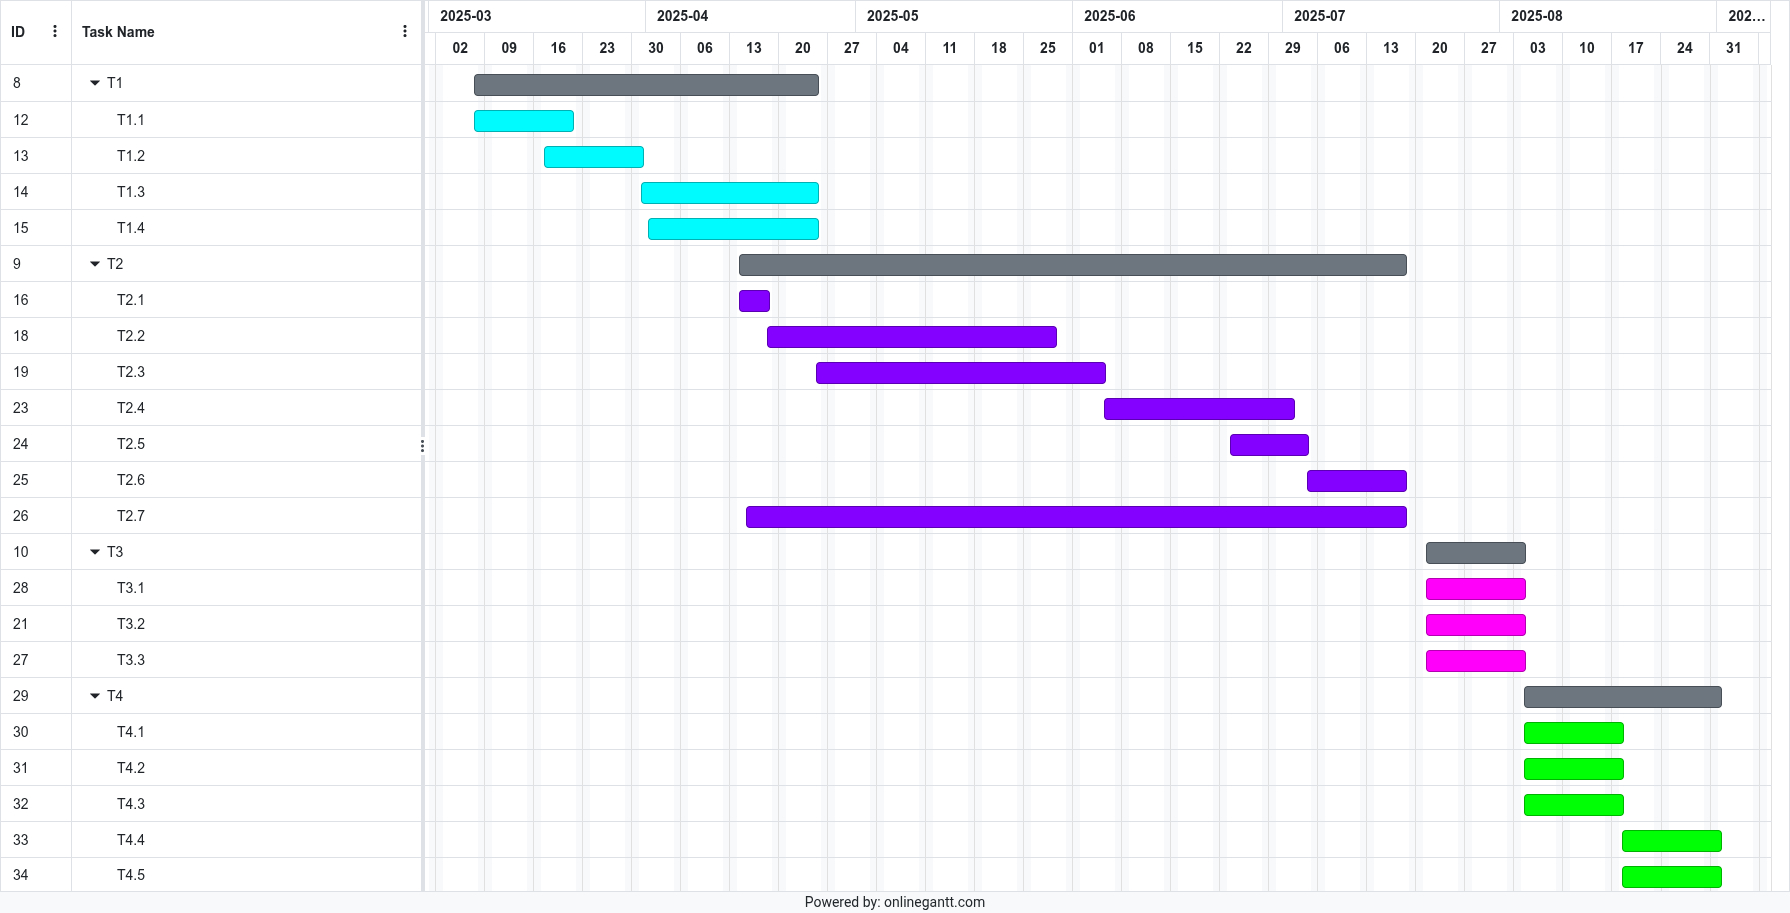
\includegraphics[width=\textwidth]{imagenes/cap2/diagrama_gantt.png}
      \caption{Diagrama de Gantt del proyecto realizado en Online Gantt\footnote{\url{https://www.onlinegantt.com/}}}
      \label{fig:diagrama-gantt}
\end{figure}

\section{Estimación de costes}

A continuación, se detallan los recursos necesarios para llevar a cabo el proyecto, incluyendo hardware, software y recursos humanos, junto con una estimación de los costes asociados.

\subsubsection{Hardware}

\begin{itemize}[noitemsep]
      \item Ordenador portátil LG Gram 14Z90Q-G.AA75B, este equipo se utilizará para el desarrollo general del trabajo: creación del código para las pruebas y creación de la memoria.

      \item Ordenador portátil Lenovo Legion 5, utilizado como plataforma principal para la ejecución de pruebas de rendimiento.

      \item Ordenador Apple Mac Mini M4, utilizado como plataforma de pruebas para la ejecución y validación de aplicaciones HPC en entornos macOS.
\end{itemize}

\subsection{Recursos humanos}

\begin{table}[!ht]
      \centering
      \begin{tabular}{|l|l|r|}
            \hline
            \textbf{Dispositivo}   & \textbf{Descripción}             & \textbf{Coste (€)} \\
            \hline
            LG Gram 14Z90Q-G.AA75B & Portátil principal de desarrollo & 1\,000             \\
            Lenovo Legion 5        & Portátil de pruebas              & 500                \\
            Apple Mac Mini M4      & Dispositivo de pruebas Apple     & 599                \\
            \hline
            \textbf{Total}         &                                  & \textbf{2\,099}    \\
            \hline
      \end{tabular}
      \caption{Costes estimados de hardware para el proyecto}
      \label{tab:costes-hardware}
\end{table}

En la tabla \ref{tab:recursos-humanos} se detalla el coste por hora, las horas estimadas y el coste total de los recursos humanos necesarios para llevar a cabo el proyecto.

\begin{table}[!ht]
      \centering
      \begin{tabular}{|l|l|r|r|r|}
            \hline
            \textbf{Recurso}        & \textbf{Puesto}  & \textbf{€/h} & \textbf{Horas} & \textbf{Total (€)} \\
            \hline
            Fernando Cuesta Bueno   & Desarrollador    & 15           & 260            & 3\,750             \\
            Juan José Escobar Pérez & Tutor/Supervisor & 25           & 50             & 1\,750             \\
            \hline
            \textbf{Total}          &                  &              &                & \textbf{5\,500}    \\
            \hline
      \end{tabular}
      \caption{Costes estimados de recursos humanos para el proyecto}
      \label{tab:recursos-humanos}
\end{table}

El coste por hora del desarrollador ha sido obtenido a partir del salario medio por hora indicado en la página web \cite{joobleIngenieroInformatico}. Esta página recoge datos de diversas fuentes para calcular el salario medio en España para un ingeniero informático, que es de $17,98$€/h. Dado que el proyecto se realiza en el ámbito académico y no profesional, se ha estimado un coste por hora de $15$€/h para el desarrollador. Por otro lado, el coste por hora del tutor se ha estimado en $25$€/h, considerando su experiencia y rol de supervisión en el proyecto.


\subsection{Coste total del proyecto}

En el supuesto de que el proyecto se realizara en un entorno profesional, habría que considerar una cuota empresarial de un $30\%$ sobre el coste mostrado en la tabla \ref{tab:recursos-humanos}.

El coste total del proyecto se calcula sumando los costes de hardware y de recursos humanos. En la tabla \ref{tab:coste-total} se detalla el coste total estimado.

\begin{table}[!ht]
      \centering
      \begin{tabular}{|l|r|}
            \hline
            \textbf{Concepto} & \textbf{Coste (€)} \\
            \hline
            Hardware          & 2\,099             \\
            Recursos humanos  & 5\,500             \\
            Cuota empresarial & 1\,650             \\
            \hline
            \textbf{Total}    & \textbf{9\,249}    \\
            \hline
      \end{tabular}
      \caption{Coste total estimado del proyecto}
      \label{tab:coste-total}
\end{table}
%
\chapter{Estado del arte}\label{cap:estado_del_arte}
[En el estado del arte se necesita hacer un estudio tanto sobre la tecnología que soporta el proyecto como sobre el problema que se aborda en él. Se puede estructurar por secciones y se aconseja utilizar referencias a los documentos e información que se describe aquí.

    Como norma general y más en proyectos con carácter investigador, se recomienda añadir un párrafo por cada documento/referencia que estudie del estado del arte, finalizando esta sección con un párrafo explicativo de la novedad/característica que propone, modifica o añade el proyecto sobre dicho estado del arte.]

\section{Sección}\label{sec:seccion}


\subsection{Sub-seccion}\label{sec:subsection}
%
\chapter{Propuesta principal}\label{cap:propuesta}

% [En esta sección se ha de introducir y explicar la propuesta principal del trabajo. Se puede y es recomendable dividir en secciones, incluso, este capítulo puede contemplar varios  capítulos a su vez.]

\section{Introducción de la propuesta}\label{sec:introduccion_propuesta}
En esta sección se presenta la propuesta general del trabajo, explicando la metodología seguida para evaluar el uso de contenedores en entornos HPC. Se justifica la elección de los experimentos en función de los objetivos del TFG y del estado del arte, y se define el alcance de los mismos, indicando qué se medirá y evaluará.

\section{Aplicación seleccionada: HPMoon}\label{sec:hpm_application}

\subsection{Origen y contexto}\label{subsec:hpm_origen}

HPMoon es un software desarrollado por el investigador Juan José Escobar Pérez en el marco de la tesis doctoral \textit{``Energy-Efficient Parallel and Distributed Multi-Objective Feature Selection on Heterogeneous Architectures''}. Su nombre proviene del proyecto \textit{High Performance Multi-Objective Optimization for Neuroengineering and Rehabilitation Technologies} (HPMoon), reflejando su enfoque en optimización de alto rendimiento y aplicaciones biomédicas.

El programa se concibe como una herramienta del proyecto \textit{e-hpMOBE} y está disponible públicamente en GitHub\footnote{\url{https://github.com/hpmoon/}}. Su desarrollo fue apoyado por proyectos de investigación nacionales financiados por el Ministerio de Ciencia, Innovación y Universidades (MICIU) y fondos FEDER, así como por una beca de NVIDIA.

Esta aplicación se utiliza como caso de estudio en este TFG debido a su relevante aportación científica y tecnológica en el ámbito de la computación de alto rendimiento (\acs{HPC}).

\subsection{Objetivo de HPMoon}\label{subsec:hpm_objetivo}
El objetivo principal de HPMoon es abordar la clasificación no supervisada de señales de Electroencefalograma (\acs{EEG}) en tareas de Interfaz Cerebro-Computadora (\acs{BCI}). Este es un problema de alta dimensionalidad y computacionalmente costoso debido a las características de las señales \acs{EEG} y al gran número de características que pueden contener. La aplicación combina la selección de características multiobjetivo (\acs{MOFS}) con algoritmos paralelos y energéticamente eficientes, buscando minimizar el tiempo de ejecución y el consumo de energía, cruciales en problemas de \textit{Machine Learning} y bioingeniería que requieren plataformas de alto rendimiento.

\subsection{Arquitectura y funcionamiento}\label{subsec:hpm_funcionamiento}

HPMoon implementa un procedimiento paralelo multinivel y energéticamente eficiente para la selección de características multiobjetivo (\acs{MOFS}). La versión más avanzada, conocida como ODGA, ha sido descrita como la ``más eficiente desarrollada hasta la fecha''. Su arquitectura combina técnicas de algoritmos evolutivos, paralelismo en múltiples niveles y optimización de recursos para abordar problemas complejos de selección de características.

El enfoque principal de HPMoon es de tipo wrapper, utilizando un Algoritmo Genético Multiobjetivo (MOGA), basado en una adaptación de NSGA-II, para seleccionar las características más relevantes. Cada individuo en la población representa una combinación posible de características y se evalúa mediante un procedimiento de fitness basado en el algoritmo K-means para clasificación no supervisada. La evaluación se realiza considerando dos funciones de coste: $f_1$, que minimiza la suma de distancias dentro de los clústeres (WCSS), y $f_2$, que maximiza la distancia entre centroides (BCSS). Ambas funciones se normalizan en el intervalo (0,1) para garantizar comparabilidad.

HPMoon explota hasta cuatro niveles de paralelismo en arquitecturas heterogéneas. A nivel de clúster, se distribuyen las tareas entre nodos utilizando MPI. Dentro de cada nodo, OpenMP gestiona la distribución de trabajo entre dispositivos CPU y GPU, mientras que a nivel de CPU se aprovechan múltiples hilos o unidades de cómputo (CUs). En la GPU, el paralelismo de datos se aplica al algoritmo K-means, acelerando el cálculo de distancias y la actualización de centroides.

El software está desarrollado principalmente en C++ e integra tecnologías HPC estándar: MPI para comunicación entre nodos, OpenMP para paralelismo en CPU y OpenCL para ejecutar los kernels de K-means en GPU. Además, incorpora esquemas master-worker con balanceo dinámico de carga, tanto entre CPU y GPU como entre nodos del clúster, optimizando la distribución de trabajo y minimizando desequilibrios, especialmente en versiones avanzadas como ODGA.

La configuración y ejecución de HPMoon se realiza desde la línea de comandos, permitiendo ajustar parámetros como el número de subpoblaciones, tamaño de la población, migraciones, generaciones, número de características y uso de CPU o GPU mediante un archivo XML. Esta flexibilidad facilita la adaptación del programa a distintos entornos de HPC y diferentes conjuntos de datos, maximizando eficiencia y reproducibilidad.

\subsection{Justificación de la elección para este TFG}\label{subsec:hpm_justificacion}

HPMoon se ha seleccionado como caso de estudio por varias razones que lo convierten en un candidato ideal para analizar aspectos como portabilidad, rendimiento y overhead de contenedores en entornos HPC. En primer lugar, su relevancia científica y tecnológica es clara: aborda un problema intensivo en cómputo, la clasificación de señales EEG de alta dimensionalidad, común en bioinformática e ingeniería biomédica. La complejidad de estas tareas permite generar métricas significativas de rendimiento en HPC.

Otro factor clave es su diseño para paralelización multinivel y arquitecturas heterogéneas. HPMoon explota múltiples niveles de paralelismo en CPUs multi-núcleo, GPUs y sistemas distribuidos en clústeres, lo que permite realizar análisis exhaustivos en distintas configuraciones. A esto se suma un énfasis en la eficiencia energética, optimizando tanto el consumo de energía como el tiempo de ejecución, un aspecto crítico en la computación de alto rendimiento moderna. Asimismo, incorpora estrategias de balanceo de carga dinámico entre CPU y GPU, lo que facilita manejar las diferencias de capacidad y consumo energético de dispositivos heterogéneos.

La disponibilidad y madurez del software también influyen en su elección. HPMoon es un proyecto robusto derivado de tesis doctoral y publicaciones científicas, con múltiples versiones evolutivas (SGA, PGA, OPGA, MDGA, MPGA, DGA, DGA-II, ODGA, GAAM) y documentación completa. Además, incluye modelos de energía-tiempo que permiten predecir el comportamiento de los algoritmos en sistemas monocomputador y distribuidos, proporcionando una base sólida para comparar resultados obtenidos en contenedores. Por último, la complejidad y los desafíos de optimización que presenta —como el balanceo de carga en entornos heterogéneos, irregularidades en accesos a memoria y la gestión de comunicación entre nodos y dispositivos— lo hacen ideal para evaluar el impacto de los contenedores en la eficiencia y optimización del código.

\subsection{Configuración y parámetros de compilación y ejecución}\label{subsec:hpm_configuracion}

La aplicación HPMoon requiere una fase previa de compilación y, posteriormente, una configuración en tiempo de ejecución a través de un fichero XML (con soporte parcial mediante parámetros de línea de comandos).

\subsubsection{Compilación}

La compilación de HPMoon se realiza a través de un \textit{Makefile}, que permite configurar los parámetros más importantes antes de generar el ejecutable. Entre estos parámetros destacan el número de características de la base de datos (\texttt{N\_FEATURES} o NF), que debe definirse entre 4 y el máximo disponible, y el compilador MPI a utilizar (\texttt{COMP} o COMPILER), que por defecto es \texttt{mpic++}.

Estos valores se procesan en tiempo de compilación, lo que permite evitar el uso de memoria dinámica innecesaria y maximizar el rendimiento del programa. Una vez completada la compilación, el ejecutable resultante, llamado \texttt{hpmoon}, se encuentra disponible en el directorio \texttt{bin}, listo para su ejecución en los distintos entornos de HPC.

\subsubsection{Configuración en tiempo de ejecución}

La configuración en tiempo de ejecución se realiza principalmente mediante un fichero XML, que permite ajustar tanto los parámetros de los algoritmos evolutivos como la gestión de recursos computacionales. Los parámetros más relevantes son:

\begin{itemize}
    \item \textbf{NSubpopulations}: número total de subpoblaciones (modelo de islas).
    \item \textbf{SubpopulationSize}: tamaño de cada subpoblación (número de individuos).
    \item \textbf{NGlobalMigrations}: número de migraciones entre subpoblaciones en diferentes nodos.
    \item \textbf{NGenerations}: número de generaciones a simular.
    \item \textbf{MaxFeatures}: número máximo de características permitidas.
    \item \textbf{DataFileName}: fichero de salida con la aptitud de los individuos del primer frente de Pareto.
    \item \textbf{PlotFileName}: fichero con el código de gnuplot para visualización.
    \item \textbf{ImageFileName}: fichero de salida con la gráfica generada.
    \item \textbf{TournamentSize}: número de individuos en el torneo de selección.
    \item \textbf{NInstances}: número de instancias (filas) de la base de datos a utilizar.
    \item \textbf{FileName}: nombre del fichero de la base de datos de entrada.
    \item \textbf{Normalize}: indica si la base de datos debe ser normalizada.
    \item \textbf{NDevices}: número de dispositivos OpenCL empleados en el nodo.
    \item \textbf{Names}: lista de nombres de dispositivos OpenCL, separados por comas.
    \item \textbf{ComputeUnits}: unidades de cómputo por dispositivo OpenCL, en el mismo orden que \texttt{Names}.
    \item \textbf{WiLocal}: número de \textit{work-items} por unidad de cómputo, alineado con los dispositivos.
    \item \textbf{CpuThreads}: número de hilos de CPU para la evaluación de aptitud. Si es 1 y \texttt{NDevices=0}, la ejecución es secuencial.
    \item \textbf{KernelsFileName}: fichero con los kernels de OpenCL.
\end{itemize}

Muchos de estos parámetros pueden especificarse también mediante opciones en la línea de comandos al ejecutar \texttt{hpmoon}, aunque no todos están disponibles de esta forma. Esta circunstancia se refleja en la columna \texttt{CMD OPTION} de la Tabla~\ref{tab:hpmoon_parametros}, donde un guion (\texttt{-}) indica ausencia de soporte por línea de comandos.

\begin{table}[htbp]
    \centering
    \footnotesize
    \setlength{\tabcolsep}{3pt}
    \begin{tabular}{|p{3cm}|p{6cm}|p{2.2cm}|}
        \hline
        \textbf{PARÁMETRO}  & \textbf{RANGO}                                                          & \textbf{CMD OPTION} \\ \hline
        N\_FEATURES         & $4 \leq \mathrm{NF} \leq$ Número de características de la base de datos & -                   \\ \hline
        NSubpopulations     & $1 \leq \mathrm{NP}$                                                    & -ns                 \\ \hline
        SubpopulationSize   & $4 \leq \mathrm{PS}$                                                    & -ss                 \\ \hline
        NGlobalMigrations   & $1 \leq \mathrm{NM}$                                                    & -ngm                \\ \hline
        NGenerations        & $0 \leq \mathrm{NG}$                                                    & -g                  \\ \hline
        MaxFeatures         & $1 \leq \mathrm{MaxF}$                                                  & -maxf               \\ \hline
        DataFileName        & Nombre de fichero válido                                                & -plotdata           \\ \hline
        PlotFileName        & Nombre de fichero válido                                                & -plotsrc            \\ \hline
        ImageFileName       & Nombre de fichero válido                                                & -plotimg            \\ \hline
        TournamentSize      & $2 \leq \mathrm{TS}$                                                    & -ts                 \\ \hline
        NInstances          & $4 \leq \mathrm{NI} \leq$ Número de instancias de la base de datos      & -trni               \\ \hline
        FileName            & Base de datos de entrenamiento existente                                & -trdb               \\ \hline
        Normalize           & 1 ó 0                                                                   & -trnorm             \\ \hline
        NDevices            & $0 \leq \mathrm{ND}$                                                    & -                   \\ \hline
        Names               & Nombre de dispositivo existente                                         & -                   \\ \hline
        ComputeUnits        & $1 \leq \mathrm{CU}$                                                    & -                   \\ \hline
        WiLocal             & $1 \leq \mathrm{WL} \leq$ Máx. work-items locales del dispositivo       & -                   \\ \hline
        CpuThreads          & $0 \leq \mathrm{CT}$                                                    & -                   \\ \hline
        KernelsFileName     & Fichero de kernels existente                                            & -ke                 \\ \hline
        Display usage       & -                                                                       & -h                  \\ \hline
        List OpenCL devices & -                                                                       & -l                  \\ \hline
    \end{tabular}
    \caption{Rango de valores de los parámetros de entrada y su uso desde la línea de argumentos (si está disponible).}
    \label{tab:hpmoon_parametros}
\end{table}

\subsection{Selección de parámetros de estudio}

La elección de los parámetros para este estudio se centró en mantener la mayoría de los valores por defecto y analizar únicamente la relación entre el número de subpoblaciones y el número de hilos. Esta decisión se basa en la arquitectura de paralelismo multinivel de HPMoon y su impacto directo en la distribución de la carga de trabajo y el rendimiento. A continuación, se detalla la justificación de esta selección.

\subsubsection{Paralelismo multinivel del programa}

HPMoon está diseñado como un algoritmo evolutivo que utiliza subpoblaciones y explota paralelismo en múltiples niveles. A nivel de clúster, MPI (Message Passing Interface) distribuye las subpoblaciones entre los distintos nodos. Dentro de cada nodo, OpenMP se encarga de repartir dinámicamente el trabajo entre los dispositivos disponibles, incluyendo CPU y GPU. La evaluación de la aptitud de los individuos combina OpenMP en la CPU y OpenCL en la GPU, ofreciendo hasta tres niveles de paralelismo en la CPU y cuatro en la GPU. Esta arquitectura multinivel es la que determina la elección de parámetros clave para el estudio.

\subsubsection{Número de subpoblaciones}

El parámetro \texttt{NSubpopulations} representa el número total de subpoblaciones y es fundamental para el modelo de islas del algoritmo. Incrementar este número puede mejorar la calidad de los resultados más que simplemente aumentar la población de individuos, según se indica en estudios previos \cite{escobar2020energy}. Además, define cómo se distribuye el trabajo a nivel de MPI entre los nodos y cómo estas unidades se gestionan posteriormente con OpenMP dentro de cada nodo.

\subsubsection{Número de hilos en CPU y GPU}

El programa hace un uso intensivo de hilos para la evaluación de la aptitud. En la CPU, el parámetro \texttt{CpuThreads} indica cuántos hilos se utilizan, y se recomienda que coincida con el número de núcleos lógicos para obtener un buen rendimiento. En la GPU, parámetros como \texttt{NDevices} (número de dispositivos OpenCL), \texttt{ComputeUnits} (unidades de cómputo) y \texttt{WiLocal} (hilos por unidad de cómputo) son esenciales. Ajustar \texttt{WiLocal} como múltiplo de 32 o 64 mejora la eficiencia de OpenCL, y la combinación óptima de estos valores depende del problema y del dispositivo. Estos parámetros controlan la paralelización de la función de evaluación en la GPU y la distribución dinámica de individuos mediante OpenMP \cite{escobar2020energy}.

\subsubsection{Número de nodos}

HPMoon está preparado para ejecutarse en sistemas distribuidos. En la versión DGA (Distributed Genetic Algorithm), las subpoblaciones se reparten entre nodos usando MPI, agregando un cuarto nivel de paralelismo. El nodo maestro (MPI 0) gestiona esta distribución de manera dinámica. La escalabilidad y el rendimiento dependen directamente del número de nodos: aumentar su cantidad puede reducir significativamente el tiempo de ejecución y el consumo energético, alcanzando speedups de hasta 83 veces y reduciendo el consumo de energía a menos del 5\% en el mejor de los casos \cite{escobar2020energy, Escobar2019}. Además, la heterogeneidad de los nodos y su configuración de CPU/GPU influyen en la eficiencia de la distribución de carga.

\subsubsection{Razones para mantener otros parámetros por defecto}

Se decidió no modificar el resto de los parámetros por varias razones. Primero, la prioridad del estudio es entender cómo el paralelismo y la asignación de recursos influyen en el rendimiento, por lo que se enfocó en \texttt{NSubpopulations} y en los hilos de CPU/GPU. Segundo, algunos parámetros como \texttt{N\_FEATURES} se fijan en tiempo de compilación, lo que dificulta su ajuste en pruebas de rendimiento. Tercero, la función de evaluación (K-means) consume más del 99\% del tiempo de ejecución para poblaciones moderadas, por lo que optimizar su paralelización es crítico \cite{escobar2020energy}. Otros parámetros secundarios relacionados con el algoritmo evolutivo o la gestión de datos no afectan de manera tan directa al comportamiento fundamental del paralelismo. Por último, estudiar bases de datos muy grandes podría provocar problemas de memoria en la GPU, por lo que es más prudente analizar estos factores una vez comprendido el paralelismo básico.

En resumen, al concentrarse en el número de subpoblaciones, el número de hebras y el número de nodos, se aborda directamente la capacidad del programa para aprovechar arquitecturas paralelas y la distribución de la carga de trabajo en todos los niveles, sentando las bases para análisis más detallados posteriormente \cite{escobar2020energy}.

\subsection{Diseño de los experimentos}\label{subsec:diseno_experimentos_detallado}

Los experimentos se estructuran en varias fases con el fin de determinar los parámetros óptimos y evaluar la escalabilidad y portabilidad de HPMoon en distintos entornos y plataformas.

\subsubsection{Determinación del número óptimo de subpoblaciones}\label{subsubsec:determinacion_subpoblaciones}

Se realizarán ejecuciones exploratorias con distintas configuraciones de subpoblaciones y hebras, para definir el parámetro de \texttt{NSubpopulations}, así como el de \texttt{CpuThreads}, a usar en los tests posteriores:

\begin{itemize}
    \item Se lanzarán ejecuciones con 1, 2, 4, 8 y 16 subpoblaciones.
    \item Para cada configuración de subpoblaciones, se evaluará con 1, 2, 4, 8 y 16 hebras por subpoblación.
\end{itemize}

\subsubsection{Estudio del rendimiento al requerir más hebras de las disponibles}

Uno de los experimentos planteados consiste en evaluar el rendimiento de la aplicación realizando un barrido completo de todas las combinaciones posibles de número de nodos y de hebras por nodo. Dado que el dispositivo en el que se realizarán los tests cuenta con un máximo de 16 hebras, resulta especialmente interesante analizar cómo se comporta la aplicación cuando se solicita un número de hebras superior al disponible. Este estudio permitirá determinar si es necesario imponer un límite en el número de hebras para los tests posteriores.

En las ejecuciones multinodo, cada nodo se configurará con un número de hebras tal que el total de hebras activas sea igual al producto del número de nodos por el número de hebras por nodo. Para explorar el comportamiento de la aplicación en escenarios límite, se plantean dos variantes de prueba: en la primera, si el número total de hebras requerido supera el máximo del dispositivo (16), el test no se ejecuta; en la segunda, se permiten ejecuciones aunque la cantidad de hebras solicitadas exceda el límite del hardware. Con esto se pretende identificar si el rendimiento se degrada o si el sistema puede manejar de manera eficiente solicitudes superiores a la capacidad real, estableciendo así las condiciones óptimas para los experimentos posteriores.

\subsubsection{Estudio del rendimiento al utilizar la misma GPU en todos los nodos}

En un escenario multinodo local, donde los nodos corresponden a procesos distribuidos dentro de un mismo dispositivo, resulta importante analizar cómo el uso de la GPU afecta al rendimiento de HPMoon. El dispositivo disponible cuenta con una única tarjeta gráfica, por lo que se consideran dos configuraciones posibles.

En la primera, todos los nodos comparten la misma GPU, lo que permite evaluar el impacto de la contención del recurso gráfico cuando varios procesos intentan ejecutar cálculos en paralelo sobre la misma tarjeta. En la segunda configuración, la GPU se asigna únicamente a un nodo, mientras que el resto de nodos realiza los cálculos exclusivamente con la CPU. Este enfoque permite medir si centralizar el uso de la GPU en un solo nodo mejora la eficiencia global frente al acceso compartido.

El objetivo de este estudio es identificar cuál de estas estrategias ofrece un mejor rendimiento en configuraciones multinodo locales. Para ello se analizará la eficiencia en términos de tiempo total de cálculo y utilización de recursos, se evaluará la escalabilidad de la aplicación al incrementar el número de nodos y se extraerán recomendaciones sobre la asignación de la GPU en futuras pruebas multinodo. De esta manera, se podrá determinar si resulta más eficiente que todos los nodos compartan la GPU o si es preferible que solo uno de ellos la utilice, teniendo en cuenta tanto el rendimiento como la complejidad de gestión de los recursos.

\subsubsection{Experimentos de escalabilidad}

Una vez definido el número óptimo de subpoblaciones, el rango válido de hebras y la estrategia de uso de la GPU en entornos multinodo, se realizarán los siguientes experimentos:

\begin{itemize}
    \item \textbf{Escalabilidad mononodo:} con un único nodo fijo, se escala el número de hebras.
    \item \textbf{Escalabilidad multinodo:} con una única hebra por nodo, se escala el número de nodos.
    \item \textbf{Barrido de hebras:} se ejecutan todas las combinaciones posibles de número de nodos y hebras por nodo.
\end{itemize}

\subsubsection{Plataformas y entornos de ejecución}

Los experimentos se realizarán en distintas plataformas y entornos, tanto con uso único de CPU como la combinación con uso de GPU (salvo en el caso de Mac, donde el uso de GPU en contenedores es objeto de estudio):

\begin{itemize}
    \item Ubuntu 24.04: ejecución nativa, y en contenedores Docker y Podman.
    \item Windows 11 Home: ejecución en contenedores Docker y Podman.
    \item MacOS Sequoia 15.5: ejecución en contenedores Docker y Podman.
\end{itemize}

Esta estructura permitirá evaluar la escalabilidad, portabilidad y rendimiento de HPMoon en entornos contenerizados y nativos, así como en arquitecturas heterogéneas con CPU y GPU.

\section{Herramientas y scripts utilizados}\label{sec:herramientas_scripts}

La carpeta de scripts está organizada en subcarpetas y archivos que se pueden agrupar según su función principal en cuatro bloques:

\subsection{Compilación y preparación}
Incluye scripts como \textit{build\_hpmoon.sh} y \textit{clean\_system.sh} dentro de la carpeta \texttt{utils}. Su objetivo es automatizar la compilación del software HPMoon y preparar el entorno, asegurando que el binario esté actualizado y que el sistema esté limpio antes de cada experimento.

\subsection{Pruebas de escalabilidad}

En esta categoría se agrupan los scripts que permiten evaluar cómo HPMoon se comporta frente a diferentes configuraciones de hardware y parámetros del algoritmo, así como explorar de manera sistemática todas las combinaciones posibles de nodos y hebras. Los scripts se organizan en subcarpetas como \textit{single-node}, \textit{multi-node}, \textit{experiments} y \textit{thread-sweep}, e incluyen ejemplos como \textit{run\_ubuntu\_native.sh}, \textit{run\_ubuntu\_native\_limit.sh} o \textit{run\_ubuntu\_container.sh}.

El objetivo de estos scripts es doble: por un lado, analizar la escalabilidad y el rendimiento de la aplicación en entornos nativos y contenerizados; por otro, generar un panorama completo de cómo diferentes parámetros afectan la ejecución, permitiendo realizar barridos sistemáticos que produzcan matrices completas de resultados.

De manera más concreta, los scripts permiten:

\begin{itemize}
    \item Variar parámetros críticos como el número de nodos, el número de hebras por nodo y el número de subpoblaciones, observando cómo influyen en el tiempo de ejecución y en la eficiencia general.
    \item Comparar el comportamiento de la aplicación en entornos nativos frente a entornos contenerizados, evaluando el overhead introducido por la virtualización.
    \item Realizar barridos exhaustivos de parámetros, registrando resultados para todas las combinaciones posibles de nodos y hebras, de manera que se puedan identificar configuraciones óptimas y detectar posibles cuellos de botella.
\end{itemize}

Gracias a esta organización y automatización, se puede estudiar de forma sistemática la eficiencia, la escalabilidad y el comportamiento de HPMoon en distintas plataformas, garantizando resultados reproducibles y comparables.

\subsection{Automatización total y orquestación}
Incluye scripts de alto nivel como \textit{run\_ubuntu\_all.sh} o \textit{run\_windows\_all.sh}, que coordinan compilación, ejecución y recolección de resultados de forma secuencial.

\subsection{Valor añadido e innovación}

Los scripts desarrollados aportan un valor significativo al estudio al combinar automatización, flexibilidad y reproducibilidad. Permiten ejecutar campañas de pruebas complejas con un solo comando, minimizando errores humanos y optimizando el tiempo de ejecución. Al mismo tiempo, facilitan la modificación rápida de parámetros clave sin intervención manual, lo que permite explorar distintas configuraciones de nodos, hebras y subpoblaciones de manera eficiente. Su estructura también posibilita comparar de forma sistemática el rendimiento entre ejecuciones nativas y contenerizadas, así como entre distintas plataformas, asegurando resultados homogéneos y fácilmente interpretables. Además, estos scripts soportan escenarios multinodo y multiplataforma, validando la escalabilidad y la portabilidad de HPMoon en distintos entornos de HPC. Finalmente, la gestión organizada de logs y resultados garantiza que los experimentos sean completamente reproducibles y auditables, alineándose con las buenas prácticas científicas.

\section{Repositorio del proyecto}\label{sec:repositorio}

Todo el trabajo desarrollado en este TFG, incluyendo scripts, configuraciones, documentación y resultados de los experimentos, está recogido y disponible públicamente en un repositorio de GitHub\footnote{\url{https://github.com/FerniCuesta/DockEEG}}.

%
\chapter{Experimentación}\label{cap:experimentacion}

\section{Experimentos preliminares}

En esta primera fase de experimentacion se realizarán pruebas para determinar los parámetros óptimos de ejecución y estudiar el rendimiento de la aplicación en distintos entornos y plataformas.

\subsection{Determinación del número óptimo de subpoblaciones y hebras}

Como se ha comentado en la sección \ref{subsubsec:determinacion_subpoblaciones}, se realizarán ejecuciones exploratorias con distintas configuraciones de subpoblaciones y hebras, para definir el parámetro de \texttt{NSubpopulations} a usar en los tests posteriores.

En la figura \ref{fig:exploratory_subpopulations} se muestran los datos de estas ejecuciones exploratorias. Se observa que para cualquier número de subpoblaciones, el comportamiento es similar. En la tabla \ref{tab:exploratory_subpopulations_times} se presentan los tiempos de ejecución en segundos para cada combinación de hebras y subpoblaciones, al incrementar el número de subpoblaciones también aumenta significativamente el tiempo de ejecución, especialmente cuando se utilizan pocas hebras.

\begin{figure}[ht]
    \centering
    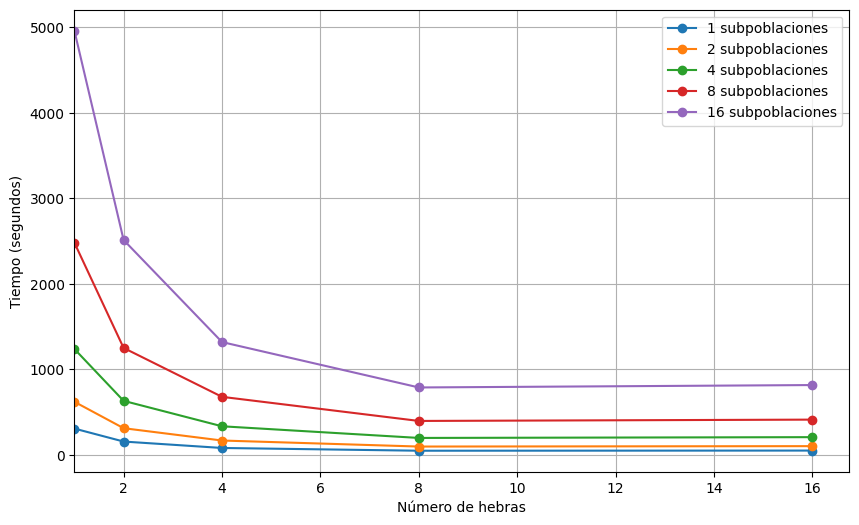
\includegraphics[width=0.8\textwidth]{imagenes/cap5/exploratory_subpopulations.png}
    \caption{Gráficas de ejecución de las pruebas variando el número de subpoblaciones y hebras.}
    \label{fig:exploratory_subpopulations}
\end{figure}

\begin{table}[ht]
    \centering
    \begin{tabular}{|c|ccccc|}
        \hline
        \multirow{2}{*}{\textbf{Hebras}} & \multicolumn{5}{c|}{\textbf{Subpoblaciones}}                                                      \\ \cline{2-6}
                                         & \textbf{1}                                   & \textbf{2} & \textbf{4} & \textbf{8} & \textbf{16} \\ \hline
        1                                & 309.43                                       & 622.63     & 1239.73    & 2481.89    & 4960.00     \\ \hline
        2                                & 157.79                                       & 313.86     & 633.66     & 1252.12    & 2513.72     \\ \hline
        4                                & 82.73                                        & 169.76     & 336.25     & 680.46     & 1320.66     \\ \hline
        8                                & 50.58                                        & 99.37      & 200.01     & 398.66     & 790.04      \\ \hline
        16                               & 52.32                                        & 104.06     & 209.17     & 414.11     & 818.17      \\ \hline
    \end{tabular}
    \caption{Tiempos de ejecución en segundos de las pruebas variando el número de subpoblaciones y hebras.}
    \label{tab:exploratory_subpopulations_times}
\end{table}

En la tabla \ref{tab:exploratory_populations_delta} se presentan los porcentajes de reducción del tiempo de ejecución respecto a la configuración base. En cada columna, la ejecución con una sola hebra y una sola subpoblación se toma como referencia (0\% de variación). Estos resultados permiten cuantificar de manera objetiva el beneficio relativo derivado del incremento del paralelismo y de la subdivisión de la población, proporcionando una base empírica para identificar configuraciones óptimas de ejecución.

\begin{table}[ht]
    \centering
    \begin{tabular}{|c|ccccc|}
        \hline
        \multirow{2}{*}{\textbf{Hebras}} & \multicolumn{5}{c|}{\textbf{Subpoblaciones}}                                                      \\ \cline{2-6}
                                         & \textbf{1}                                   & \textbf{2} & \textbf{4} & \textbf{8} & \textbf{16} \\ \hline
        1                                & 0.00                                         & 0.00       & 0.00       & 0.00       & 0.00        \\ \hline
        2                                & 49.01                                        & 49.59      & 48.89      & 49.55      & 49.32       \\ \hline
        4                                & 73.26                                        & 72.74      & 72.88      & 72.58      & 73.37       \\ \hline
        8                                & 83.65                                        & 84.04      & 83.87      & 83.94      & 84.07       \\ \hline
        16                               & 83.09                                        & 83.29      & 83.13      & 83.31      & 83.50       \\ \hline
    \end{tabular}
    \caption{Porcentaje de variación del tiempo de ejecución respecto a la configuración base para distintas combinaciones de hebras y subpoblaciones}
    \label{tab:exploratory_populations_delta}
\end{table}

Del análisis de esta tabla pueden extraerse varias conclusiones de interés para la definición de los parámetros en los experimentos posteriores. En primer lugar, se observa que, para un número fijo de hebras, la variación en el tiempo es prácticamente inexistente al modificar el número de subpoblaciones, lo que indica que el comportamiento es proporcional con independencia de este parámetro. En segundo lugar, el mayor beneficio en términos de reducción del tiempo de ejecución se obtiene al incrementar el número de hebras de 1 a 8, alcanzando valores en torno al 83--84\%. Sin embargo, al pasar de 8 a 16 hebras, los tiempos de ejecución se incrementan en todos los casos, lo que revela que se ha sobrepasado el punto de paralelismo óptimo para la arquitectura hardware utilizada. Este resultado sugiere que, en el entorno experimental considerado, el uso de más de 8 hebras no proporciona mejoras de rendimiento adicionales e, incluso, puede resultar contraproducente debido a la sobrecarga y la contención de recursos.

No obstante, se ha decidido mantener configuraciones con 16 hebras en los experimentos posteriores con el fin de analizar el comportamiento bajo condiciones de sobrecarga, dado que el objetivo del estudio trasciende la mera optimización de un caso específico y busca evaluar la escalabilidad y el rendimiento en un rango amplio de escenarios. En cuanto al número de subpoblaciones, se constata que con 16 subpoblaciones los tiempos de ejecución pueden alcanzar hasta 1 hora y 20 minutos en configuraciones con una única hebra, lo que resulta excesivo para los objetivos de este trabajo. Por el contrario, con 8 subpoblaciones se obtienen tiempos de ejecución más razonables, se alcanza un equilibrio adecuado entre eficiencia y aprovechamiento de recursos, y se garantiza una buena escalabilidad.

En consecuencia, se justifica la decisión metodológica de fijar el número de subpoblaciones en 8 para los experimentos posteriores, al representar un compromiso óptimo entre eficiencia, utilización de recursos y escalabilidad en el entorno analizado.

\subsection{Estudio del rendimiento al requerir más hebras de las disponibles}

En esta sección se presentan los resultados de las ejecuciones exploratorias realizadas para analizar el rendimiento de la aplicación al variar el número de procesos y hebras, incluyendo configuraciones que superan el límite físico de hebras de la CPU (16 hebras). El objetivo es comprender cómo afecta esta variación al tiempo de ejecución y al uso efectivo de la CPU, proporcionando una base para la selección de parámetros en estudios posteriores.

En la figura \ref{fig:exploratory_threads_limit_time} se muestra la evolución del tiempo de ejecución en función del número de hebras asignadas por proceso, para configuraciones que van desde 1 hasta 16 procesos, pero limitando el número máximo de hebras a 16.

\begin{figure}[ht]
    \centering
    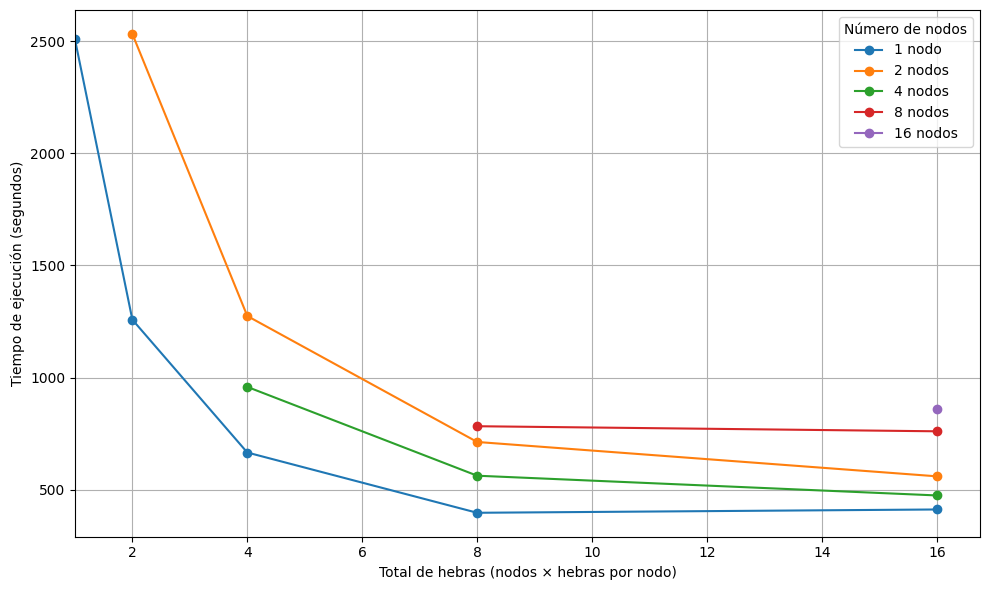
\includegraphics[width=0.8\textwidth]{imagenes/cap5/exploratory_threads_limit_time.png}
    \caption{Gráfica de tiempo de ejecución en función del número de hebras por proceso, con límite de 16 hebras.}
    \label{fig:exploratory_threads_limit_time}
\end{figure}

La figura \ref{fig:exploratory_threads_limit_cpu} muestra el porcentaje de uso total de CPU (donde 100\% equivale al uso completo de una hebra) para las distintas configuraciones de hebras por proceso analizadas.

\begin{figure}[ht]
    \centering
    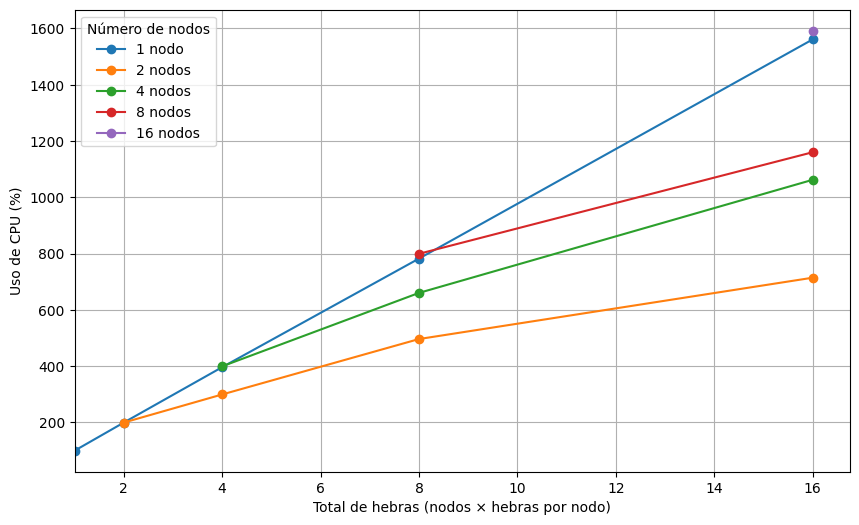
\includegraphics[width=0.8\textwidth]{imagenes/cap5/exploratory_threads_limit_cpu.png}
    \caption{Gráfica de uso de CPU en función del número de hebras por proceso, con límite de 16 hebras.}
    \label{fig:exploratory_threads_limit_cpu}
\end{figure}

Por otro lado, en la figura \ref{fig:exploratory_threads_no-limit_time} se presentan los resultados de las ejecuciones exploratorias sin límite en el número de hebras, permitiendo así evaluar el comportamiento del sistema al requerir más hebras de las disponibles.

\begin{figure}[ht]
    \centering
    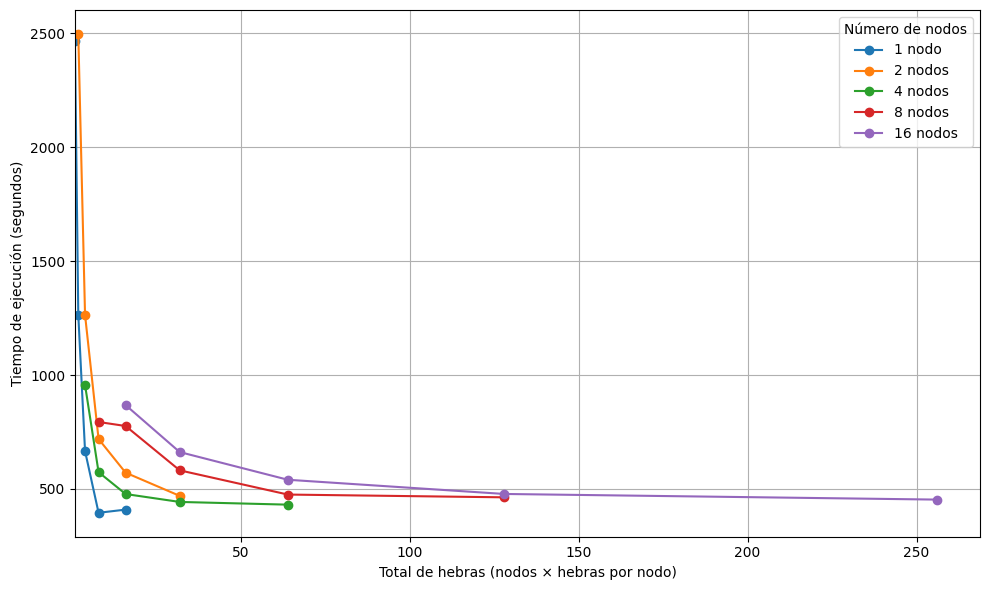
\includegraphics[width=0.8\textwidth]{imagenes/cap5/exploratory_threads_no-limit_time.png}
    \caption{Gráfica de tiempo de ejecución en función del número de hebras por proceso, sin límite en el número de hebras.}
    \label{fig:exploratory_threads_no-limit_time}
\end{figure}

La figura \ref{fig:exploratory_threads_no-limit_cpu} muestra el porcentaje de uso total de CPU para las distintas configuraciones de hebras por proceso sin límite, permitiendo observar cómo varía el aprovechamiento de los recursos en función del número total de hebras asignadas.

\begin{figure}[ht]
    \centering
    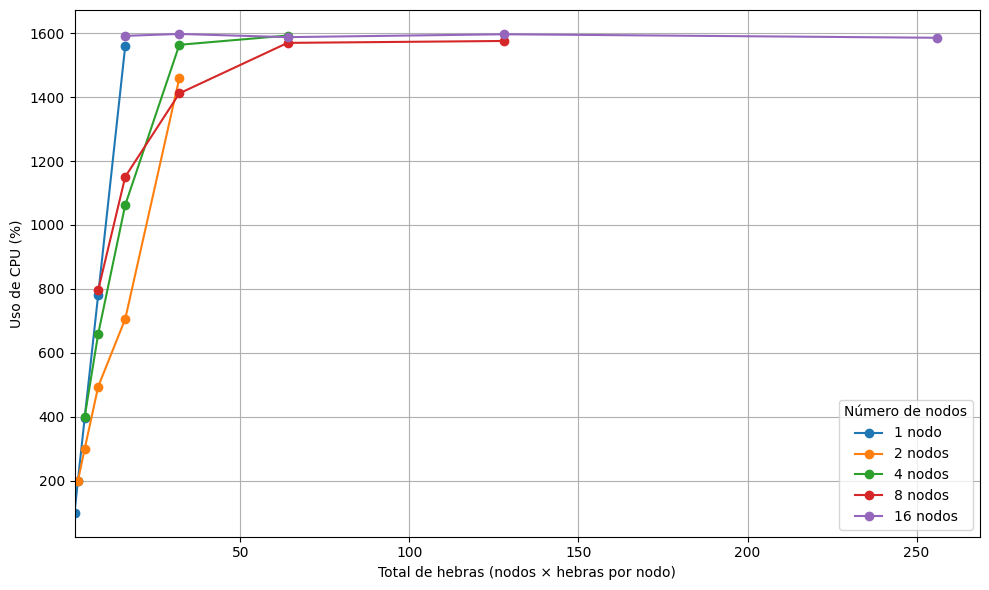
\includegraphics[width=0.8\textwidth]{imagenes/cap5/exploratory_threads_no-limit_cpu.png}
    \caption{Gráfica de uso de CPU en función del número de hebras por proceso, sin límite en el número de hebras.}
    \label{fig:exploratory_threads_no-limit_cpu}
\end{figure}

Las conclusiones que se pueden extraer de estas gráficas se pueden ver de manera más clara en la tabla \ref{tab:summary_nodes_threads_cpu}, donde se resumen los tiempos de ejecución y el uso de CPU para todas las combinaciones de procesos y hebras analizadas, tanto con límite como sin límite en el número de hebras.

\begin{table}[ht]
    \centering
    \small
    \setlength{\tabcolsep}{4pt}
    \renewcommand{\arraystretch}{1.1}
    \begin{tabular}{|c|c|c|c|c|}
        \hline
        \textbf{Procesos} & \textbf{Hebras}      & \textbf{Hebras}  & \textbf{Tiempo} & \textbf{Uso de}   \\
                          & \textbf{por proceso} & \textbf{totales} & \textbf{(s)}    & \textbf{CPU (\%)} \\
        \hline
        1                 & 8                    & 8                & 395.63          & 782               \\
        1                 & 16                   & 16               & 409.51          & 1561              \\
        4                 & 16                   & 64               & 431.30          & 1593              \\
        4                 & 8                    & 32               & 443.23          & 1564              \\
        16                & 16                   & 256              & 453.48          & 1586              \\
        8                 & 16                   & 128              & 463.45          & 1576              \\
        2                 & 16                   & 32               & 469.88          & 1460              \\
        8                 & 8                    & 64               & 475.59          & 1570              \\
        4                 & 4                    & 16               & 477.90          & 1063              \\
        16                & 8                    & 128              & 478.23          & 1597              \\
        16                & 4                    & 64               & 540.54          & 1588              \\
        2                 & 8                    & 16               & 571.65          & 706               \\
        4                 & 2                    & 8                & 573.94          & 659               \\
        8                 & 4                    & 32               & 581.91          & 1412              \\
        16                & 2                    & 32               & 662.10          & 1598              \\
        1                 & 4                    & 4                & 666.51          & 396               \\
        2                 & 4                    & 8                & 719.43          & 494               \\
        8                 & 2                    & 16               & 776.44          & 1151              \\
        8                 & 1                    & 8                & 794.09          & 796               \\
        16                & 1                    & 16               & 868.28          & 1592              \\
        4                 & 1                    & 4                & 956.38          & 399               \\
        2                 & 2                    & 4                & 1263.74         & 299               \\
        1                 & 2                    & 2                & 1264.94         & 199               \\
        1                 & 1                    & 1                & 2467.76         & 99                \\
        2                 & 1                    & 2                & 2497.06         & 199               \\
        \hline
    \end{tabular}
    \caption{Resumen de configuraciones de procesos, hebras y uso de CPU}
    \label{tab:summary_nodes_threads_cpu}
\end{table}

Los resultados muestran que el mejor rendimiento se alcanza empleando un menor número de procesos con un mayor número de hebras por proceso, siendo la configuración óptima la de un único proceso y ocho hebras. Aunque el límite físico de hebras de la CPU es de 16, se observa que, entre los diez mejores resultados, solo tres respetan este límite. En los demás casos, incrementar el número de hebras más allá de la capacidad física sigue proporcionando mejoras en el rendimiento, un comportamiento que, aunque inicialmente contraintuitivo, puede explicarse analizando el uso efectivo de la CPU.

El porcentaje de utilización de la CPU refleja el grado de aprovechamiento de las hebras disponibles: por ejemplo, con una hebra se alcanza un uso máximo de 100\%, con dos hebras el 200\%, y así sucesivamente hasta un máximo teórico de 1600\% (16 hebras $\times$ 100\%). En configuraciones de un único proceso, aumentar el número de hebras se traduce en un incremento proporcional del uso de CPU, lo que explica las mejoras de rendimiento observadas.

En contraste, cuando el número total de hebras se distribuye entre varios procesos, incluso si no se supera el límite físico de la CPU, el rendimiento no mejora de la misma manera. Esto se debe a la sobrecarga inherente a la gestión de múltiples procesos, que puede contrarrestar los beneficios de disponer de más hebras, haciendo que el uso efectivo de la CPU no alcance los valores esperados y resultando en un rendimiento inferior respecto a configuraciones monoproceso equivalentes. Por tanto, para configuraciones multiproceso es necesario incrementar el número de hebras más allá de la capacidad física de cada CPU para acercarse al uso máximo teórico, lo que explica por qué los mejores resultados se obtienen bajo estas condiciones.

\subsection{Estudio del rendimiento al utilizar la misma GPU en distintos procesos}

En esta sección se presentan los resultados de las ejecuciones exploratorias realizadas para analizar el rendimiento de la aplicación al variar el número de procesos y hebras, considerando dos enfoques distintos respecto al uso de la GPU: uno en el que se limita su uso a un único proceso y otro en el que se permite su uso en todos los procesos. El objetivo es comprender cómo afecta esta variación al tiempo de ejecución y al uso efectivo de la CPU, proporcionando una base para la selección de parámetros en estudios posteriores.

En la figura \ref{fig:exploratory_gpu_limit_time} se muestra la evolución del tiempo de ejecución en función del número de hebras asignadas por proceso, para configuraciones que van desde 1 hasta 16 procesos, limitando el uso de la GPU a un único proceso.

\begin{figure}[ht]
    \centering
    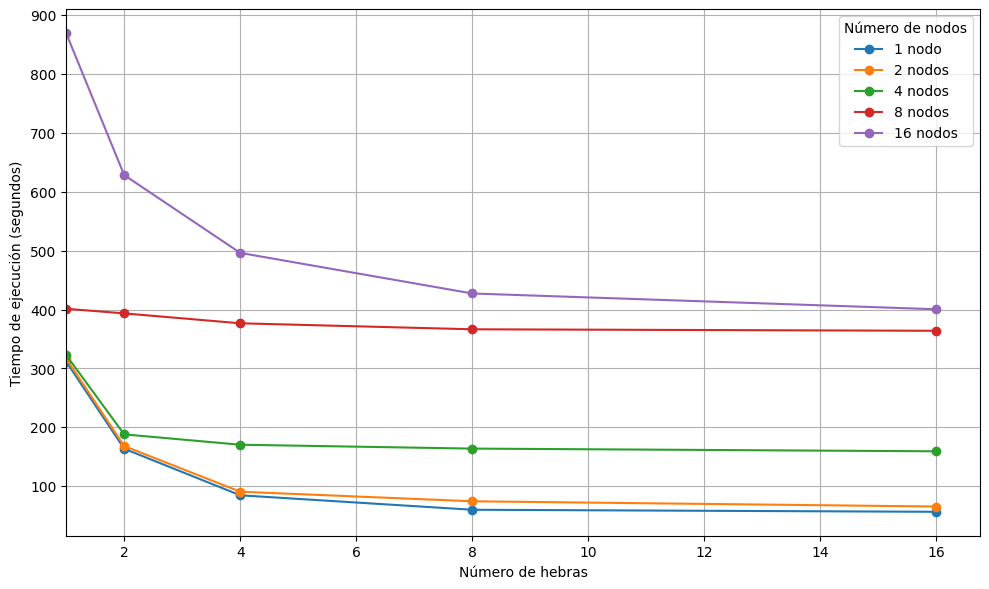
\includegraphics[width=0.8\textwidth]{imagenes/cap5/exploratory_gpu_limit_time.png}
    \caption{Gráfica de tiempo de ejecución en función del número de hebras por proceso, con la GPU limitada a un único proceso.}
    \label{fig:exploratory_gpu_limit_time}
\end{figure}

La figura \ref{fig:exploratory_gpu_no-limit_time} presenta los resultados de las ejecuciones exploratorias permitiendo el uso de la GPU en todos los procesos, evaluando así el comportamiento del sistema bajo esta configuración.

\begin{figure}[ht]
    \centering
    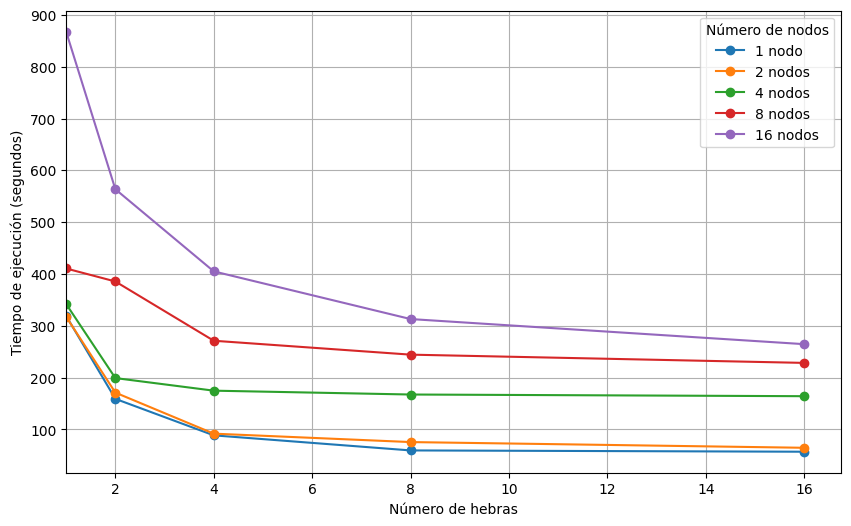
\includegraphics[width=0.8\textwidth]{imagenes/cap5/exploratory_gpu_no-limit_time.png}
    \caption{Gráfica de tiempo de ejecución en función del número de hebras por proceso, permitiendo el uso de la GPU en todos los procesos.}
    \label{fig:exploratory_gpu_no-limit_time}
\end{figure}

Las conclusiones que se pueden extraer de estas gráficas se pueden ver de manera más clara en la tabla \ref{tab:summary_nodes_threads_gpu}, donde se resumen los tiempos de ejecución para todas las combinaciones de procesos y hebras analizadas, tanto con la GPU limitada a un proceso como permitiendo su uso en todos los procesos.

\begin{table}[ht]
    \centering
    \scriptsize
    \setlength{\tabcolsep}{2pt}
    \renewcommand{\arraystretch}{1.1}
    \begin{tabular}{|c|c|c|c|c|}
        \hline
        \textbf{Procesos} & \textbf{Hebras} & \textbf{GPU 1 proceso (s)} & \textbf{GPU todos (s)} & \textbf{Var. (\%)} \\
        \hline
        1                 & 1               & 311.68                     & 319.01                 & 2.35               \\
        1                 & 2               & 163.59                     & 158.94                 & -2.84              \\
        1                 & 4               & 84.49                      & 88.52                  & 4.77               \\
        1                 & 8               & 59.91                      & 59.41                  & -0.83              \\
        1                 & 16              & 56.45                      & 56.91                  & 0.81               \\
        2                 & 1               & 316.92                     & 317.35                 & 0.14               \\
        2                 & 2               & 168.14                     & 170.99                 & 1.70               \\
        2                 & 4               & 90.58                      & 91.78                  & 1.32               \\
        2                 & 8               & 74.30                      & 75.53                  & 1.66               \\
        2                 & 16              & 65.40                      & 64.51                  & -1.36              \\
        4                 & 1               & 322.77                     & 341.95                 & 5.94               \\
        4                 & 2               & 187.98                     & 199.04                 & 5.88               \\
        4                 & 4               & 170.38                     & 174.74                 & 2.56               \\
        4                 & 8               & 163.80                     & 167.31                 & 2.14               \\
        4                 & 16              & 159.22                     & 164.07                 & 3.05               \\
        8                 & 1               & 401.33                     & 410.54                 & 2.29               \\
        8                 & 2               & 393.50                     & 385.47                 & -2.04              \\
        8                 & 4               & 376.68                     & 271.10                 & -28.03             \\
        8                 & 8               & 366.47                     & 244.26                 & -33.35             \\
        8                 & 16              & 363.94                     & 228.34                 & -37.26             \\
        16                & 1               & 869.40                     & 867.50                 & -0.22              \\
        16                & 2               & 628.49                     & 563.51                 & -10.34             \\
        16                & 4               & 496.28                     & 404.98                 & -18.40             \\
        16                & 8               & 427.30                     & 312.94                 & -26.76             \\
        16                & 16              & 400.48                     & 264.49                 & -33.96             \\
        \hline
    \end{tabular}
    \caption{Resumen de tiempos de ejecución para distintas combinaciones de procesos y hebras, comparando el uso de la GPU limitada a un proceso frente a su uso en todos los procesos.}
    \label{tab:summary_nodes_threads_gpu}
\end{table}

Para configuraciones con pocos procesos (1, 2 o 4), la diferencia entre utilizar la GPU en un único proceso o en todos los procesos resulta pequeña y variable. Las variaciones porcentuales oscilan entre valores positivos y negativos, pero en general se mantienen por debajo del 6\%. Esto indica que, en estos escenarios, no existe una ventaja clara ni consistente de emplear la GPU de forma compartida en todos los procesos.

A partir de 8 procesos, la ejecución con la GPU disponible en todos los procesos comienza a mostrar mejoras significativas, especialmente al incrementar el número de hebras. Por ejemplo, con 8 procesos y 16 hebras se observa una reducción del tiempo de ejecución del 37.26\%, mientras que con 16 procesos y 16 hebras la mejora alcanza el 33.96\%. Estas diferencias son consistentes y tienden a aumentar conforme crece el número de procesos y hebras.

En configuraciones con un número elevado de procesos y hebras, la opción de permitir el acceso a la GPU en todos los procesos se presenta como claramente superior, ya que maximiza el aprovechamiento de la capacidad de cómputo distribuido y reduce de manera significativa los tiempos de ejecución.

En resumen, para experimentos pequeños o con pocos procesos ambas opciones resultan comparables. Sin embargo, en experimentos de mayor escala y con configuraciones que involucran un alto número de procesos y hebras, la estrategia más eficiente y recomendable es habilitar el uso de la GPU en todos los procesos.

\subsection{Análisis de los experimentos preliminares}

A partir de los resultados obtenidos, se recomienda fijar el número de subpoblaciones en 8, ya que este valor representa un equilibrio óptimo entre eficiencia, utilización de recursos y escalabilidad en el entorno analizado.

En cuanto al número de hebras, los datos muestran que imponer un límite estricto puede restringir el aprovechamiento total de los recursos, especialmente en configuraciones multiproceso. Por ello, se recomienda no limitar el número de hebras, permitiendo que el sistema utilice tantas como sean necesarias para maximizar el rendimiento.

Respecto al uso de la GPU, los experimentos indican que en configuraciones pequeñas las diferencias entre habilitarla en todos los procesos o solo en uno son mínimas. Sin embargo, en escenarios de mayor escala, habilitar su uso en todos los procesos aporta mejoras sustanciales en el tiempo de ejecución y en la eficiencia global. Por tanto, se establece como criterio general que la GPU esté disponible en todos los procesos.

En conjunto, estas decisiones proporcionan una base sólida y coherente para el diseño de los experimentos posteriores, asegurando que se exploten al máximo los recursos disponibles sin comprometer la comparabilidad de los resultados.

\section{Pruebas monoproceso}

\subsection{Ejecución en Ubuntu en nativo}

\subsubsection{CPU}

En la figura \ref{fig:single-node_ubuntu_cpu_native_time} se muestra el tiempo de ejecución para la configuración de CPU en un único proceso con Ubuntu nativo.

\begin{figure}[ht]
    \centering
    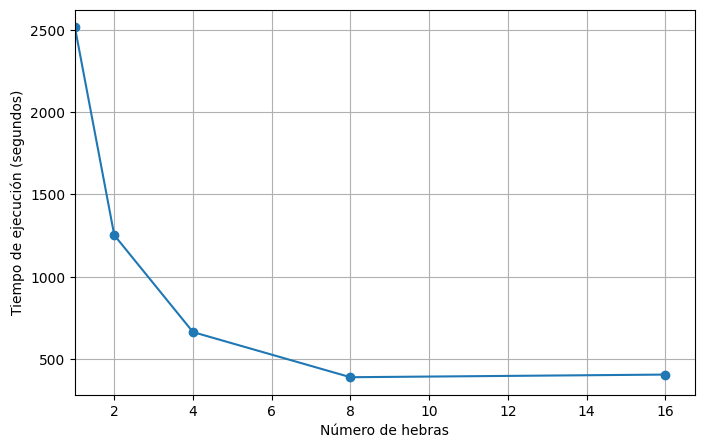
\includegraphics[width=0.8\textwidth]{imagenes/cap5/single-node_ubuntu_cpu_native_time.png}
    \caption{Tiempo de ejecución en función del número de hebras en Ubuntu nativo (CPU).}
    \label{fig:single-node_ubuntu_cpu_native_time}
\end{figure}

En la tabla \ref{tab:single-node_ubuntu_cpu_native} se presentan los tiempos de ejecución y la variación porcentual respecto a una hebra.

\begin{table}[ht]
    \centering
    \begin{tabular}{|c|c|c|}
        \hline
        \textbf{Hebras} & \textbf{Tiempo (s)} & \textbf{$\Delta$\% vs 1 hebra} \\
        \hline
        1               & 2515.21             & 0.00                           \\
        2               & 1253.18             & -50.18                         \\
        4               & 664.69              & -73.57                         \\
        8               & 390.72              & -84.47                         \\
        16              & 406.76              & -83.83                         \\
        \hline
    \end{tabular}
    \caption{Tiempos de ejecución y variación porcentual respecto a una hebra en Ubuntu nativo (CPU).}
    \label{tab:single-node_ubuntu_cpu_native}
\end{table}

El tiempo de ejecución disminuye drásticamente al aumentar el número de hebras, especialmente en el rango de $1$ a $8$ hebras. Con $2$ hebras, el tiempo se reduce prácticamente a la mitad ($-50.18\%$), y con $4$ hebras, a casi una cuarta parte del tiempo original ($-73.57\%$). El mayor beneficio se observa al pasar de $4$ a $8$ hebras, alcanzando una reducción del $84.47\%$ respecto a una hebra. Sin embargo, al incrementar a $16$ hebras, el tiempo de ejecución es ligeramente superior al obtenido con $8$ hebras, lo que sugiere la aparición de saturación o sobrecarga en el sistema. Por tanto, el óptimo se alcanza con $8$ hebras, coincidiendo con el número de núcleos físicos disponibles en el sistema.

En la figura \ref{fig:single-node_ubuntu_cpu_native_cpu} se muestra el porcentaje de uso de CPU en función del número de hebras.

\begin{figure}[ht]
    \centering
    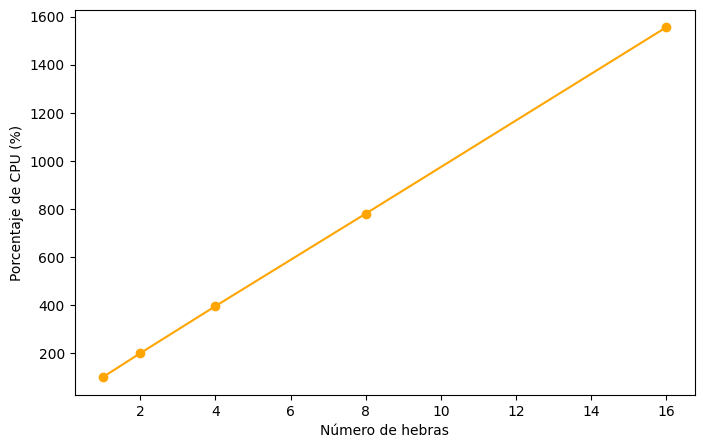
\includegraphics[width=0.8\textwidth]{imagenes/cap5/single-node_ubuntu_cpu_native_cpu.png}
    \caption{Uso de CPU en función del número de hebras en Ubuntu nativo (CPU).}
    \label{fig:single-node_ubuntu_cpu_native_cpu}
\end{figure}

La tabla \ref{tab:single-node_ubuntu_cpu_native_cpu} muestra el porcentaje de uso de CPU alcanzado para cada número de hebras, el máximo teórico posible (calculado como número de hebras por 100\%), y la eficiencia relativa obtenida.

\begin{table}[ht]
    \centering
    \begin{tabular}{|c|c|c|c|}
        \hline
        \textbf{Hebras} & \textbf{CPU (\%)} & \textbf{Max posible CPU (\%)} & \textbf{Efic. CPU (\%)} \\
        \hline
        1               & 99.00             & 100.00                        & 99.00                   \\
        2               & 199.00            & 200.00                        & 99.50                   \\
        4               & 395.00            & 400.00                        & 98.75                   \\
        8               & 780.00            & 800.00                        & 97.50                   \\
        16              & 1556.00           & 1600.00                       & 97.25                   \\
        \hline
    \end{tabular}
    \caption{Porcentaje de uso de CPU y eficiencia en función del número de hebras en Ubuntu nativo (CPU).}
    \label{tab:single-node_ubuntu_cpu_native_cpu}
\end{table}

El uso de CPU aumenta de manera casi lineal conforme se incrementa el número de hebras, lo que evidencia un excelente escalado del paralelismo en la ejecución. La eficiencia de uso de la CPU se mantiene muy elevada en todos los casos, superando el $97\%$, lo que indica que prácticamente se está aprovechando todo el potencial de cómputo disponible. Aunque la eficiencia disminuye ligeramente al aumentar el número de hebras (desde un máximo del $99\%$ hasta un mínimo del $97.25\%$), esta reducción es mínima y esperable, ya que responde a la sobrecarga asociada a la gestión de un mayor número de hilos y a posibles contenciones internas. En conjunto, el sistema demuestra un escalado eficiente hasta $16$ hebras, con una pérdida de eficiencia muy reducida.

Estos resultados evidencian que el entorno monoproceso nativo en Ubuntu gestiona eficazmente el paralelismo y aprovecha bien los recursos de la CPU, mostrando un buen escalado del rendimiento al aumentar el número de hebras.

\subsubsection{CPU + GPU}

En la figura \ref{fig:single-node_ubuntu__gpu_native_time} se muestra el tiempo de ejecución para la configuración de CPU + GPU en un único proceso con Ubuntu nativo.

\begin{figure}[ht]
    \centering
    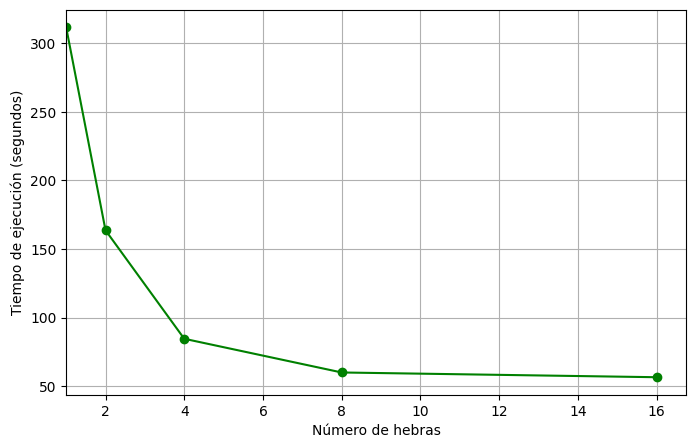
\includegraphics[width=0.8\textwidth]{imagenes/cap5/single-node_ubuntu_gpu_native_time.png}
    \caption{Tiempo de ejecución en función del número de hebras en Ubuntu nativo (CPU + GPU).}
    \label{fig:single-node_ubuntu__gpu_native_time}
\end{figure}

En la tabla \ref{tab:single-node_ubuntu_gpu_native} se presentan los tiempos de ejecución y la variación porcentual respecto a una hebra.

\begin{table}[ht]
    \centering
    \begin{tabular}{|c|c|c|}
        \hline
        \textbf{Hebras} & \textbf{Tiempo (s)} & \textbf{$\Delta$\% vs 1 hebra} \\
        \hline
        1.00            & 311.68              & 0.00                           \\
        2.00            & 163.59              & -47.51                         \\
        4.00            & 84.49               & -72.89                         \\
        8.00            & 59.91               & -80.78                         \\
        16.00           & 56.45               & -81.89                         \\
        \hline
    \end{tabular}
    \caption{Tiempos de ejecución y variación porcentual respecto a una hebra en Ubuntu nativo (CPU + GPU).}
    \label{tab:single-node_ubuntu_gpu_native}
\end{table}

El análisis de los resultados muestra que el tiempo de ejecución disminuye de forma significativa al incrementar el número de hebras, especialmente en el rango de $1$ a $4$ hebras, donde se alcanza una reducción del $72.89\%$. La mayor ganancia relativa se produce al pasar de $1$ a $2$ hebras ($-47.51\%$) y de $2$ a $4$ hebras ($-25.38\%$ adicional). Sin embargo, a partir de $8$ hebras, la mejora es marginal: el tiempo de ejecución solo disminuye de $59.91\,s$ a $56.45\,s$ al pasar de $8$ a $16$ hebras, lo que supone apenas un $1.11\%$ adicional. Esto indica que el sistema alcanza un punto óptimo de rendimiento con $8$ hebras, y que a partir de ese valor se observa una saturación en la eficiencia de la paralelización. En conjunto, la combinación CPU + GPU proporciona una aceleración notable, pero la eficiencia se estabiliza a partir de cierto número de hebras, reflejando el límite práctico de paralelismo efectivo en el entorno analizado.

\subsubsection{Comparativa CPU vs CPU + GPU}

En la figura \ref{fig:single-node_ubuntu_cpu_vs_gpu_native_time} se muestra una comparativa del tiempo de ejecución entre las configuraciones de CPU y CPU + GPU en un único proceso con Ubuntu nativo.

\begin{figure}[ht]
    \centering
    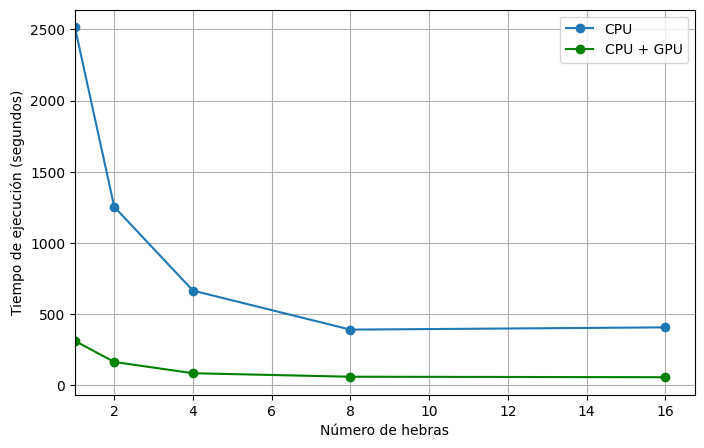
\includegraphics[width=0.8\textwidth]{imagenes/cap5/single-node_ubuntu_cpu_vs_gpu_native_time.png}
    \caption{Comparativa de tiempo de ejecución entre CPU y CPU + GPU en función del número de hebras en Ubuntu nativo.}
    \label{fig:single-node_ubuntu_cpu_vs_gpu_native_time}
\end{figure}

En la tabla \ref{tab:single-node_ubuntu_cpu_vs_gpu_native} se presentan los tiempos de ejecución para ambas configuraciones y la variación porcentual entre ellas.

\begin{table}[ht]
    \centering
    \begin{tabular}{|c|c|c|c|}
        \hline
        \textbf{Hebras} & \textbf{Tiempo CPU (s)} & \textbf{Tiempo CPU+GPU (s)} & \textbf{Var. (\%)} \\
        \hline
        1               & 2515.21                 & 311.68                      & -87.61             \\
        2               & 1253.18                 & 163.59                      & -86.95             \\
        4               & 664.69                  & 84.49                       & -87.29             \\
        8               & 390.72                  & 59.91                       & -84.67             \\
        16              & 406.76                  & 56.45                       & -86.12             \\
        \hline
    \end{tabular}
    \caption{Comparativa de tiempos de ejecución y variación porcentual entre CPU y CPU+GPU en Ubuntu nativo.}
    \label{tab:single-node_ubuntu_cpu_vs_gpu_native}
\end{table}

El análisis de los resultados muestra que el uso de GPU reduce el tiempo de ejecución entre un $84\%$ y un $88\%$ respecto a la ejecución únicamente en CPU, independientemente del número de hebras empleadas. La mejora relativa se mantiene estable al aumentar el paralelismo, lo que indica que la GPU aporta un beneficio constante y no dependiente del número de hilos de CPU utilizados. Además, mientras que en la configuración solo CPU el tiempo de ejecución deja de mejorar al pasar de $8$ a $16$ hebras (e incluso empeora ligeramente), en la configuración CPU+GPU la mejora es marginal pero consistente. En conjunto, la incorporación de GPU resulta altamente beneficiosa, acelerando el procesamiento en torno al $85\%$ en todos los escenarios analizados.

\subsection{Ejecución en contenedores de Ubuntu}
\subsubsection{CPU}

En la figura \ref{fig:single-node_ubuntu_docker_time} se muestra el tiempo de ejecución para la configuración de CPU en un único proceso con contenedores de Ubuntu.

\begin{figure}[ht]
    \centering
    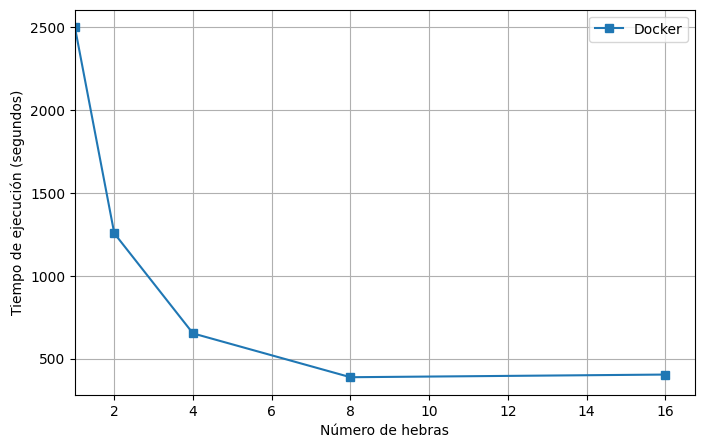
\includegraphics[width=0.8\textwidth]{imagenes/cap5/single-node_ubuntu_docker_time.png}
    \caption{Tiempo de ejecución en un único proceso con contenedores de Ubuntu (CPU).}
    \label{fig:single-node_ubuntu_docker_time}
\end{figure}

En la tabla \ref{tab:single-node_ubuntu_docker} se presentan los tiempos de ejecución y la variación porcentual respecto a una hebra.

\begin{table}[ht]
    \centering
    \begin{tabular}{|c|c|c|}
        \hline
        \textbf{Hebras} & \textbf{Tiempo (s)} & \textbf{$\Delta$\% vs 1 hebra} \\
        \hline
        1               & 2499.09             & 0.00                           \\
        2               & 1255.95             & -49.74                         \\
        4               & 652.33              & -73.90                         \\
        8               & 388.04              & -84.47                         \\
        16              & 404.09              & -83.83                         \\
        \hline
    \end{tabular}
    \caption{Tiempos de ejecución y variación porcentual respecto a una hebra en contenedores de Ubuntu (CPU).}
    \label{tab:single-node_ubuntu_docker}
\end{table}

El tiempo de ejecución disminuye significativamente al aumentar el número de hebras, especialmente al pasar de 1 a 8 hebras, donde la reducción alcanza el 84.47\%.

La mayor ganancia relativa se obtiene al pasar de 1 a 2 hebras (-49.74\%) y de 2 a 4 hebras (-48.16\% adicional), mostrando una buena escalabilidad inicial.

A partir de 8 hebras, la mejora se estabiliza y el rendimiento apenas varía, e incluso con 16 hebras el tiempo de ejecución es ligeramente superior al de 8 hebras, lo que indica que se alcanza un límite de paralelización eficiente.

Estos resultados sugieren que, en este entorno, el uso de más de 8 hebras no aporta beneficios significativos y puede incluso generar sobrecarga, por lo que 8 hebras representa el punto óptimo de eficiencia para la ejecución en contenedores de Ubuntu con CPU.

En la figura \ref{fig:single-node_ubuntu_podman_time} se muestra el tiempo de ejecución para la configuración de CPU en un único proceso con contenedores de Ubuntu gestionados por \textit{Podman}.

\begin{figure}[ht]
    \centering
    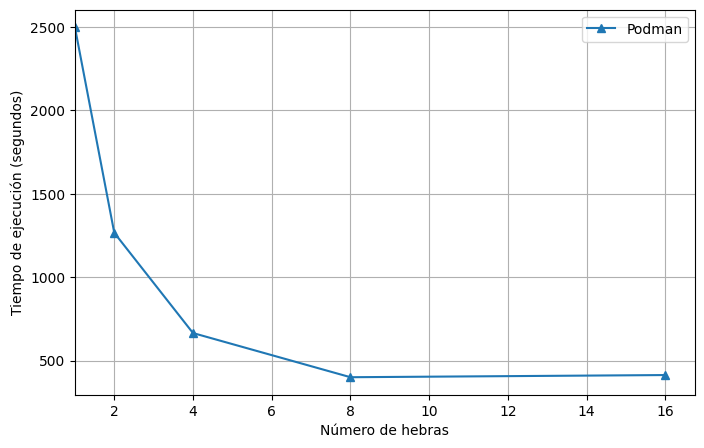
\includegraphics[width=0.8\textwidth]{imagenes/cap5/single-node_ubuntu_podman_time.png}
    \caption{Tiempo de ejecución en un único proceso con contenedores de Ubuntu gestionados por \textit{Podman} (CPU).}
    \label{fig:single-node_ubuntu_podman_time}
\end{figure}

En la tabla \ref{tab:single-node_ubuntu_podman} se presentan los tiempos de ejecución y la variación porcentual respecto a una hebra.

\begin{table}[ht]
    \centering
    \begin{tabular}{|c|c|c|}
        \hline
        \textbf{Hebras} & \textbf{Tiempo (s)} & \textbf{$\Delta$\% vs 1 hebra} \\
        \hline
        1               & 2499.16             & 0.00                           \\
        2               & 1266.51             & -49.32                         \\
        4               & 665.38              & -73.38                         \\
        8               & 400.51              & -83.97                         \\
        16              & 413.53              & -83.45                         \\
        \hline
    \end{tabular}
    \caption{Tiempos de ejecución y variación porcentual respecto a una hebra en contenedores de Ubuntu gestionados por \textit{Podman} (CPU).}
    \label{tab:single-node_ubuntu_podman}
\end{table}

El tiempo de ejecución disminuye de forma considerable al aumentar el número de hebras, especialmente entre 1 y 8 hebras, donde la reducción alcanza el 83.97\%.

La mayor mejora relativa se observa al pasar de 1 a 2 hebras (-49.32\%) y de 2 a 4 hebras (-47.97\% adicional), lo que indica una buena escalabilidad inicial.

A partir de 8 hebras, la reducción en el tiempo de ejecución se estabiliza y el beneficio adicional es mínimo; con 16 hebras, el tiempo incluso aumenta ligeramente respecto a 8 hebras, lo que sugiere que se alcanza el límite de paralelización eficiente.

Estos resultados muestran que, en este entorno con \textit{Podman} y CPU, el uso óptimo se encuentra en torno a 8 hebras, ya que aumentar más allá de este valor no aporta mejoras significativas y puede generar sobrecarga.

\subsubsection{CPU + GPU}

En la figura \ref{fig:single-node_ubuntu_docker_gpu_time} se muestra el tiempo de ejecución para la configuración de CPU + GPU en un único proceso con contenedores de Ubuntu.

\begin{figure}[ht]
    \centering
    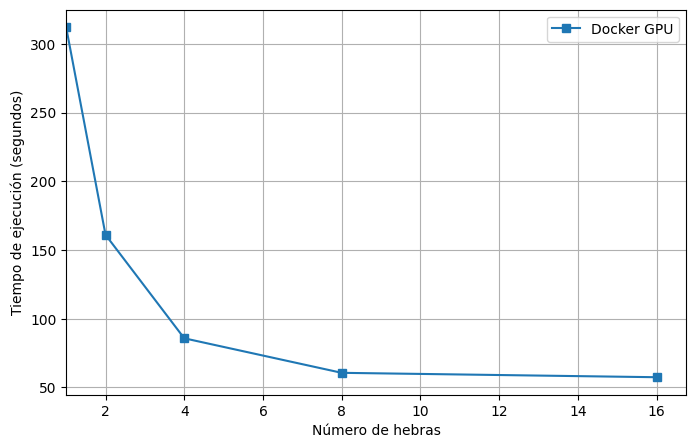
\includegraphics[width=0.8\textwidth]{imagenes/cap5/single-node_ubuntu_docker_gpu_time.png}
    \caption{Tiempo de ejecución en un único proceso con contenedores de Ubuntu (CPU + GPU).}
    \label{fig:single-node_ubuntu_docker_gpu_time}
\end{figure}

En la tabla \ref{tab:single-node_ubuntu_docker_gpu} se presentan los tiempos de ejecución y la variación porcentual respecto a una hebra.

\begin{table}[ht]
    \centering
    \begin{tabular}{|c|c|c|}
        \hline
        \textbf{Hebras} & \textbf{Tiempo (s)} & \textbf{$\Delta$\% vs 1 hebra} \\
        \hline
        1               & 312.18              & 0.00                           \\
        2               & 161.10              & -48.40                         \\
        4               & 85.78               & -72.52                         \\
        8               & 60.65               & -80.57                         \\
        16              & 57.45               & -81.60                         \\
        \hline
    \end{tabular}
    \caption{Tiempos de ejecución y variación porcentual respecto a una hebra en contenedores de Ubuntu (CPU + GPU).}
    \label{tab:single-node_ubuntu_docker_gpu}
\end{table}

El uso combinado de CPU y GPU en contenedores de Ubuntu permite una variación muy significativa en los tiempos de ejecución al aumentar el número de hebras, alcanzando una disminución del 81.60\% con 16 hebras respecto a la ejecución con una sola hebra.

La mayor ganancia relativa se observa al pasar de 1 a 2 hebras (-48.40\%) y de 2 a 4 hebras (-24.12\% adicional), lo que indica una buena escalabilidad inicial.

A partir de 8 hebras, la mejora se estabiliza y el beneficio adicional es marginal; el tiempo de ejecución con 16 hebras es solo ligeramente menor que con 8 hebras.

Estos resultados muestran que, en este entorno, la combinación de CPU y GPU permite aprovechar eficientemente el paralelismo hasta 8 hebras, siendo el punto óptimo de eficiencia, ya que aumentar más allá de este valor aporta mejoras muy pequeñas.

En la figura \ref{fig:single-node_ubuntu_podman_gpu_time} se muestra el tiempo de ejecución para la configuración de CPU + GPU en un único proceso con contenedores de Ubuntu gestionados por \textit{Podman}.

\begin{figure}[ht]
    \centering
    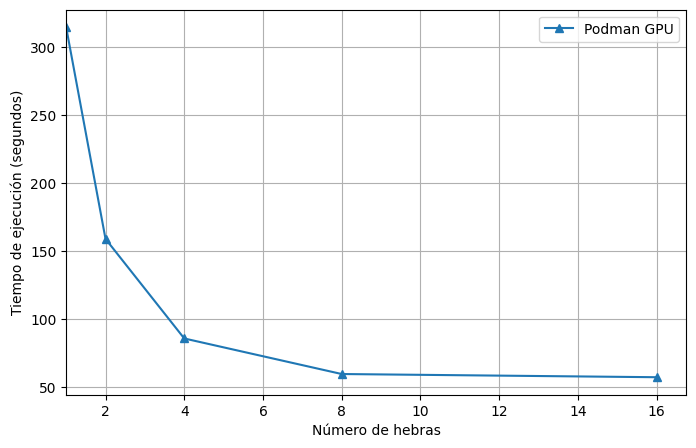
\includegraphics[width=0.8\textwidth]{imagenes/cap5/single-node_ubuntu_podman_gpu_time.png}
    \caption{Tiempo de ejecución en un único proceso con contenedores de Ubuntu gestionados por \textit{Podman} (CPU + GPU).}
    \label{fig:single-node_ubuntu_podman_gpu_time}
\end{figure}

En la tabla \ref{tab:single-node_ubuntu_podman_gpu} se presentan los tiempos de ejecución y la variación porcentual respecto a una hebra.

\begin{table}[ht]
    \centering
    \begin{tabular}{|c|c|c|}
        \hline
        \textbf{Hebras} & \textbf{Tiempo (s)} & \textbf{$\Delta$\% vs 1 hebra} \\
        \hline
        1               & 314.51              & 0.00                           \\
        2               & 158.84              & -49.50                         \\
        4               & 85.62               & -72.78                         \\
        8               & 59.47               & -81.09                         \\
        16              & 57.12               & -81.84                         \\
        \hline
    \end{tabular}
    \caption{Tiempos de ejecución y variación porcentual respecto a una hebra en contenedores de Ubuntu gestionados por \textit{Podman} (CPU + GPU).}
    \label{tab:single-node_ubuntu_podman_gpu}
\end{table}

El tiempo de ejecución disminuye drásticamente al aumentar el número de hebras, alcanzando una reducción del 81.84\% con 16 hebras respecto a la ejecución con una sola hebra.

La mayor mejora relativa se observa al pasar de 1 a 2 hebras (-49.50\%) y de 2 a 4 hebras (-23.28\% adicional), lo que indica una excelente escalabilidad inicial.

A partir de 8 hebras, la reducción en el tiempo de ejecución se estabiliza y el beneficio adicional es muy pequeño; el tiempo con 16 hebras es solo ligeramente menor que con 8 hebras.

Estos resultados muestran que, en este entorno con \textit{Podman} y CPU+GPU, el uso óptimo se encuentra en torno a 8 hebras, ya que aumentar más allá de este valor no aporta mejoras significativas y puede generar sobrecarga.

\subsubsection{Comparativa contenedores vs nativo}

En la figura \ref{fig:single-node_ubuntu_container_vs_native_time} se muestra una comparativa del tiempo de ejecución entre las configuraciones nativas y en contenedores de Ubuntu para CPU.

\begin{figure}[ht]
    \centering
    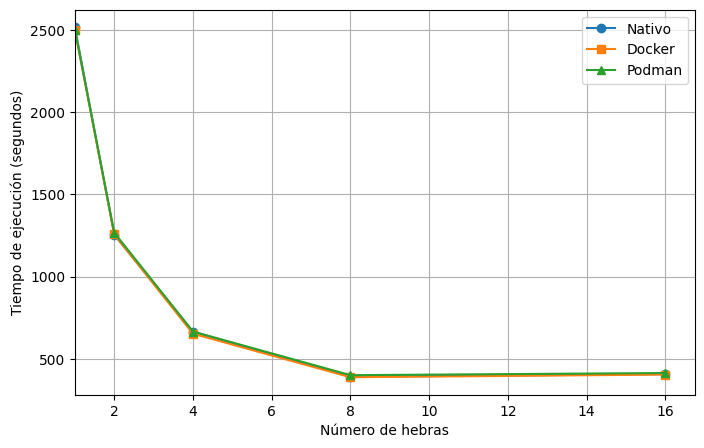
\includegraphics[width=0.8\textwidth]{imagenes/cap5/single-node_ubuntu_container_vs_native_time.png}
    \caption{Comparativa de tiempo de ejecución entre nativo y contenedores de Ubuntu en función del número de hebras, para CPU.}
    \label{fig:single-node_ubuntu_container_vs_native_time}
\end{figure}

En la tabla \ref{tab:single-node_ubuntu_container_vs_native} se presentan los tiempos de ejecución para ambas configuraciones y la variación porcentual entre ellas.

\begin{table}[ht]
    \centering
    \begin{tabular}{|c|c|c|c|c|c|}
        \hline
        \textbf{Hebras} & \textbf{Nativo (s)} & \textbf{\textit{Docker} (s)} & \textbf{\textit{Docker} $\Delta$\%} & \textbf{\textit{Podman} (s)} & \textbf{\textit{Podman} $\Delta$\%} \\
        \hline
        1.00            & 2515.21             & 2499.09                      & -0.64                               & 2499.16                      & -0.64                               \\
        2.00            & 1253.18             & 1255.95                      & 0.22                                & 1266.51                      & 1.06                                \\
        4.00            & 664.69              & 652.33                       & -1.86                               & 665.38                       & 0.10                                \\
        8.00            & 390.72              & 388.04                       & -0.69                               & 400.51                       & 2.51                                \\
        16.00           & 406.76              & 404.09                       & -0.66                               & 413.53                       & 1.66                                \\
        \hline
    \end{tabular}
    \caption{Comparativa de tiempos de ejecución entre nativo, \textit{Docker} y \textit{Podman} en función del número de hebras y variación porcentual respecto a nativo (CPU, monoproceso).}
    \label{tab:single-node_ubuntu_container_vs_native}
\end{table}

La tabla compara los tiempos de ejecución entre los entornos nativo, \textit{Docker} y \textit{Podman} en un escenario monoproceso utilizando únicamente CPU y diferentes números de hebras, mostrando además la variación porcentual de los contenedores respecto al entorno nativo. Con una hebra, tanto \textit{Docker} como \textit{Podman} presentan tiempos de ejecución ligeramente inferiores al nativo, con una reducción del 0.64\%, lo que indica que la sobrecarga de los contenedores es prácticamente inexistente en este caso. Al aumentar a dos hebras, \textit{Docker} muestra un incremento mínimo del 0.22\% y \textit{Podman} del 1.06\%, lo que sugiere que la eficiencia de los contenedores se mantiene muy próxima a la del entorno nativo. Con cuatro hebras, \textit{Docker} logra una mejora del 1.86\% respecto al nativo, mientras que \textit{Podman} se mantiene prácticamente igual, lo que podría estar relacionado con pequeñas diferencias en la gestión de recursos internos. Al incrementar el número de hebras a ocho y dieciséis, las diferencias siguen siendo muy reducidas, con \textit{Docker} mostrando ligeras mejoras y \textit{Podman} presentando incrementos moderados, pero siempre dentro de un margen muy estrecho. En conjunto, estos resultados evidencian que el uso de contenedores en un entorno monoproceso y CPU no introduce penalizaciones significativas en el rendimiento y, en algunos casos, puede incluso aportar pequeñas mejoras, confirmando la viabilidad de \textit{Docker} y \textit{Podman} para la ejecución eficiente de aplicaciones paralelas en este tipo de escenarios.

La figura \ref{fig:single-node_ubuntu_container_vs_native_gpu_time} muestra una comparativa del tiempo de ejecución entre las configuraciones nativas y en contenedores de Ubuntu para CPU + GPU.

\begin{figure}[ht]
    \centering
    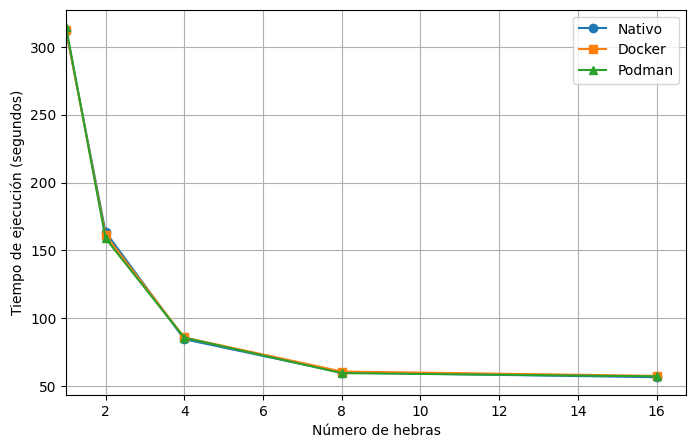
\includegraphics[width=0.8\textwidth]{imagenes/cap5/single-node_ubuntu_container_vs_native_gpu_time.png}
    \caption{Comparativa de tiempo de ejecución entre nativo y contenedores de Ubuntu en función del número de hebras, para CPU + GPU.}
    \label{fig:single-node_ubuntu_container_vs_native_gpu_time}
\end{figure}

En la tabla \ref{tab:single-node_ubuntu_container_vs_native_gpu} se presentan los tiempos de ejecución para ambas configuraciones y la variación porcentual entre ellas.

\begin{table}[ht]
    \centering
    \small
    \setlength{\tabcolsep}{4pt}
    \renewcommand{\arraystretch}{1.1}
    \begin{tabular}{|c|c|c|c|c|c|}
        \hline
        \textbf{Hebras} & \textbf{Nativo (s)} & \textbf{\textit{Docker} (s)} & \textbf{\textit{Docker} $\Delta$\%} & \textbf{\textit{Podman} (s)} & \textbf{\textit{Podman} $\Delta$\%} \\
        \hline
        1.00            & 2515.21             & 2499.09                      & -0.64                               & 2499.16                      & -0.64                               \\
        2.00            & 1253.18             & 1255.95                      & 0.22                                & 1266.51                      & 1.06                                \\
        4.00            & 664.69              & 652.33                       & -1.86                               & 665.38                       & 0.10                                \\
        8.00            & 390.72              & 388.04                       & -0.69                               & 400.51                       & 2.51                                \\
        16.00           & 406.76              & 404.09                       & -0.66                               & 413.53                       & 1.66                                \\
        \hline
    \end{tabular}
    \caption{Comparativa de tiempos de ejecución entre nativo, \textit{Docker} y \textit{Podman} en función del número de hebras y variación porcentual respecto a nativo (CPU + GPU, monoproceso).}
    \label{tab:single-node_ubuntu_container_vs_native_gpu}
\end{table}

La tabla compara los tiempos de ejecución entre los entornos nativo, \textit{Docker} y \textit{Podman} en un escenario monoproceso con CPU + GPU, mostrando también la variación porcentual de los contenedores respecto al entorno nativo para diferentes números de hebras. Los resultados indican que las diferencias de rendimiento entre la ejecución nativa y en contenedores son mínimas. Con una hebra, tanto \textit{Docker} como \textit{Podman} presentan tiempos de ejecución ligeramente inferiores al nativo (reducción del 0.64\%), lo que sugiere que la sobrecarga de los contenedores es prácticamente inexistente en este caso. Al aumentar el número de hebras, las diferencias siguen siendo muy pequeñas: \textit{Docker} oscila entre ligeras mejoras y pequeñas penalizaciones (máximo -1.86\% y 0.22\%), mientras que \textit{Podman} muestra valores similares, con variaciones que no superan el 2.51\%. En conjunto, estos resultados evidencian que el uso de contenedores \textit{Docker} o \textit{Podman} en un entorno monoproceso con CPU + GPU no introduce penalizaciones significativas en el rendimiento respecto a la ejecución nativa, confirmando la viabilidad de ambas tecnologías para la ejecución eficiente de aplicaciones paralelas en este tipo de escenarios.

\subsection{Ejecución en contenedores de Windows}
\subsubsection{CPU}

En la figura \ref{fig:single-node_windows_docker_time} se muestra el tiempo de ejecución para la configuración de CPU en un único proceso con \textit{Docker} en Windows.

\begin{figure}[ht]
    \centering
    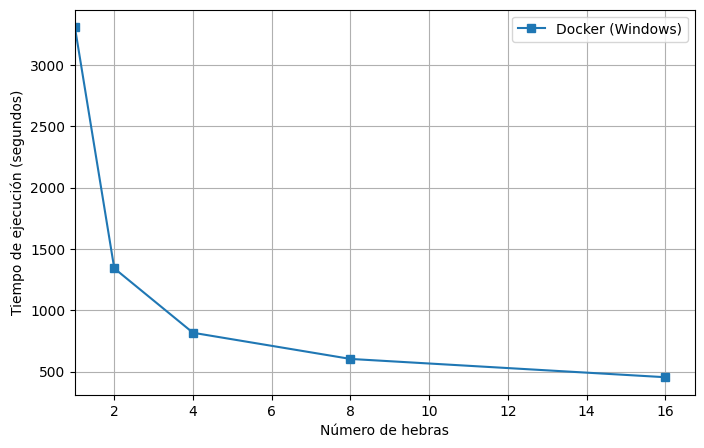
\includegraphics[width=0.8\textwidth]{imagenes/cap5/single-node_windows_docker_time.png}
    \caption{Tiempo de ejecución en un único proceso con \textit{Docker} en Windows (CPU).}
    \label{fig:single-node_windows_docker_time}
\end{figure}

En la tabla \ref{tab:single-node_windows_docker_time} se presentan los tiempos de ejecución y la reducción porcentual respecto a una hebra.

\begin{table}[ht]
    \centering
    \begin{tabular}{|c|c|c|}
        \hline
        \textbf{Hebras} & \textbf{Tiempo (s)} & \textbf{$\Delta$\% vs 1 hebra} \\
        \hline
        1.00            & 3308.08             & 0.00                           \\
        2.00            & 1341.41             & -59.45                         \\
        4.00            & 816.06              & -75.33                         \\
        8.00            & 602.60              & -81.78                         \\
        16.00           & 453.44              & -86.29                         \\
        \hline
    \end{tabular}
    \caption{Tiempos de ejecución y reducción porcentual respecto a una hebra en \textit{Docker} sobre Windows (CPU).}
    \label{tab:single-node_windows_docker_time}
\end{table}

El tiempo de ejecución disminuye de forma significativa al aumentar el número de hebras, alcanzando una reducción del 86.29\% con 16 hebras respecto a la ejecución con una sola hebra.

La mayor mejora relativa se observa al pasar de 1 a 2 hebras (-59.45\%) y de 2 a 4 hebras (-39.46\% adicional), lo que indica una excelente escalabilidad inicial.

A medida que se incrementa el número de hebras, la reducción en el tiempo de ejecución se mantiene, aunque con beneficios marginales decrecientes a partir de 8 hebras.

Estos resultados muestran que, en \textit{Docker} sobre Windows (CPU), el uso de múltiples hebras es muy eficiente y permite aprovechar el paralelismo, siendo recomendable utilizar el mayor número de hebras posible para minimizar el tiempo de ejecución.

En la figura \ref{fig:single-node_windows_podman_time} se muestra el tiempo de ejecución para la configuración de CPU en un único proceso con \textit{Podman} en Windows.

\begin{figure}[ht]
    \centering
    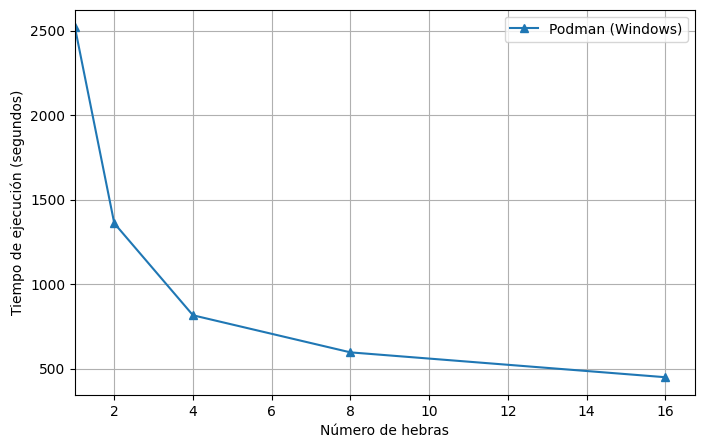
\includegraphics[width=0.8\textwidth]{imagenes/cap5/single-node_windows_podman_time.png}
    \caption{Tiempo de ejecución en un único proceso con \textit{Podman} en Windows (CPU).}
    \label{fig:single-node_windows_podman_time}
\end{figure}

En la tabla \ref{tab:single-node_windows_podman_time} se presentan los tiempos de ejecución y la reducción porcentual respecto a una hebra.

\begin{table}[ht]
    \centering
    \begin{tabular}{|c|c|c|}
        \hline
        \textbf{Hebras} & \textbf{Tiempo (s)} & \textbf{$\Delta$\% vs 1 hebra} \\
        \hline
        1.00            & 2520.21             & 0.00                           \\
        2.00            & 1359.69             & -46.05                         \\
        4.00            & 815.04              & -67.66                         \\
        8.00            & 595.54              & -76.37                         \\
        16.00           & 448.43              & -82.21                         \\
        \hline
    \end{tabular}
    \caption{Tiempos de ejecución y reducción porcentual respecto a una hebra en \textit{Podman} sobre Windows (CPU).}
    \label{tab:single-node_windows_podman_time}
\end{table}

El tiempo de ejecución disminuye notablemente al aumentar el número de hebras, alcanzando una reducción del 82.21\% con 16 hebras respecto a una sola hebra.

La mayor mejora relativa se observa al pasar de 1 a 2 hebras (-46.05\%) y de 2 a 4 hebras (-21.61\% adicional), lo que indica una buena escalabilidad inicial.

A partir de 8 hebras, la reducción en el tiempo de ejecución continúa, aunque los beneficios adicionales son menores, mostrando una tendencia a estabilizarse.

Estos resultados indican que, en \textit{Podman} sobre Windows (CPU), el uso de múltiples hebras es eficiente y permite aprovechar el paralelismo, siendo recomendable utilizar el mayor número de hebras posible para reducir el tiempo de ejecución, aunque las ganancias adicionales disminuyen a partir de 8 hebras.

\subsubsection{CPU + GPU}

En la figura \ref{fig:single-node_windows_docker_gpu_time} se muestra el tiempo de ejecución para la configuración de CPU + GPU en un único proceso con contenedores de Ubuntu.

\begin{figure}[ht]
    \centering
    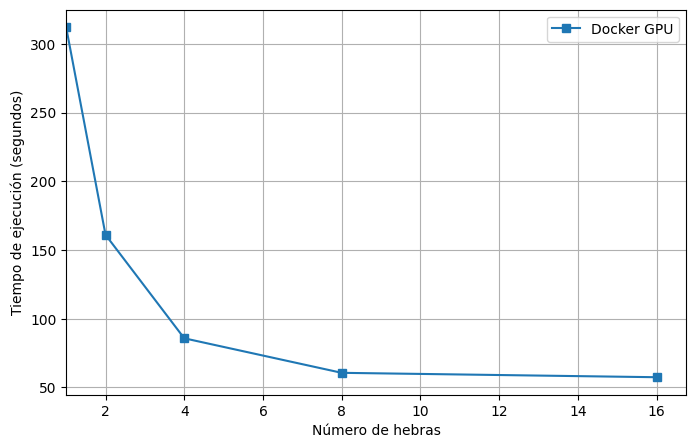
\includegraphics[width=0.8\textwidth]{imagenes/cap5/single-node_ubuntu_docker_gpu_time.png}
    \caption{Tiempo de ejecución en un único proceso con contenedores de Windows (CPU + GPU).}
    \label{fig:single-node_windows_docker_gpu_time}
\end{figure}

En la tabla \ref{tab:single-node_windows_docker_gpu} se presentan los tiempos de ejecución y la variación porcentual respecto a una hebra.

\begin{table}[ht]
    \centering
    \begin{tabular}{|c|c|c|}
        \hline
        \textbf{Hebras} & \textbf{Tiempo (s)} & \textbf{$\Delta$\% vs 1 hebra} \\
        \hline
        1               & 423.56              & 0.00                           \\
        2               & 226.73              & -46.40                         \\
        4               & 128.93              & -69.52                         \\
        8               & 90.65               & -78.57                         \\
        16              & 82.06               & -80.60                         \\
        \hline
    \end{tabular}
    \caption{Tiempos de ejecución y variación porcentual respecto a una hebra en contenedores de Windows (CPU + GPU).}
    \label{tab:single-node_windows_docker_gpu}
\end{table}

El tiempo de ejecución disminuye de forma notable al aumentar el número de hebras, alcanzando una reducción del 80.60\% con 16 hebras respecto a una sola hebra.

La mayor mejora relativa se observa al pasar de 1 a 2 hebras (-46.40\%) y de 2 a 4 hebras (-23.12\% adicional), lo que indica una buena escalabilidad inicial.

A partir de 8 hebras, la reducción en el tiempo de ejecución se estabiliza, con beneficios adicionales menores al incrementar a 16 hebras.

Estos resultados muestran que, en contenedores de Windows con CPU+GPU, el uso de múltiples hebras es eficiente y permite aprovechar el paralelismo, siendo recomendable utilizar al menos 8 hebras para obtener la mayor parte de la mejora, ya que las ganancias adicionales más allá de ese punto son limitadas.

En la figura \ref{fig:single-node_windows_podman_gpu_time} se muestra el tiempo de ejecución para la configuración de CPU + GPU en un único proceso con contenedores de Windows gestionados por \textit{Podman}.

\begin{figure}[ht]
    \centering
    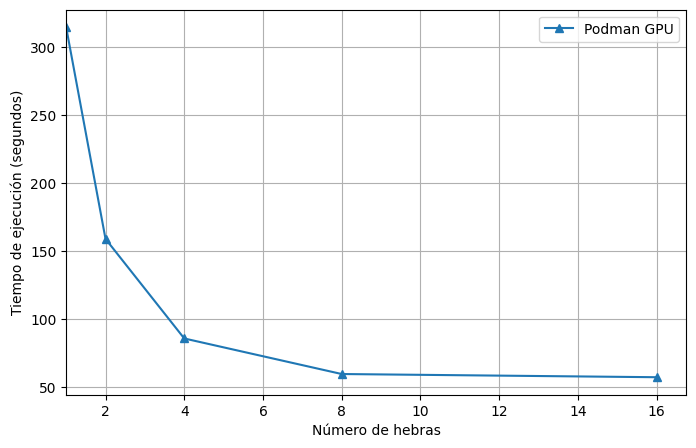
\includegraphics[width=0.8\textwidth]{imagenes/cap5/single-node_ubuntu_podman_gpu_time.png}
    \caption{Tiempo de ejecución en un único proceso con contenedores de Windows gestionados por \textit{Podman} (CPU + GPU).}
    \label{fig:single-node_windows_podman_gpu_time}
\end{figure}

En la tabla \ref{tab:single-node_windows_podman_gpu} se presentan los tiempos de ejecución y la variación porcentual respecto a una hebra.

\begin{table}[ht]
    \centering
    \begin{tabular}{|c|c|c|}
        \hline
        \textbf{Hebras} & \textbf{Tiempo (s)} & \textbf{$\Delta$\% vs 1 hebra} \\
        \hline
        1               & 426.56              & 0.00                           \\
        2               & 226.73              & -48.40                         \\
        4               & 123.93              & -68.15                         \\
        8               & 95.65               & -79.57                         \\
        16              & 84.06               & -81.05                         \\
        \hline
    \end{tabular}
    \caption{Tiempos de ejecución y variación porcentual respecto a una hebra en contenedores de Windows (CPU + GPU).}
    \label{tab:single-node_windows_podman_gpu}
\end{table}

El tiempo de ejecución disminuye considerablemente al aumentar el número de hebras, alcanzando una reducción del 81.05\% con 16 hebras respecto a una sola hebra.

La mayor mejora relativa se observa al pasar de 1 a 2 hebras (-48.40\%) y de 2 a 4 hebras (-19.75\% adicional), lo que indica una buena escalabilidad inicial.

A partir de 8 hebras, la reducción en el tiempo de ejecución se estabiliza, con beneficios adicionales menores al incrementar a 16 hebras.

Estos resultados muestran que, en contenedores de Windows con CPU+GPU, el uso de múltiples hebras es eficiente y permite aprovechar el paralelismo, siendo recomendable utilizar al menos 8 hebras para obtener la mayor parte de la mejora, ya que las ganancias adicionales más allá de ese punto son limitadas.

\subsection{Ejecución en contenedores de MacOS}
\subsubsection{CPU}

En la figura \ref{fig:single-node_mac_docker_time} se muestra el tiempo de ejecución para la configuración de CPU en un único proceso con \textit{Docker} en MacOS.

\begin{figure}[ht]
    \centering
    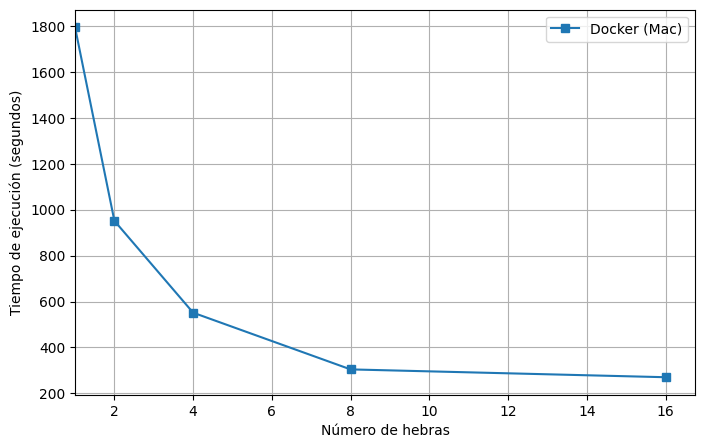
\includegraphics[width=0.8\textwidth]{imagenes/cap5/single-node_mac_docker_time.png}
    \caption{Tiempo de ejecución en un único proceso con \textit{Docker} en MacOS (CPU).}
    \label{fig:single-node_mac_docker_time}
\end{figure}

En la tabla \ref{tab:single-node_mac_docker_time} se presentan los tiempos de ejecución y la reducción porcentual respecto a una hebra.

\begin{table}[ht]
    \centering
    \begin{tabular}{|c|c|c|}
        \hline
        \textbf{Hebras} & \textbf{Tiempo (s)} & \textbf{$\Delta$\% vs 1 hebra} \\
        \hline
        1.00            & 1794.98             & 0.00                           \\
        2.00            & 951.56              & -46.99                         \\
        4.00            & 551.41              & -69.28                         \\
        8.00            & 304.35              & -83.04                         \\
        16.00           & 270.25              & -84.94                         \\
        \hline
    \end{tabular}
    \caption{Tiempos de ejecución y reducción porcentual respecto a una hebra en \textit{Docker} sobre MacOS (CPU).}
    \label{tab:single-node_mac_docker_time}
\end{table}

El tiempo de ejecución disminuye considerablemente al aumentar el número de hebras, alcanzando una reducción del 84.94\% con 16 hebras respecto a una sola hebra.

La mayor mejora relativa se observa al pasar de 1 a 2 hebras (-46.99\%) y de 2 a 4 hebras (-22.29\% adicional), lo que indica una buena escalabilidad inicial.

A partir de 8 hebras, la reducción en el tiempo de ejecución se estabiliza, con beneficios adicionales menores al incrementar a 16 hebras.

Estos resultados muestran que, en \textit{Docker} sobre MacOS(CPU), el uso de múltiples hebras es eficiente y permite aprovechar el paralelismo, siendo recomendable utilizar el mayor número de hebras posible para minimizar el tiempo de ejecución, aunque las ganancias adicionales disminuyen a partir de 8 hebras.

En la figura \ref{fig:single-node_mac_podman_time} se muestra el tiempo de ejecución para la configuración de CPU en un único proceso con \textit{Podman} en MacOS.

\begin{figure}[ht]
    \centering
    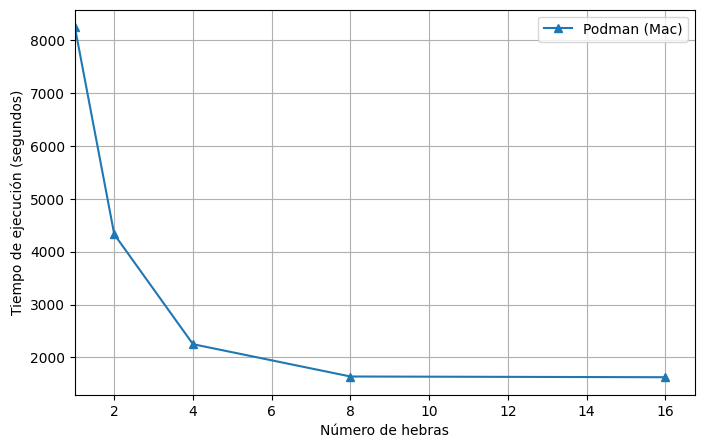
\includegraphics[width=0.8\textwidth]{imagenes/cap5/single-node_mac_podman_time.png}
    \caption{Tiempo de ejecución en un único proceso con \textit{Podman} en MacOS (CPU).}
    \label{fig:single-node_mac_podman_time}
\end{figure}

En la tabla \ref{tab:single-node_mac_podman_time} se presentan los tiempos de ejecución y la reducción porcentual respecto a una hebra.

\begin{table}[ht]
    \centering
    \begin{tabular}{|c|c|c|}
        \hline
        \textbf{Hebras} & \textbf{Tiempo (s)} & \textbf{$\Delta$\% vs 1 hebra} \\
        \hline
        1.00            & 8247.00             & 0.00                           \\
        2.00            & 4328.00             & -47.52                         \\
        4.00            & 2250.20             & -72.71                         \\
        8.00            & 1638.79             & -80.13                         \\
        16.00           & 1625.19             & -80.29                         \\
        \hline
    \end{tabular}
    \caption{Tiempos de ejecución y reducción porcentual respecto a una hebra en \textit{Podman} sobre MacOS(CPU).}
    \label{tab:single-node_mac_podman_time}
\end{table}

El tiempo de ejecución disminuye de forma muy significativa al aumentar el número de hebras, alcanzando una reducción del 80.29\% con 16 hebras respecto a una sola hebra.

La mayor mejora relativa se observa al pasar de 1 a 2 hebras (-47.52\%) y de 2 a 4 hebras (-25.19\% adicional), lo que indica una buena escalabilidad inicial.

A partir de 8 hebras, la reducción en el tiempo de ejecución se estabiliza, con beneficios adicionales mínimos al incrementar a 16 hebras (solo -0.16\% respecto a 8 hebras).

Estos resultados muestran que, en \textit{Podman} sobre MacOS(CPU), el uso de múltiples hebras es eficiente hasta cierto punto, pero las ganancias adicionales más allá de 8 hebras son muy limitadas, sugiriendo que el paralelismo óptimo se alcanza alrededor de ese valor.

\section{Pruebas multiproceso}
\subsection{Ejecución en Ubuntu en nativo}
\subsubsection{CPU}

La figura \ref{fig:multi-node_ubuntu_cpu_native_time} muestra el tiempo de ejecución para la configuración de CPU en un entorno multiproceso con Ubuntu nativo.

\begin{figure}[ht]
    \centering
    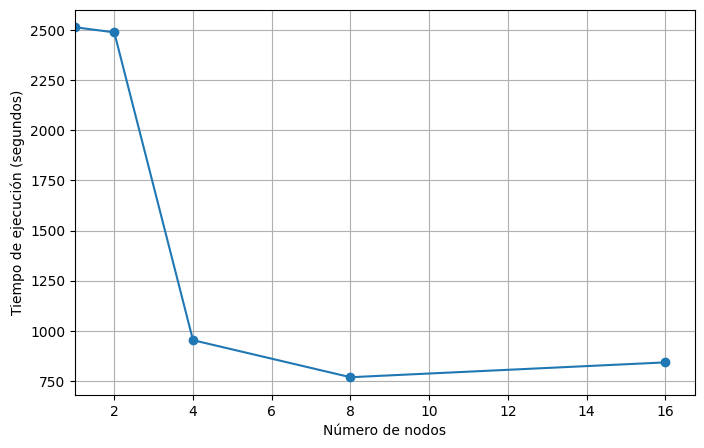
\includegraphics[width=0.8\textwidth]{imagenes/cap5/multi-node_ubuntu_cpu_native_time.png}
    \caption{Tiempo de ejecución en función del número de hebras en Ubuntu nativo (CPU) en entorno multiproceso.}
    \label{fig:multi-node_ubuntu_cpu_native_time}
\end{figure}

En la tabla \ref{tab:multi-node_ubuntu_cpu_native} se presentan los tiempos de ejecución y la variación porcentual respecto a una hebra.

\begin{table}[ht]
    \centering
    \begin{tabular}{|c|c|c|}
        \hline
        \textbf{Procesos} & \textbf{Tiempo de ejecución (s)} & \textbf{$\Delta$\% vs 1 proceso} \\
        \hline
        1                 & 2515.21                          & 0.00                             \\
        2                 & 2489.49                          & -1.02                            \\
        4                 & 952.85                           & -62.12                           \\
        8                 & 767.87                           & -69.47                           \\
        16                & 841.96                           & -66.53                           \\
        \hline
    \end{tabular}
    \caption{Tiempos de ejecución y variación porcentual respecto a un proceso en entorno multiproceso Ubuntu nativo (CPU).}
    \label{tab:multi-node_ubuntu_cpu_native}
\end{table}

La tabla muestra cómo varía el tiempo de ejecución al aumentar el número de procesos en un entorno multiproceso Ubuntu nativo usando CPU. Se observa que:

Al pasar de 1 a 2 procesos, la variación del tiempo es mínima (-1.02\%), lo que indica poca mejora.
Con 4 procesos, el tiempo baja significativamente (-62.12\%), mostrando una mejora notable en la paralelización.
Con 8 procesos, la reducción es aún mayor (69.47\%), aunque el beneficio adicional respecto a 4 procesos es menor.
Al aumentar a 16 procesos, el tiempo de ejecución aumenta ligeramente respecto a 8 procesos y la reducción porcentual disminuye (66.53\%), lo que sugiere que a partir de cierto punto añadir más procesos no mejora el rendimiento e incluso puede empeorarlo, posiblemente por sobrecarga de comunicación o gestión.

En resumen, la eficiencia de la paralelización mejora hasta cierto número de procesos, pero después se observa un efecto de saturación o incluso degradación del rendimiento.

En la figura \ref{fig:multi-node_ubuntu_cpu_native_cpu} se muestra el porcentaje de uso de CPU y la eficiencia en función del número de procesos en un entorno multiproceso con Ubuntu nativo.

\begin{figure}[ht]
    \centering
    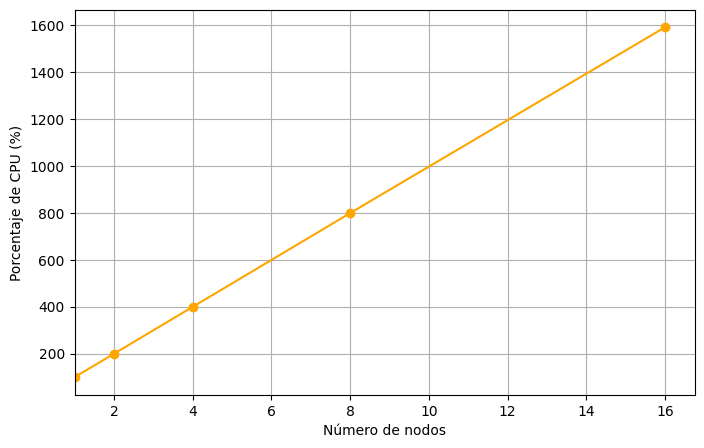
\includegraphics[width=0.8\textwidth]{imagenes/cap5/multi-node_ubuntu_cpu_native_cpu_time.png}
    \caption{Porcentaje de uso de CPU y eficiencia en función del número de procesos en Ubuntu nativo (CPU) en entorno multiproceso.}
    \label{fig:multi-node_ubuntu_cpu_native_cpu}
\end{figure}

En la tabla \ref{tab:multi-node_ubuntu_cpu_native_cpu} se presentan los porcentajes de uso de CPU y la eficiencia correspondiente.

\begin{table}[ht]
    \centering
    \small
    \setlength{\tabcolsep}{4pt}
    \renewcommand{\arraystretch}{1.1}
    \begin{tabular}{|c|c|c|c|}
        \hline
        \textbf{Procesos} & \textbf{Porcentaje de CPU (\%)} & \textbf{Max uso CPU (\%)} & \textbf{Eficiencia CPU (\%)} \\
        \hline
        1                 & 99.00                           & 100.00                    & 99.00                        \\
        2                 & 199.00                          & 200.00                    & 99.50                        \\
        4                 & 399.00                          & 400.00                    & 99.75                        \\
        8                 & 799.00                          & 800.00                    & 99.88                        \\
        16                & 1592.00                         & 1600.00                   & 99.50                        \\
        \hline
    \end{tabular}
    \caption{Porcentaje de uso de CPU y eficiencia en función del número de procesos en Ubuntu nativo (CPU) en entorno multiproceso.}
    \label{tab:multi-node_ubuntu_cpu_native_cpu}
\end{table}

La tabla muestra el porcentaje de uso de CPU y la eficiencia al aumentar el número de procesos en un entorno multiproceso Ubuntu nativo (CPU):

El uso de CPU escala casi linealmente con el número de procesos, lo que indica que los recursos se están utilizando de manera efectiva. El valor "Max uso CPU" representa el uso máximo teórico (número de procesos $\times$ 100\%), y el uso real está muy cerca de ese máximo en todos los casos. La eficiencia de CPU se mantiene muy alta (entre 99.00\% y 99.88\%) para todos los escenarios, lo que sugiere que la sobrecarga de paralelización es mínima y que el sistema aprovecha casi todo el potencial de los recursos disponibles. Solo con 16 procesos se observa una ligera caída en la eficiencia (99.50\%), pero sigue siendo excelente.

En resumen, el sistema mantiene una eficiencia de CPU muy alta al escalar el número de procesos, lo que indica una buena gestión de los recursos y una paralelización efectiva en este entorno.

\subsubsection{CPU + GPU}

La figura \ref{fig:multi-node_ubuntu_gpu_native_time} muestra el tiempo de ejecución para la configuración de CPU + GPU en un entorno multiproceso con Ubuntu nativo.

\begin{figure}[ht]
    \centering
    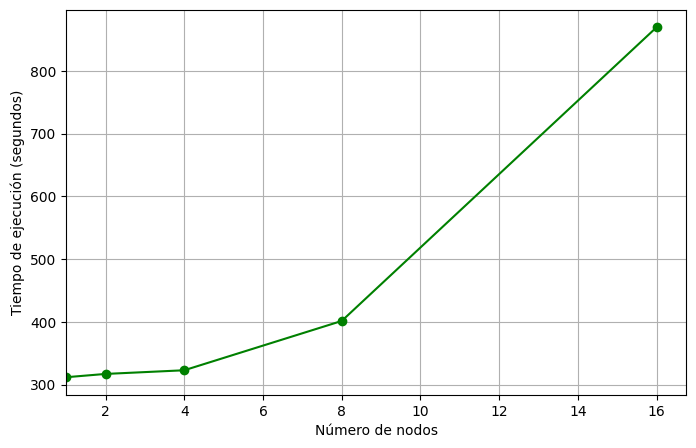
\includegraphics[width=0.8\textwidth]{imagenes/cap5/multi-node_ubuntu_gpu_native_time.png}
    \caption{Tiempo de ejecución en función del número de hebras en Ubuntu nativo (CPU + GPU) en entorno multiproceso.}
    \label{fig:multi-node_ubuntu_gpu_native_time}
\end{figure}

En la tabla \ref{tab:multi-node_ubuntu_gpu_native} se presentan los tiempos de ejecución y la variación porcentual respecto a una hebra.

\begin{table}[ht]
    \centering
    \begin{tabular}{|c|c|c|}
        \hline
        \textbf{Procesos} & \textbf{Tiempo (s)} & \textbf{$\Delta$\% vs 1 proceso} \\
        \hline
        1                 & 311.68              & 0.00                             \\
        2                 & 316.92              & 1.68                             \\
        4                 & 322.77              & 3.56                             \\
        8                 & 401.33              & 28.76                            \\
        16                & 869.40              & 178.94                           \\
        \hline
    \end{tabular}
    \caption{Tiempos de ejecución y variación porcentual respecto a un proceso en entorno multiproceso Ubuntu nativo (CPU + GPU).}
    \label{tab:multi-node_ubuntu_gpu_native}
\end{table}

La tabla muestra los tiempos de ejecución y la variación porcentual al aumentar el número de procesos en un entorno multiproceso Ubuntu nativo utilizando CPU y GPU:

Con un solo proceso, el tiempo base es de 311.68\,s. Al incrementar a 2 y 4 procesos, el tiempo de ejecución aumenta ligeramente (316.92\,s y 322.77\,s), lo que implica una pequeña penalización en lugar de una mejora (variaciones positivas del 1.68\% y 3.56\%). Con 8 procesos, el tiempo sube notablemente hasta 401.33\,s (+28.76\%), y con 16 procesos el incremento es aún mayor (869.40\,s, +178.94\%).

Estos resultados indican que, a diferencia del caso solo CPU, al añadir más procesos con GPU el rendimiento empeora progresivamente. Es probable que la sobrecarga de comunicación, la gestión de recursos compartidos o la falta de escalabilidad de la aplicación para GPU estén afectando negativamente. En este entorno, la paralelización no solo no aporta beneficios, sino que resulta contraproducente a partir de más de un proceso.

\subsubsection{Comparativa CPU vs CPU + GPU}

En la figura \ref{fig:multi-node_ubuntu_cpu_vs_gpu_native_time} se muestra una comparativa del tiempo de ejecución entre las configuraciones CPU y CPU + GPU en un entorno multiproceso con Ubuntu nativo.

\begin{figure}[ht]
    \centering
    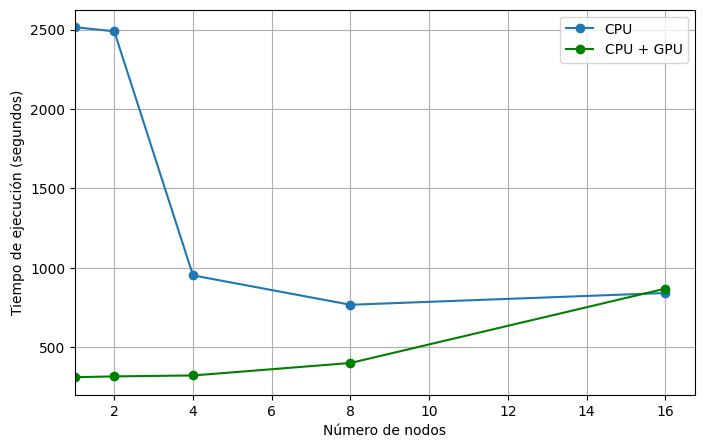
\includegraphics[width=0.8\textwidth]{imagenes/cap5/multi-node_ubuntu_cpu_vs_gpu_native_time.png}
    \caption{Comparativa de tiempo de ejecución entre CPU y CPU + GPU en función del número de procesos en Ubuntu nativo en entorno multiproceso.}
    \label{fig:multi-node_ubuntu_cpu_vs_gpu_native_time}
\end{figure}

En la tabla \ref{tab:multi-node_ubuntu_cpu_vs_gpu_native} se presentan los tiempos de ejecución para ambas configuraciones y la variación porcentual entre ellas.

\begin{table}[ht]
    \centering
    \begin{tabular}{|c|c|c|c|}
        \hline
        \textbf{Procesos} & \textbf{Tiempo CPU (s)} & \textbf{Tiempo CPU+GPU (s)} & \textbf{Variación (\%)} \\
        \hline
        1                 & 2515.21                 & 311.68                      & -87.61                  \\
        2                 & 2489.49                 & 316.92                      & -87.27                  \\
        4                 & 952.85                  & 322.77                      & -66.13                  \\
        8                 & 767.87                  & 401.33                      & -47.73                  \\
        16                & 841.96                  & 869.40                      & 3.26                    \\
        \hline
    \end{tabular}
    \caption{Comparativa de tiempos de ejecución entre CPU y CPU+GPU en función del número de procesos en Ubuntu nativo (multiproceso) y variación porcentual.}
    \label{tab:multi-node_ubuntu_cpu_vs_gpu_native}
\end{table}

La tabla muestra que, con uno y dos procesos, la configuración CPU+GPU es considerablemente más rápida que la opción solo CPU, con reducciones de tiempo superiores al 87\%. Esto evidencia un beneficio claro del uso de GPU en escenarios con pocos procesos. Al aumentar a cuatro y ocho procesos, la ventaja de la GPU disminuye: la reducción es del 66.13\% con cuatro procesos y del 47.73\% con ocho procesos. Aunque la GPU sigue proporcionando mejores tiempos, la diferencia se reduce conforme se incrementa el número de procesos. Con dieciséis procesos, la situación se invierte y el tiempo de CPU+GPU resulta ligeramente superior al de solo CPU, con una variación positiva del 3.26\%. Esto sugiere que, a partir de cierto punto, la sobrecarga asociada al uso de GPU y la comunicación entre procesos supera los beneficios de la aceleración.

En resumen, el uso de GPU aporta grandes mejoras en los tiempos de ejecución para un bajo número de procesos, pero su escalabilidad es limitada. A medida que se incrementa el número de procesos, la eficiencia de la GPU disminuye y puede llegar a ser contraproducente, probablemente debido a la sobrecarga de comunicación y la gestión de recursos en entornos multiproceso.

\subsection{Ejecución en contenedores de Ubuntu}
\subsubsection{CPU}

En la figura \ref{fig:multi-node_ubuntu_docker_time} se muestra el tiempo de ejecución para la configuración de CPU en un entorno multiproceso con contenedores de Ubuntu.

\begin{figure}[ht]
    \centering
    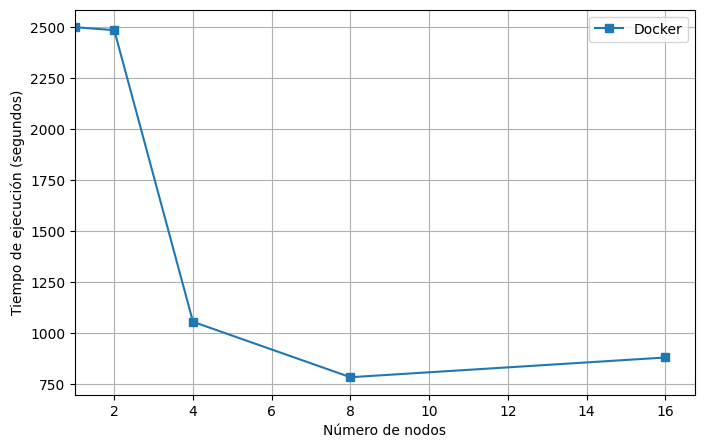
\includegraphics[width=0.8\textwidth]{imagenes/cap5/multi-node_ubuntu_docker_time.png}
    \caption{Tiempo de ejecución en función del número de hebras en contenedores de Ubuntu (CPU) en entorno multiproceso.}
    \label{fig:multi-node_ubuntu_docker_time}
\end{figure}

En la tabla \ref{tab:multi-node_ubuntu_docker} se presentan los tiempos de ejecución y la variación porcentual respecto a una hebra.

\begin{table}[ht]
    \centering
    \begin{tabular}{|c|c|c|}
        \hline
        \textbf{Procesos} & \textbf{Tiempo (s)} & \textbf{$\Delta$\% vs 1 proceso} \\
        \hline
        1                 & 2499.09             & 0.00                             \\
        2                 & 2484.80             & -0.57                            \\
        4                 & 1054.20             & -57.82                           \\
        8                 & 782.42              & -68.69                           \\
        16                & 879.20              & -64.82                           \\
        \hline
    \end{tabular}
    \caption{Tiempos de ejecución y variación porcentual respecto a un proceso en entorno multiproceso con contenedores de Ubuntu (CPU).}
    \label{tab:multi-node_ubuntu_docker}
\end{table}

De 1 a 2 procesos, la mejora es mínima (-0.57\%), lo que indica que la paralelización apenas aporta beneficio en este rango. Con 4 procesos, la reducción es significativa (57.82\%), mostrando una mejora clara en el rendimiento gracias a la paralelización. Con 8 procesos, la reducción alcanza el 68.69\%, lo que indica un buen aprovechamiento de los recursos al escalar. Con 16 procesos, el tiempo de ejecución aumenta ligeramente respecto a 8 procesos y la reducción porcentual disminuye a -64.82\%, lo que sugiere que a partir de cierto punto la eficiencia se ve limitada, posiblemente por la sobrecarga de coordinación y comunicación entre contenedores.

En resumen, el entorno con contenedores de Ubuntu permite una buena escalabilidad hasta 8 procesos, con mejoras notables en el tiempo de ejecución. Sin embargo, al aumentar a 16 procesos, la eficiencia disminuye, mostrando un comportamiento similar al entorno nativo: la paralelización es efectiva hasta cierto límite, tras el cual la sobrecarga afecta negativamente al rendimiento.

En la figura \ref{fig:multi-node_ubuntu_podman} se muestra el tiempo de ejecución para la configuración de CPU en un entorno multiproceso con contenedores de \textit{Podman}.

\begin{figure}[ht]
    \centering
    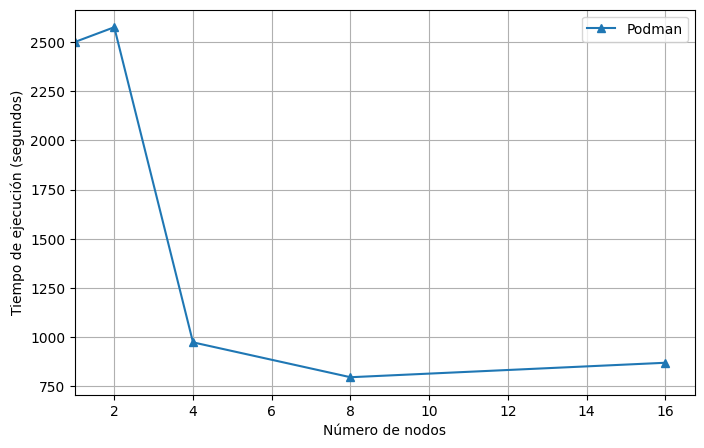
\includegraphics[width=0.8\textwidth]{imagenes/cap5/multi-node_ubuntu_podman_time.png}
    \caption{Tiempo de ejecución en función del número de hebras en contenedores de \textit{Podman} (CPU) en entorno multiproceso.}
    \label{fig:multi-node_ubuntu_podman}
\end{figure}

En la tabla \ref{tab:multi-node_ubuntu_podman} se presentan los tiempos de ejecución y la reducción porcentual respecto a una hebra.

\begin{table}[ht]
    \centering
    \begin{tabular}{|c|c|c|}
        \hline
        \textbf{Procesos} & \textbf{Tiempo (s)} & \textbf{$\Delta$\% vs 1 proceso} \\
        \hline
        1                 & 2499.16             & 0.00                             \\
        2                 & 2574.04             & 3.00                             \\
        4                 & 973.92              & -61.03                           \\
        8                 & 796.84              & -68.12                           \\
        16                & 870.28              & -65.18                           \\
        \hline
    \end{tabular}
    \caption{Tiempos de ejecución y reducción porcentual respecto a un proceso en entorno multiproceso con contenedores de \textit{Podman} (CPU).}
    \label{tab:multi-node_ubuntu_podman}
\end{table}

La tabla muestra cómo varía el tiempo de ejecución al aumentar el número de procesos en un entorno multiproceso utilizando contenedores de \textit{Podman} sobre CPU. Con un solo proceso se establece el tiempo base, mientras que al duplicar el número de procesos a dos, se observa un ligero aumento en el tiempo de ejecución, lo que indica que la paralelización no solo no aporta mejoras en este caso, sino que introduce una pequeña penalización, probablemente debida a la sobrecarga de gestión de los contenedores. Sin embargo, al incrementar a cuatro procesos, el tiempo de ejecución disminuye considerablemente, reflejando una reducción del 61.03\% respecto al caso de un proceso, lo que evidencia una mejora significativa en el rendimiento gracias a la paralelización. Esta tendencia positiva se mantiene con ocho procesos, donde la reducción alcanza el 68.12\%, mostrando un buen aprovechamiento de los recursos disponibles. No obstante, al aumentar a dieciséis procesos, el tiempo de ejecución vuelve a incrementarse ligeramente y la reducción porcentual disminuye a 65.18\%, lo que sugiere que, a partir de cierto punto, la eficiencia de la paralelización se ve limitada, posiblemente por la sobrecarga de coordinación y comunicación entre los contenedores. En conjunto, el entorno con \textit{Podman} permite una escalabilidad efectiva hasta un número intermedio de procesos, pero muestra limitaciones cuando se incrementa excesivamente el grado de paralelismo.

\subsubsection{CPU + GPU}

En la figura \ref{fig:multi-node_ubuntu_docker_gpu_time} se muestra el tiempo de ejecución para la configuración de CPU + GPU en un entorno multiproceso con contenedores de Ubuntu.

\begin{figure}[ht]
    \centering
    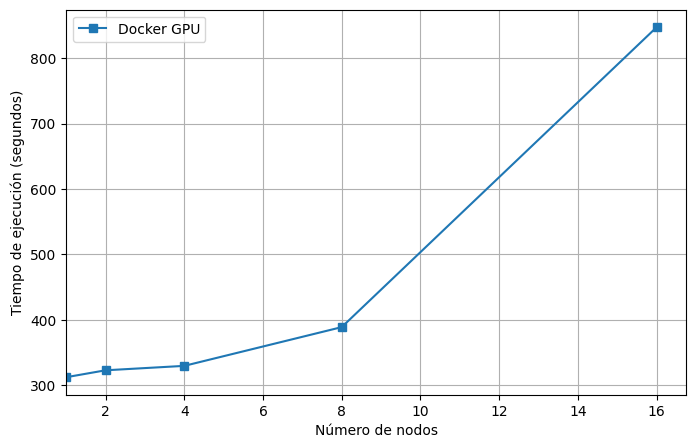
\includegraphics[width=0.8\textwidth]{imagenes/cap5/multi-node_ubuntu_docker_gpu_time.png}
    \caption{Tiempo de ejecución en función del número de hebras en contenedores de Ubuntu (CPU + GPU) en entorno multiproceso.}
    \label{fig:multi-node_ubuntu_docker_gpu_time}
\end{figure}

En la tabla \ref{tab:multi-node_ubuntu_docker_gpu} se presentan los tiempos de ejecución y la reducción porcentual respecto a una hebra.

\begin{table}[ht]
    \centering
    \begin{tabular}{|c|c|c|}
        \hline
        \textbf{Procesos} & \textbf{Tiempo (s)} & \textbf{$\Delta$\% vs 1 proceso} \\
        \hline
        1                 & 312.18              & 0.00                             \\
        2                 & 322.77              & 3.39                             \\
        4                 & 329.54              & 5.56                             \\
        8                 & 388.78              & 24.54                            \\
        16                & 847.37              & 171.44                           \\
        \hline
    \end{tabular}
    \caption{Tiempos de ejecución y variación porcentual respecto a un proceso en entorno multiproceso con contenedores de Ubuntu (CPU + GPU).}
    \label{tab:multi-node_ubuntu_docker_gpu}
\end{table}

La tabla refleja el comportamiento del tiempo de ejecución al aumentar el número de procesos en un entorno multiproceso con contenedores de Ubuntu utilizando tanto CPU como GPU. Con un solo proceso, el tiempo de ejecución es el más bajo, sirviendo como referencia para el resto de configuraciones. Al incrementar a dos y cuatro procesos, lejos de mejorar, el tiempo de ejecución aumenta ligeramente, lo que se traduce en una variación porcentual positiva y evidencia que la paralelización en este contexto no resulta beneficiosa, probablemente debido a la sobrecarga de coordinación y a la gestión de recursos entre los contenedores y las GPUs. Esta tendencia se acentúa al llegar a ocho procesos, donde el tiempo de ejecución sigue incrementándose y la penalización alcanza el 24.54\%. Finalmente, con dieciséis procesos, el tiempo de ejecución se eleva de forma considerable, con una variación porcentual del 171.44\% respecto al caso de un solo proceso. Estos resultados indican que, en este entorno, la escalabilidad es muy limitada y que el uso combinado de contenedores y GPU no solo no aporta mejoras al aumentar el número de procesos, sino que puede llegar a ser claramente contraproducente, probablemente por la complejidad añadida en la gestión de los recursos y la comunicación entre procesos.

En la figura \ref{fig:multi-node_ubuntu_podman_gpu_time} se muestra el tiempo de ejecución para la configuración de CPU + GPU en un entorno multiproceso con contenedores de \textit{Podman}.

\begin{figure}[ht]
    \centering
    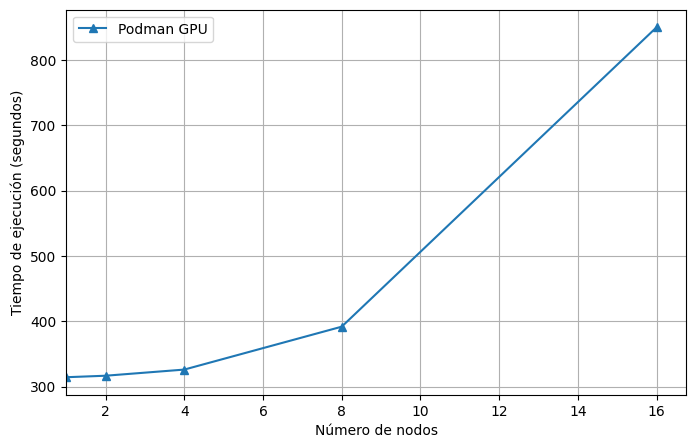
\includegraphics[width=0.8\textwidth]{imagenes/cap5/multi-node_ubuntu_podman_gpu_time.png}
    \caption{Tiempo de ejecución en función del número de hebras en contenedores de \textit{Podman} (CPU + GPU) en entorno multiproceso.}
    \label{fig:multi-node_ubuntu_podman_gpu_time}
\end{figure}

En la tabla \ref{tab:multi-node_ubuntu_podman_gpu} se presentan los tiempos de ejecución y la reducción porcentual respecto a una hebra.

\begin{table}[ht]
    \centering
    \begin{tabular}{|c|c|c|}
        \hline
        \textbf{Procesos} & \textbf{Tiempo (s)} & \textbf{$\Delta$\% vs 1 proceso} \\
        \hline
        1                 & 314.51              & 0.00                             \\
        2                 & 316.80              & 0.73                             \\
        4                 & 326.20              & 3.72                             \\
        8                 & 391.86              & 24.59                            \\
        16                & 850.18              & 170.32                           \\
        \hline
    \end{tabular}
    \caption{Tiempos de ejecución y variación porcentual respecto a un proceso en entorno multiproceso con contenedores de \textit{Podman} (CPU + GPU).}
    \label{tab:multi-node_ubuntu_podman_gpu}
\end{table}

La tabla muestra la evolución del tiempo de ejecución al aumentar el número de procesos en un entorno multiproceso con contenedores de \textit{Podman} utilizando tanto CPU como GPU. Con un solo proceso, el tiempo de ejecución es el más bajo y sirve como referencia. Al pasar a dos y cuatro procesos, se observa un ligero incremento en el tiempo de ejecución, con variaciones porcentuales positivas que indican que la paralelización no aporta mejoras y, de hecho, introduce una pequeña penalización, probablemente debida a la sobrecarga de coordinación y gestión de recursos entre los contenedores y las GPUs. Esta tendencia se intensifica al aumentar a ocho procesos, donde el tiempo de ejecución crece de manera más notable y la penalización alcanza el 24.59\%. Finalmente, con dieciséis procesos, el tiempo de ejecución se incrementa considerablemente, con una variación porcentual del 170.32\% respecto al caso de un solo proceso. Estos resultados evidencian que, en este entorno, la escalabilidad es muy limitada y que el uso combinado de contenedores \textit{Podman} y GPU no solo no mejora el rendimiento al aumentar el número de procesos, sino que puede resultar claramente perjudicial, probablemente debido a la complejidad añadida en la gestión de recursos y la comunicación entre procesos.

\subsubsection{Comparativa contenedores vs nativo}

En la figura \ref{fig:multi-node_ubuntu_container_vs_native_time} se muestra una comparativa del tiempo de ejecución entre las configuraciones nativo y contenedores de Ubuntu en un entorno multiproceso con CPU.

\begin{figure}[ht]
    \centering
    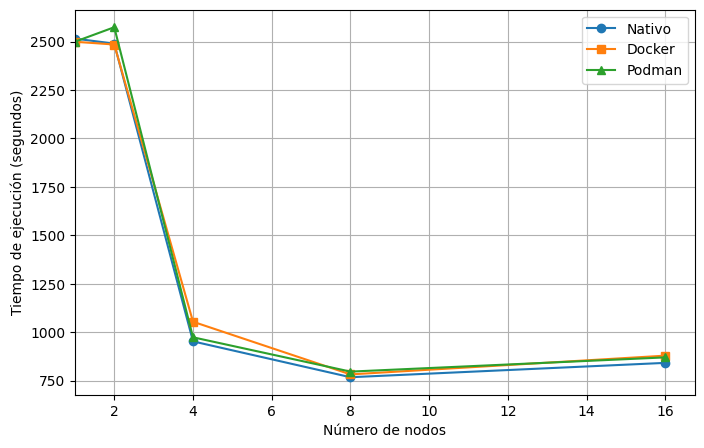
\includegraphics[width=0.8\textwidth]{imagenes/cap5/multi-node_ubuntu_container_vs_native_time.png}
    \caption{Comparativa de tiempo de ejecución entre nativo y contenedores de Ubuntu en función del número de procesos en entorno multiproceso (CPU).}
    \label{fig:multi-node_ubuntu_container_vs_native_time}
\end{figure}

En la tabla \ref{tab:multi-node_ubuntu_container_vs_native} se presentan los tiempos de ejecución para ambas configuraciones y la variación porcentual entre ellas.

\begin{table}[ht]
    \centering
    \small
    \setlength{\tabcolsep}{4pt}
    \renewcommand{\arraystretch}{1.1}
    \begin{tabular}{|c|c|c|c|c|c|}
        \hline
        \textbf{Procesos} & \textbf{Nativo (s)} & \textbf{\textit{Docker} (s)} & \textbf{\textit{Docker} $\Delta$\%} & \textbf{\textit{Podman} (s)} & \textbf{\textit{Podman} $\Delta$\%} \\
        \hline
        1                 & 2515.21             & 2499.09                      & -0.64                               & 2499.16                      & -0.64                               \\
        2                 & 2489.49             & 2484.80                      & -0.19                               & 2574.04                      & 3.40                                \\
        4                 & 952.85              & 1054.20                      & 10.64                               & 973.92                       & 2.21                                \\
        8                 & 767.87              & 782.42                       & 1.89                                & 796.84                       & 3.77                                \\
        16                & 841.96              & 879.20                       & 4.42                                & 870.28                       & 3.36                                \\
        \hline
    \end{tabular}
    \caption{Comparativa de tiempos de ejecución entre nativo, \textit{Docker} y \textit{Podman} en función del número de procesos en entorno multiproceso (CPU) y variación porcentual respecto a nativo.}
    \label{tab:multi-node_ubuntu_container_vs_native}
\end{table}

La tabla presenta una comparación de los tiempos de ejecución entre los entornos nativo, \textit{Docker} y \textit{Podman} en un escenario multiproceso utilizando únicamente CPU, así como la variación porcentual de los contenedores respecto al entorno nativo. Con un solo proceso, tanto \textit{Docker} como \textit{Podman} muestran tiempos de ejecución ligeramente inferiores al nativo, con una reducción del 0.64\%, lo que indica que la sobrecarga de los contenedores es prácticamente inexistente en este caso. Al aumentar a dos procesos, \textit{Docker} mantiene una ligera mejora, mientras que \textit{Podman} experimenta un incremento del 3.40\% en el tiempo de ejecución, sugiriendo que la eficiencia de los contenedores puede variar según la tecnología empleada y la carga de trabajo. Con cuatro procesos, \textit{Docker} presenta un aumento notable del 10.64\% respecto al nativo, mientras que \textit{Podman} solo incrementa un 2.21\%, lo que podría estar relacionado con la gestión interna de los recursos y la coordinación entre contenedores. A medida que se incrementa el número de procesos a ocho y dieciséis, tanto \textit{Docker} como \textit{Podman} muestran incrementos moderados en los tiempos de ejecución respecto al entorno nativo, aunque las diferencias se mantienen en valores relativamente bajos. En conjunto, los resultados indican que el uso de contenedores en entornos multiproceso con CPU introduce una sobrecarga mínima o moderada en la mayoría de los casos, siendo \textit{Docker} algo más sensible a la escalabilidad en configuraciones intermedias. Sin embargo, la viabilidad de los contenedores para la ejecución de aplicaciones paralelas y distribuidas se mantiene, ya que las diferencias de rendimiento respecto al entorno nativo no son excesivamente significativas.

En la figura \ref{fig:multi-node_ubuntu_container_vs_native_gpu_time} se muestra una comparativa del tiempo de ejecución entre las configuraciones nativo y contenedores de Ubuntu en un entorno multiproceso con CPU + GPU.

\begin{figure}[ht]
    \centering
    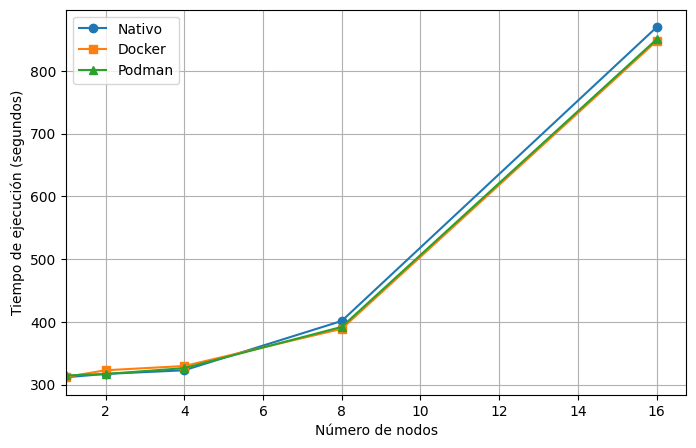
\includegraphics[width=0.8\textwidth]{imagenes/cap5/multi-node_ubuntu_container_vs_native_gpu_time.png}
    \caption{Comparativa de tiempo de ejecución entre nativo y contenedores de Ubuntu en función del número de procesos en entorno multiproceso (CPU + GPU).}
    \label{fig:multi-node_ubuntu_container_vs_native_gpu_time}
\end{figure}

En la tabla \ref{tab:multi-node_ubuntu_container_vs_native_gpu} se presentan los tiempos de ejecución para ambas configuraciones y la variación porcentual entre ellas.

\begin{table}[ht]
    \centering
    \small
    \setlength{\tabcolsep}{4pt}
    \renewcommand{\arraystretch}{1.1}
    \begin{tabular}{|c|c|c|c|c|c|}
        \hline
        \textbf{Procesos} & \textbf{Nativo (s)} & \textbf{\textit{Docker} (s)} & \textbf{\textit{Docker} $\Delta$\%} & \textbf{\textit{Podman} (s)} & \textbf{\textit{Podman} $\Delta$\%} \\
        \hline
        1                 & 311.68              & 312.18                       & 0.16                                & 314.51                       & 0.91                                \\
        2                 & 316.92              & 322.77                       & 1.85                                & 316.80                       & -0.04                               \\
        4                 & 322.77              & 329.54                       & 2.10                                & 326.20                       & 1.06                                \\
        8                 & 401.33              & 388.78                       & -3.13                               & 391.86                       & -2.36                               \\
        16                & 869.40              & 847.37                       & -2.53                               & 850.18                       & -2.21                               \\
        \hline
    \end{tabular}
    \caption{Comparativa de tiempos de ejecución entre nativo, \textit{Docker} y \textit{Podman} en función del número de procesos en entorno multiproceso (CPU+GPU) y variación porcentual respecto a nativo.}
    \label{tab:multi-node_ubuntu_container_vs_native_gpu}
\end{table}

La tabla compara los tiempos de ejecución en un entorno multiproceso con CPU y GPU para las configuraciones nativa, \textit{Docker} y \textit{Podman}, mostrando también la variación porcentual de los contenedores respecto al entorno nativo. Con un solo proceso, tanto \textit{Docker} como \textit{Podman} presentan tiempos de ejecución prácticamente idénticos al entorno nativo, con diferencias inferiores al 1\%, lo que indica que la sobrecarga de los contenedores es despreciable en este escenario. Al aumentar a dos y cuatro procesos, \textit{Docker} muestra un ligero incremento en el tiempo de ejecución respecto al nativo, mientras que \textit{Podman} se mantiene prácticamente igual o con una diferencia muy pequeña, lo que sugiere que ambos sistemas de contenedores gestionan eficientemente la paralelización en estos casos. Sin embargo, al escalar a ocho y dieciséis procesos, tanto \textit{Docker} como \textit{Podman} presentan tiempos de ejecución ligeramente inferiores a los del entorno nativo, con variaciones negativas que indican una mejora marginal en el rendimiento. Este comportamiento puede deberse a pequeñas diferencias en la gestión de recursos o a la forma en que los contenedores distribuyen la carga de trabajo. En conjunto, los resultados muestran que el uso de contenedores, tanto \textit{Docker} como \textit{Podman}, no introduce penalizaciones significativas en el rendimiento respecto al entorno nativo y, en algunos casos, incluso puede aportar ligeras mejoras al aumentar el número de procesos, lo que demuestra la viabilidad de estas tecnologías para la ejecución de aplicaciones paralelas y distribuidas en entornos multiproceso con aceleración por GPU.

\subsection{Ejecución en contenedores de Windows}
\subsubsection{CPU}

En la figura \ref{fig:multi-node_windows_docker_time} se muestra el tiempo de ejecución para la configuración de CPU en un entorno multiproceso con contenedores de Windows.

\begin{figure}[ht]
    \centering
    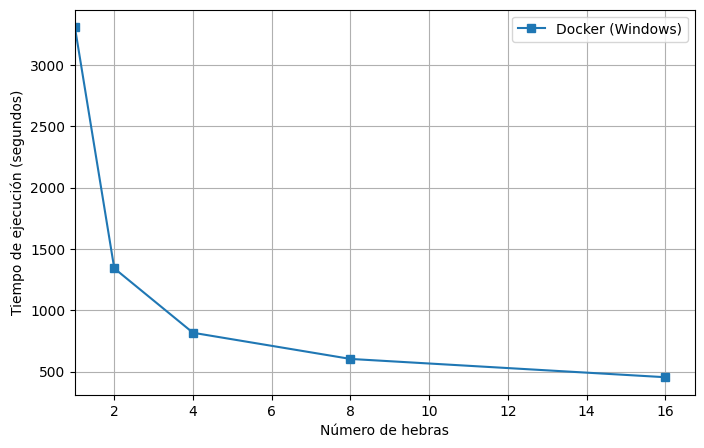
\includegraphics[width=0.8\textwidth]{imagenes/cap5/multi-node_windows_docker_time.png}
    \caption{Tiempo de ejecución en función del número de hebras en contenedores de Windows (CPU) en entorno multiproceso.}
    \label{fig:multi-node_windows_docker_time}
\end{figure}

En la tabla \ref{tab:multi-node_windows_docker} se presentan los tiempos de ejecución y la reducción porcentual respecto a una hebra.

\begin{table}[ht]
    \centering
    \begin{tabular}{|c|c|c|}
        \hline
        \textbf{Procesos} & \textbf{Tiempo (s)} & \textbf{$\Delta$\% vs 1 proceso} \\
        \hline
        1                 & 3308.08             & 0.00                             \\
        2                 & 2708.91             & -18.11                           \\
        4                 & 1185.46             & -64.16                           \\
        8                 & 1090.62             & -67.03                           \\
        16                & 930.79              & -71.86                           \\
        \hline
    \end{tabular}
    \caption{Tiempos de ejecución y reducción porcentual respecto a un proceso en entorno multiproceso con contenedores de Windows (CPU).}
    \label{tab:multi-node_windows_docker}
\end{table}

La tabla muestra la evolución del tiempo de ejecución al aumentar el número de procesos en un entorno multiproceso con contenedores de Windows utilizando CPU. Con un solo proceso, el tiempo de ejecución es el más alto y sirve como referencia para el resto de configuraciones. Al duplicar el número de procesos a dos, se observa una reducción significativa del 18.11\% en el tiempo de ejecución, lo que indica que la paralelización comienza a aportar beneficios claros. Esta mejora se acentúa al incrementar a cuatro procesos, donde la reducción alcanza el 64.16\%, reflejando una eficiencia notable en la distribución de la carga de trabajo. Con ocho procesos, la reducción porcentual es del 67.03\%, lo que demuestra que el sistema sigue escalando de manera eficiente. Finalmente, al llegar a dieciséis procesos, el tiempo de ejecución disminuye aún más, con una reducción del 71.86\% respecto al caso de un solo proceso. Estos resultados evidencian que el entorno multiproceso con contenedores de Windows permite una escalabilidad efectiva y un aprovechamiento eficiente de los recursos al aumentar el número de procesos, logrando mejoras sustanciales en el rendimiento conforme se incrementa el grado de paralelismo.

En la figura \ref{fig:multi-node_windows_podman_time} se muestra el tiempo de ejecución para la configuración de CPU en un entorno multiproceso con contenedores de \textit{Podman} en Windows.

\begin{figure}[ht]
    \centering
    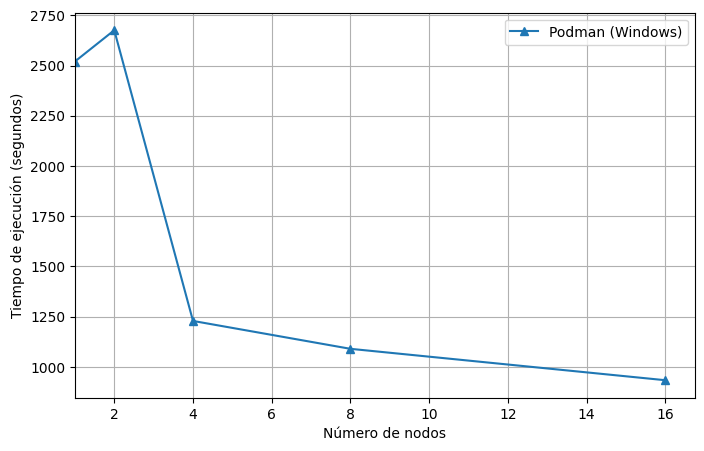
\includegraphics[width=0.8\textwidth]{imagenes/cap5/multi-node_windows_podman_time.png}
    \caption{Tiempo de ejecución en función del número de hebras en contenedores de \textit{Podman} (CPU) en entorno multiproceso.}
    \label{fig:multi-node_windows_podman_time}
\end{figure}

En la tabla \ref{tab:multi-node_windows_podman} se presentan los tiempos de ejecución y la reducción porcentual respecto a una hebra.

\begin{table}[ht]
    \centering
    \begin{tabular}{|c|c|c|}
        \hline
        \textbf{Procesos} & \textbf{Tiempo (s)} & \textbf{$\Delta$\% vs 1 proceso} \\
        \hline
        1.00              & 2520.21             & 0.00                             \\
        2.00              & 2675.94             & 6.18                             \\
        4.00              & 1228.59             & -51.25                           \\
        8.00              & 1089.75             & -56.76                           \\
        16.00             & 933.45              & -62.96                           \\
        \hline
    \end{tabular}
    \caption{Tiempos de ejecución y reducción porcentual respecto a un proceso en entorno multiproceso con contenedores de \textit{Podman} en Windows (CPU).}
    \label{tab:multi-node_windows_podman}
\end{table}

La tabla presenta la evolución del tiempo de ejecución al aumentar el número de procesos en un entorno multiproceso con contenedores de \textit{Podman} sobre Windows utilizando CPU. Con un solo proceso, se establece el tiempo de referencia. Al pasar a dos procesos, se observa un incremento del 6.18\% en el tiempo de ejecución, lo que indica que la paralelización en este caso introduce una penalización inicial, probablemente debida a la sobrecarga de coordinación o a la gestión de recursos en el entorno de contenedores sobre Windows. Sin embargo, al aumentar a cuatro procesos, el tiempo de ejecución disminuye de forma considerable, con una reducción del 51.25\%, lo que evidencia una mejora significativa en el rendimiento gracias a la paralelización. Esta tendencia positiva se mantiene al escalar a ocho y dieciséis procesos, donde las reducciones alcanzan el 56.76\% y el 62.96\% respectivamente, mostrando que el sistema es capaz de aprovechar de manera eficiente los recursos adicionales a medida que se incrementa el número de procesos. En conjunto, los resultados indican que, aunque existe una penalización inicial al duplicar los procesos, el entorno multiproceso con contenedores de \textit{Podman} en Windows logra una escalabilidad efectiva y una mejora sustancial del rendimiento a partir de cuatro procesos, confirmando la viabilidad de esta tecnología para la ejecución de aplicaciones paralelas en este contexto.

\subsubsection{CPU + GPU}

En la figura \ref{fig:multi-node_windows_docker_gpu_time} se muestra el tiempo de ejecución para la configuración de CPU + GPU en un entorno multiproceso con contenedores de Ubuntu.

\begin{figure}[ht]
    \centering
    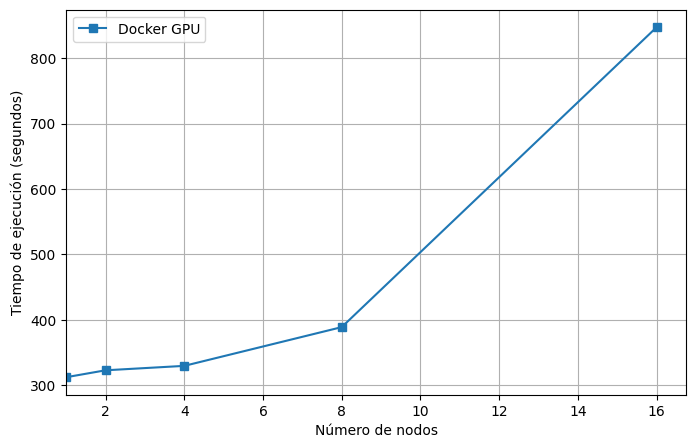
\includegraphics[width=0.8\textwidth]{imagenes/cap5/multi-node_ubuntu_docker_gpu_time.png}
    \caption{Tiempo de ejecución en función del número de hebras en contenedores de Windows (CPU + GPU) en entorno multiproceso.}
    \label{fig:multi-node_windows_docker_gpu_time}
\end{figure}

En la tabla \ref{tab:multi-node_windows_docker_gpu} se presentan los tiempos de ejecución y la reducción porcentual respecto a una hebra.

\begin{table}[ht]
    \centering
    \begin{tabular}{|c|c|c|}
        \hline
        \textbf{Procesos} & \textbf{Tiempo (s)} & \textbf{$\Delta$\% vs 1 proceso} \\
        \hline
        1                 & 312.18              & 0.00                             \\
        2                 & 322.77              & 3.39                             \\
        4                 & 329.54              & 5.56                             \\
        8                 & 388.78              & 24.54                            \\
        16                & 847.37              & 171.44                           \\
        \hline
    \end{tabular}
    \caption{Tiempos de ejecución y variación porcentual respecto a un proceso en entorno multiproceso con contenedores de Windows (CPU + GPU).}
    \label{tab:multi-node_windows_docker_gpu}
\end{table}

Al incrementar el número de procesos, lejos de reducirse, el tiempo de ejecución aumenta de forma progresiva, alcanzando un 171.44\% más con 16 procesos en comparación con la ejecución monoproceso.

Incluso con 2 o 4 procesos, el tiempo de ejecución resulta ligeramente superior al obtenido con un solo proceso, lo que evidencia la ausencia de beneficios de paralelización en este entorno multiproceso.

Este aumento en el tiempo de ejecución indica la presencia de una sobrecarga considerable asociada tanto a la gestión de múltiples procesos como al acceso concurrente a la GPU, lo que deriva en un rendimiento inferior al esperado.

En consecuencia, estos resultados ponen de manifiesto que, en contenedores de Windows con CPU+GPU, la ejecución multiproceso no resulta eficiente e incluso puede ser contraproducente, siendo recomendable optar por la ejecución monoproceso para maximizar el rendimiento.

En la figura \ref{fig:multi-node_windows_podman_gpu_time} se muestra el tiempo de ejecución para la configuración de CPU + GPU en un entorno multiproceso con contenedores de \textit{Podman}.

\begin{figure}[ht]
    \centering
    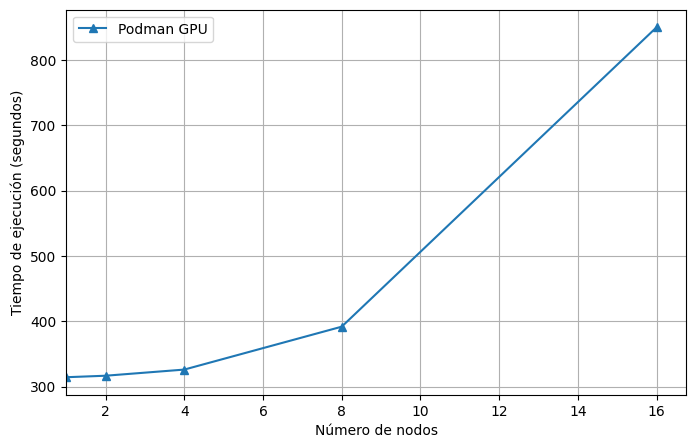
\includegraphics[width=0.8\textwidth]{imagenes/cap5/multi-node_ubuntu_podman_gpu_time.png}
    \caption{Tiempo de ejecución en función del número de hebras en contenedores de \textit{Podman} (CPU + GPU) en entorno multiproceso.}
    \label{fig:multi-node_ubuntu_podman_gpu_time}
\end{figure}

En la tabla \ref{tab:multi-node_windows_podman_gpu} se presentan los tiempos de ejecución y la reducción porcentual respecto a una hebra.

\begin{table}[ht]
    \centering
    \begin{tabular}{|c|c|c|}
        \hline
        \textbf{Procesos} & \textbf{Tiempo (s)} & \textbf{$\Delta$\% vs 1 proceso} \\
        \hline
        1                 & 314.51              & 0.00                             \\
        2                 & 316.80              & 0.73                             \\
        4                 & 326.20              & 3.72                             \\
        8                 & 391.86              & 24.59                            \\
        16                & 850.18              & 170.32                           \\
        \hline
    \end{tabular}
    \caption{Tiempos de ejecución y variación porcentual respecto a un proceso en entorno multiproceso con contenedores de \textit{Podman} (CPU + GPU).}
    \label{tab:multi-node_windows_podman_gpu}
\end{table}

Al aumentar el número de procesos, el tiempo de ejecución incrementa en lugar de disminuir, alcanzando un 170.32\% más con 16 procesos respecto a la ejecución con un solo proceso.

Incluso con 2 y 4 procesos, el tiempo de ejecución es ligeramente superior al de un solo proceso, lo que indica que no se obtiene beneficio de paralelismo en este entorno multiproceso.

El aumento progresivo del tiempo sugiere una sobrecarga considerable asociada a la gestión de múltiples procesos y al acceso concurrente a la GPU, lo que afecta negativamente al rendimiento.

Estos resultados muestran que, en contenedores de \textit{Podman} sobre Windows con CPU+GPU, la ejecución multiproceso no es eficiente y puede ser contraproducente, siendo preferible ejecutar los experimentos con un solo proceso para maximizar el rendimiento.

\subsection{Ejecución en contenedores de MacOS}
\subsubsection{CPU}

En la figura \ref{fig:multi-node_mac_docker_time} se muestra el tiempo de ejecución para la configuración de CPU en un entorno multiproceso con contenedores de MacOS.

\begin{figure}[ht]
    \centering
    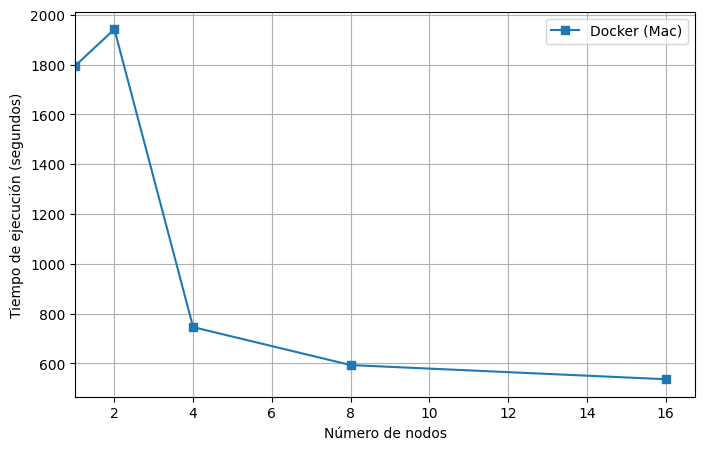
\includegraphics[width=0.8\textwidth]{imagenes/cap5/multi-node_mac_docker_time.png}
    \caption{Tiempo de ejecución en función del número de hebras en contenedores de MacOS(CPU) en entorno multiproceso.}
    \label{fig:multi-node_mac_docker_time}
\end{figure}

En la tabla \ref{tab:multi-node_mac_docker} se presentan los tiempos de ejecución y la reducción porcentual respecto a una hebra.

\begin{table}[ht]
    \centering
    \begin{tabular}{|c|c|c|}
        \hline
        \textbf{Procesos} & \textbf{Tiempo (s)} & \textbf{$\Delta$\% vs 1 proceso} \\
        \hline
        1.00              & 1794.98             & 0.00                             \\
        2.00              & 1942.42             & 8.21                             \\
        4.00              & 745.84              & -58.45                           \\
        8.00              & 593.47              & -66.94                           \\
        16.00             & 536.60              & -70.11                           \\
        \hline
    \end{tabular}
    \caption{Tiempos de ejecución y reducción porcentual respecto a un proceso en entorno multiproceso con contenedores de MacOS (CPU).}
    \label{tab:multi-node_mac_docker}
\end{table}

La tabla muestra la evolución del tiempo de ejecución al aumentar el número de procesos en un entorno multiproceso con contenedores de \textit{Docker} sobre MacOS utilizando CPU. Con un solo proceso, se establece el tiempo de referencia. Al pasar a dos procesos, se observa un incremento del 8.21\% en el tiempo de ejecución, lo que indica que la paralelización inicial introduce una penalización, probablemente debida a la sobrecarga de coordinación o a limitaciones en la gestión de recursos en el entorno de contenedores sobre MacOS. Sin embargo, al aumentar a cuatro procesos, el tiempo de ejecución disminuye de manera significativa, con una reducción del 58.45\%, lo que evidencia una mejora notable en el rendimiento gracias a la paralelización. Esta tendencia positiva se mantiene al escalar a ocho y dieciséis procesos, donde las reducciones alcanzan el 66.94\% y el 70.11\% respectivamente, mostrando que el sistema es capaz de aprovechar de manera eficiente los recursos adicionales a medida que se incrementa el número de procesos. En conjunto, los resultados indican que, aunque existe una penalización inicial al duplicar los procesos, el entorno multiproceso con contenedores de \textit{Docker} en MacOS logra una escalabilidad efectiva y una mejora sustancial del rendimiento a partir de cuatro procesos, confirmando la viabilidad de esta tecnología para la ejecución de aplicaciones paralelas en este contexto.

En la figura \ref{fig:multi-node_mac_podman_time} se muestra el tiempo de ejecución para la configuración de CPU en un entorno multiproceso con contenedores de \textit{Podman} en MacOS.

\begin{figure}[ht]
    \centering
    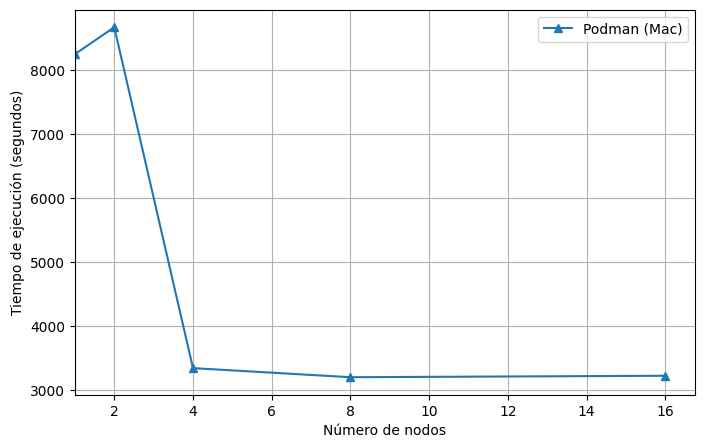
\includegraphics[width=0.8\textwidth]{imagenes/cap5/multi-node_mac_podman_time.png}
    \caption{Tiempo de ejecución en función del número de hebras en contenedores de \textit{Podman} (CPU) en entorno multiproceso.}
    \label{fig:multi-node_mac_podman_time}
\end{figure}

En la tabla \ref{tab:multi-node_mac_podman} se presentan los tiempos de ejecución y la reducción porcentual respecto a una hebra.

\begin{table}[ht]
    \centering
    \begin{tabular}{|c|c|c|}
        \hline
        \textbf{Procesos} & \textbf{Tiempo (s)} & \textbf{$\Delta$\% vs 1 proceso} \\
        \hline
        1.00              & 8247.00             & 0.00                             \\
        2.00              & 8668.00             & 5.10                             \\
        4.00              & 3343.15             & -59.46                           \\
        8.00              & 3201.07             & -61.19                           \\
        16.00             & 3223.98             & -60.91                           \\
        \hline
    \end{tabular}
    \caption{Tiempos de ejecución y reducción porcentual respecto a un proceso en entorno multiproceso con contenedores de \textit{Podman} en MacOS (CPU).}
    \label{tab:multi-node_mac_podman}
\end{table}

La tabla muestra la evolución del tiempo de ejecución al aumentar el número de procesos en un entorno multiproceso con contenedores de \textit{Podman} sobre MacOS utilizando CPU. Con un solo proceso, el tiempo de ejecución es el más alto y sirve como referencia. Al pasar a dos procesos, se observa un incremento del 5.10\% en el tiempo de ejecución, lo que indica que la paralelización inicial introduce una penalización, probablemente relacionada con la sobrecarga de coordinación o limitaciones en la gestión de recursos en este entorno. Sin embargo, al aumentar a cuatro procesos, el tiempo de ejecución disminuye de manera muy significativa, con una reducción del 59.46\%, lo que refleja una mejora notable en el rendimiento gracias a la paralelización. Esta mejora se mantiene al escalar a ocho y dieciséis procesos, donde las reducciones se sitúan en torno al 61\%, mostrando que el sistema es capaz de aprovechar de manera eficiente los recursos adicionales a partir de cuatro procesos. En conjunto, los resultados indican que, aunque existe una penalización inicial al duplicar los procesos, el entorno multiproceso con contenedores de \textit{Podman} en MacOS logra una escalabilidad efectiva y una mejora sustancial del rendimiento a partir de cuatro procesos, confirmando la viabilidad de esta tecnología para la ejecución de aplicaciones paralelas en este contexto.

\section{Pruebas de barrido de hebras}
\subsection{Ejecución en Ubuntu en nativo}
\subsubsection{CPU}

En la figura \ref{fig:thread_sweep_ubuntu_cpu_native_time} se muestra el tiempo de ejecución para la configuración de CPU en un entorno nativo con Ubuntu.

\begin{figure}[ht]
    \centering
    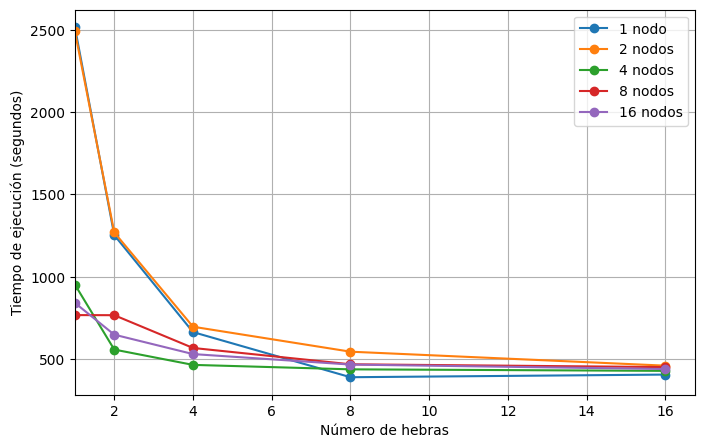
\includegraphics[width=0.8\textwidth]{imagenes/cap5/thread_sweep_ubuntu_cpu_native_time.png}
    \caption{Tiempo de ejecución en función del número de hebras en entorno nativo de Ubuntu (CPU).}
    \label{fig:thread_sweep_ubuntu_cpu_native_time}
\end{figure}

En la tabla \ref{tab:thread_sweep_ubuntu_cpu_native} se presentan los tiempos de ejecución y la reducción porcentual respecto a una hebra.

\begin{table}[ht]
    \centering
    \begin{tabular}{|c|c|c|c|}
        \hline
        \textbf{Procesos} & \textbf{Hebras} & \textbf{Tiempo (s)} & \textbf{$\Delta$\% vs 1 hebra} \\
        \hline
        1.00              & 1.00            & 2515.21             & 0.00                           \\
        1.00              & 2.00            & 1253.18             & -50.18                         \\
        1.00              & 4.00            & 664.69              & -73.57                         \\
        1.00              & 8.00            & 390.72              & -84.47                         \\
        1.00              & 16.00           & 406.76              & -83.83                         \\
        2.00              & 1.00            & 2489.49             & 0.00                           \\
        2.00              & 2.00            & 1269.36             & -49.01                         \\
        2.00              & 4.00            & 697.22              & -71.99                         \\
        2.00              & 8.00            & 545.73              & -78.08                         \\
        2.00              & 16.00           & 460.89              & -81.49                         \\
        4.00              & 1.00            & 952.85              & 0.00                           \\
        4.00              & 2.00            & 558.59              & -41.38                         \\
        4.00              & 4.00            & 465.64              & -51.13                         \\
        4.00              & 8.00            & 438.55              & -53.97                         \\
        4.00              & 16.00           & 429.30              & -54.95                         \\
        8.00              & 1.00            & 767.87              & 0.00                           \\
        8.00              & 2.00            & 767.21              & -0.09                          \\
        8.00              & 4.00            & 568.34              & -25.98                         \\
        8.00              & 8.00            & 469.23              & -38.89                         \\
        8.00              & 16.00           & 452.19              & -41.11                         \\
        16.00             & 1.00            & 841.96              & 0.00                           \\
        16.00             & 2.00            & 649.02              & -22.92                         \\
        16.00             & 4.00            & 531.22              & -36.91                         \\
        16.00             & 8.00            & 467.56              & -44.47                         \\
        16.00             & 16.00           & 440.44              & -47.69                         \\
        \hline
    \end{tabular}
    \caption{Tiempos de ejecución y reducción porcentual respecto a una hebra para distintas combinaciones de procesos y hebras en entorno nativo de Ubuntu (CPU).}
    \label{tab:thread_sweep_ubuntu_cpu_native}
\end{table}

La tabla recoge los tiempos de ejecución y la reducción porcentual respecto a una hebra para distintas combinaciones de procesos y hebras en un entorno nativo de Ubuntu utilizando CPU. Al analizar los resultados, se observa que el mayor beneficio en la reducción del tiempo de ejecución se obtiene al incrementar el número de hebras en configuraciones de un solo proceso, alcanzando una reducción del 84.47\% con ocho hebras respecto a la ejecución secuencial. Sin embargo, al aumentar a dieciséis hebras, el tiempo de ejecución apenas mejora e incluso empeora ligeramente, lo que sugiere que el paralelismo óptimo se alcanza en torno a ocho hebras, probablemente coincidiendo con el número de núcleos físicos disponibles. Cuando se incrementa el número de procesos, la reducción porcentual respecto a una hebra disminuye progresivamente, y el beneficio de añadir más hebras es cada vez menor. Por ejemplo, con dieciséis procesos y dieciséis hebras, la reducción es del 47.69\%, muy inferior a la obtenida en el caso monoproceso. Esto indica que la sobrecarga de coordinación y comunicación entre procesos limita la eficiencia del paralelismo a medida que se incrementa el número de procesos, haciendo que el escalado no sea lineal. En resumen, el entorno nativo de Ubuntu permite un aprovechamiento muy eficiente del paralelismo en configuraciones monoproceso, pero la eficiencia disminuye al aumentar el número de procesos, especialmente cuando se superan los límites físicos de la arquitectura o se incrementa la complejidad de la comunicación entre procesos.

En la figura \ref{fig:thread_sweep_ubuntu_cpu_native_cpu} se muestra el uso de CPU para la configuración de CPU en un entorno nativo con Ubuntu.

\begin{figure}[ht]
    \centering
    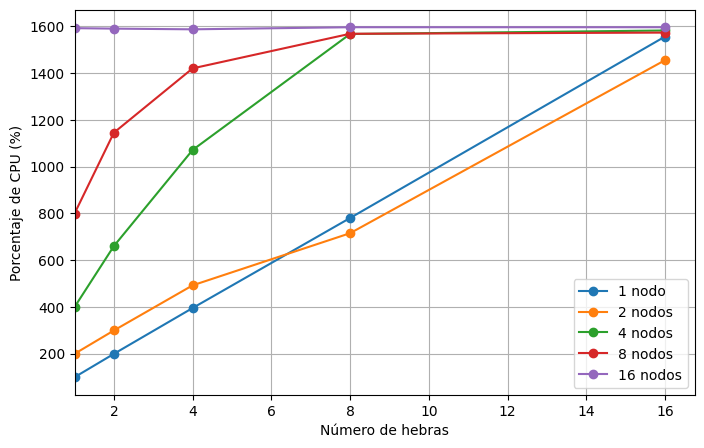
\includegraphics[width=0.8\textwidth]{imagenes/cap5/thread_sweep_ubuntu_cpu_native_cpu.png}
    \caption{Uso de CPU en función del número de hebras en entorno nativo de Ubuntu (CPU).}
    \label{fig:thread_sweep_ubuntu_cpu_native_cpu}
\end{figure}

En la tabla \ref{tab:thread_sweep_ubuntu_cpu_native_cpu} se presentan los valores de uso de CPU para distintas combinaciones de procesos y hebras.

\begin{table}[ht]
    \centering
    \begin{tabular}{|c|c|c|c|c|}
        \hline
        \textbf{Procesos} & \textbf{Hebras} & \textbf{CPU (\%)} & \textbf{Max (\%)} & \textbf{Efic. (\%)} \\
        \hline
        1.00              & 1.00            & 99.00             & 100.00            & 99.00               \\
        1.00              & 2.00            & 199.00            & 200.00            & 99.50               \\
        1.00              & 4.00            & 395.00            & 400.00            & 98.75               \\
        1.00              & 8.00            & 780.00            & 800.00            & 97.50               \\
        1.00              & 16.00           & 1556.00           & 1600.00           & 97.25               \\
        2.00              & 1.00            & 199.00            & 100.00            & 199.00              \\
        2.00              & 2.00            & 299.00            & 200.00            & 149.50              \\
        2.00              & 4.00            & 492.00            & 400.00            & 123.00              \\
        2.00              & 8.00            & 715.00            & 800.00            & 89.38               \\
        2.00              & 16.00           & 1455.00           & 1600.00           & 90.94               \\
        4.00              & 1.00            & 399.00            & 100.00            & 399.00              \\
        4.00              & 2.00            & 660.00            & 200.00            & 330.00              \\
        4.00              & 4.00            & 1071.00           & 400.00            & 267.75              \\
        4.00              & 8.00            & 1567.00           & 800.00            & 195.88              \\
        4.00              & 16.00           & 1582.00           & 1600.00           & 98.88               \\
        8.00              & 1.00            & 799.00            & 100.00            & 799.00              \\
        8.00              & 2.00            & 1145.00           & 200.00            & 572.50              \\
        8.00              & 4.00            & 1420.00           & 400.00            & 355.00              \\
        8.00              & 8.00            & 1568.00           & 800.00            & 196.00              \\
        8.00              & 16.00           & 1573.00           & 1600.00           & 98.31               \\
        16.00             & 1.00            & 1592.00           & 100.00            & 1592.00             \\
        16.00             & 2.00            & 1590.00           & 200.00            & 795.00              \\
        16.00             & 4.00            & 1587.00           & 400.00            & 396.75              \\
        16.00             & 8.00            & 1596.00           & 800.00            & 199.50              \\
        16.00             & 16.00           & 1596.00           & 1600.00           & 99.75               \\
        \hline
    \end{tabular}
    \caption{Valores de uso de CPU, máximo teórico y eficiencia para distintas combinaciones de procesos y hebras en entorno nativo de Ubuntu (CPU).}
    \label{tab:thread_sweep_ubuntu_cpu_native_cpu}
\end{table}

La tabla recoge el porcentaje de uso de CPU, el máximo teórico posible y la eficiencia alcanzada para diferentes combinaciones de procesos y hebras en un entorno nativo de Ubuntu. Cuando se utiliza un solo proceso, el uso de CPU crece de forma casi lineal con el número de hebras y la eficiencia se mantiene muy alta, siempre por encima del 97\%, lo que indica un excelente aprovechamiento de los recursos disponibles y una sobrecarga mínima asociada a la gestión de los hilos. Al aumentar el número de procesos, el uso total de CPU también crece, pero la eficiencia relativa disminuye de manera progresiva, especialmente cuando el número de hebras por proceso es bajo. Por ejemplo, con dos procesos y una hebra, la eficiencia es del 199\%, reflejando que se suman los recursos de ambos procesos, pero a medida que se incrementa el número de hebras, la eficiencia cae, situándose en torno al 90\% con dieciséis hebras. Este patrón se repite y se acentúa al escalar a cuatro, ocho y dieciséis procesos, donde la eficiencia solo se mantiene cercana al 100\% cuando el número de hebras por proceso es máximo. En configuraciones con muchos procesos y pocas hebras, la eficiencia es baja, lo que evidencia que la sobrecarga de coordinación y la distribución de tareas penalizan el aprovechamiento de los recursos. Sin embargo, cuando se asigna el máximo número de hebras por proceso, la eficiencia vuelve a valores cercanos al 100\%, lo que sugiere que el sistema es capaz de escalar eficazmente siempre que se maximice el paralelismo interno de cada proceso. En conjunto, estos resultados muestran que el entorno nativo de Ubuntu permite un uso muy eficiente de la CPU en configuraciones monoproceso y que, en escenarios multiproceso, la eficiencia depende en gran medida de la relación entre el número de procesos y el número de hebras asignadas a cada uno.

\subsubsection{CPU + GPU}

En la figura \ref{fig:thread_sweep_ubuntu_gpu_native_time} se muestra el tiempo de ejecución para la configuración de CPU + GPU en un entorno nativo con Ubuntu.

\begin{figure}[ht]
    \centering
    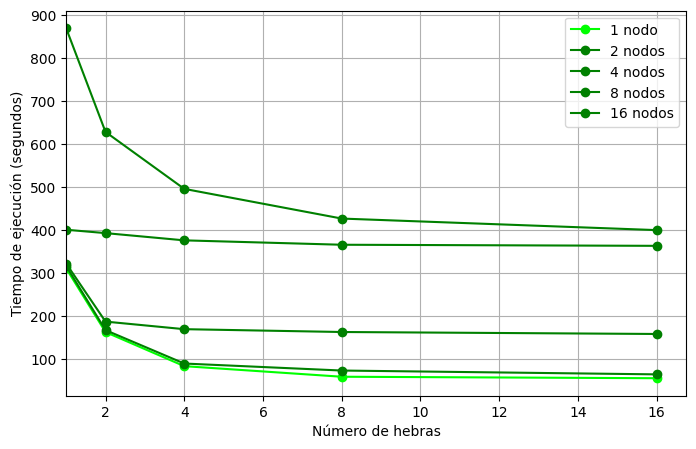
\includegraphics[width=0.8\textwidth]{imagenes/cap5/thread_sweep_ubuntu_gpu_native_time.png}
    \caption{Tiempo de ejecución en función del número de hebras en entorno nativo de Ubuntu (CPU + GPU).}
    \label{fig:thread_sweep_ubuntu_gpu_native_time}
\end{figure}

En la tabla \ref{tab:thread_sweep_ubuntu_gpu_native} se presentan los tiempos de ejecución y la reducción porcentual respecto a una hebra.

\begin{table}[ht]
    \centering
    \begin{tabular}{|c|c|c|c|}
        \hline
        \textbf{Procesos} & \textbf{Hebras} & \textbf{Tiempo (s)} & \textbf{$\Delta$\% vs 1 hebra} \\
        \hline
        1.00              & 1.00            & 311.68              & 0.00                           \\
        1.00              & 2.00            & 163.59              & -47.51                         \\
        1.00              & 4.00            & 84.49               & -72.89                         \\
        1.00              & 8.00            & 59.91               & -80.78                         \\
        1.00              & 16.00           & 56.45               & -81.89                         \\
        2.00              & 1.00            & 316.92              & 0.00                           \\
        2.00              & 2.00            & 168.14              & -46.95                         \\
        2.00              & 4.00            & 90.58               & -71.42                         \\
        2.00              & 8.00            & 74.30               & -76.56                         \\
        2.00              & 16.00           & 65.40               & -79.36                         \\
        4.00              & 1.00            & 322.77              & 0.00                           \\
        4.00              & 2.00            & 187.98              & -41.76                         \\
        4.00              & 4.00            & 170.38              & -47.21                         \\
        4.00              & 8.00            & 163.80              & -49.25                         \\
        4.00              & 16.00           & 159.22              & -50.67                         \\
        8.00              & 1.00            & 401.33              & 0.00                           \\
        8.00              & 2.00            & 393.50              & -1.95                          \\
        8.00              & 4.00            & 376.68              & -6.14                          \\
        8.00              & 8.00            & 366.47              & -8.69                          \\
        8.00              & 16.00           & 363.94              & -9.32                          \\
        16.00             & 1.00            & 869.40              & 0.00                           \\
        16.00             & 2.00            & 628.49              & -27.71                         \\
        16.00             & 4.00            & 496.28              & -42.92                         \\
        16.00             & 8.00            & 427.30              & -50.85                         \\
        16.00             & 16.00           & 400.48              & -53.94                         \\
        \hline
    \end{tabular}
    \caption{Tiempos de ejecución y reducción porcentual respecto a una hebra para distintas combinaciones de procesos y hebras en entorno nativo de Ubuntu (CPU + GPU).}
    \label{tab:thread_sweep_ubuntu_gpu_native}
\end{table}

La tabla recoge los tiempos de ejecución y la reducción porcentual respecto a una hebra para distintas combinaciones de procesos y hebras en un entorno nativo de Ubuntu utilizando CPU y GPU. Al analizar los resultados, se observa que el mayor beneficio en la reducción del tiempo de ejecución se obtiene al incrementar el número de hebras en configuraciones de un solo proceso, alcanzando una reducción del 81.89\% con dieciséis hebras respecto a la ejecución secuencial. El descenso del tiempo es especialmente acusado al pasar de una a dos hebras y de dos a cuatro, mientras que a partir de ocho hebras la mejora adicional es más limitada, lo que indica que el paralelismo óptimo se alcanza en torno a ese valor y que el sistema comienza a saturarse. Cuando se incrementa el número de procesos, la reducción porcentual respecto a una hebra disminuye progresivamente y el beneficio de añadir más hebras es cada vez menor. Por ejemplo, con dieciséis procesos y dieciséis hebras, la reducción es del 53.94\%, muy inferior a la obtenida en el caso monoproceso. Además, en configuraciones con ocho procesos o más, el incremento de hebras apenas aporta mejoras, lo que sugiere que la sobrecarga de coordinación y la gestión de la GPU entre procesos limita la eficiencia del paralelismo. En resumen, la combinación de CPU y GPU permite un aprovechamiento muy eficiente del paralelismo en configuraciones monoproceso, pero la eficiencia disminuye al aumentar el número de procesos, especialmente cuando se incrementa la complejidad de la comunicación y la gestión de recursos compartidos.

En la figura \ref{fig:thread_sweep_ubuntu_gpu_native_cpu} se muestra el uso de CPU para la configuración de CPU + GPU en un entorno nativo con Ubuntu.

\begin{figure}[ht]
    \centering
    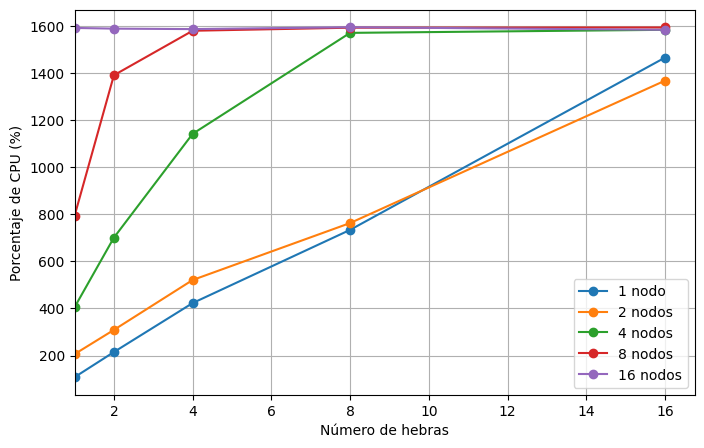
\includegraphics[width=0.8\textwidth]{imagenes/cap5/thread_sweep_ubuntu_gpu_native_cpu.png}
    \caption{Uso de CPU en función del número de hebras en entorno nativo de Ubuntu (CPU + GPU).}
    \label{fig:thread_sweep_ubuntu_gpu_native_cpu}
\end{figure}

En la tabla \ref{tab:thread_sweep_ubuntu_gpu_native_cpu} se presentan los valores de uso de CPU para distintas combinaciones de procesos y hebras.

\begin{table}[ht]
    \centering
    \begin{tabular}{|c|c|c|c|c|}
        \hline
        \textbf{Procesos} & \textbf{Hebras} & \textbf{CPU (\%)} & \textbf{Max (\%)} & \textbf{Efic. (\%)} \\
        \hline
        1.00              & 1.00            & 108.00            & 100.00            & 108.00              \\
        1.00              & 2.00            & 215.00            & 200.00            & 107.50              \\
        1.00              & 4.00            & 423.00            & 400.00            & 105.75              \\
        1.00              & 8.00            & 734.00            & 800.00            & 91.75               \\
        1.00              & 16.00           & 1466.00           & 1600.00           & 91.62               \\
        2.00              & 1.00            & 206.00            & 100.00            & 206.00              \\
        2.00              & 2.00            & 309.00            & 200.00            & 154.50              \\
        2.00              & 4.00            & 521.00            & 400.00            & 130.25              \\
        2.00              & 8.00            & 763.00            & 800.00            & 95.38               \\
        2.00              & 16.00           & 1368.00           & 1600.00           & 85.50               \\
        4.00              & 1.00            & 405.00            & 100.00            & 405.00              \\
        4.00              & 2.00            & 701.00            & 200.00            & 350.50              \\
        4.00              & 4.00            & 1142.00           & 400.00            & 285.50              \\
        4.00              & 8.00            & 1571.00           & 800.00            & 196.38              \\
        4.00              & 16.00           & 1584.00           & 1600.00           & 99.00               \\
        8.00              & 1.00            & 793.00            & 100.00            & 793.00              \\
        8.00              & 2.00            & 1391.00           & 200.00            & 695.50              \\
        8.00              & 4.00            & 1580.00           & 400.00            & 395.00              \\
        8.00              & 8.00            & 1593.00           & 800.00            & 199.12              \\
        8.00              & 16.00           & 1594.00           & 1600.00           & 99.62               \\
        16.00             & 1.00            & 1592.00           & 100.00            & 1592.00             \\
        16.00             & 2.00            & 1589.00           & 200.00            & 794.50              \\
        16.00             & 4.00            & 1587.00           & 400.00            & 396.75              \\
        16.00             & 8.00            & 1595.00           & 800.00            & 199.38              \\
        16.00             & 16.00           & 1584.00           & 1600.00           & 99.00               \\
        \hline
    \end{tabular}
    \caption{Valores de uso de CPU, uso máximo teórico y eficiencia para distintas combinaciones de procesos y hebras en entorno nativo de Ubuntu (CPU + GPU).}
    \label{tab:thread_sweep_ubuntu_gpu_native_cpu}
\end{table}

La tabla presenta los valores de uso de CPU, el máximo teórico y la eficiencia para diferentes combinaciones de procesos y hebras en un entorno nativo de Ubuntu utilizando CPU y GPU. En configuraciones monoproceso, el porcentaje de uso de CPU supera el 100\% en todos los casos, lo que refleja la contribución de la GPU al cómputo total y explica que la eficiencia calculada también supere el 100\% para valores bajos de hebras. A medida que se incrementa el número de hebras, la eficiencia disminuye ligeramente, situándose en torno al 91\% con 8 y 16 hebras, lo que indica que el sistema sigue aprovechando bien los recursos, aunque la saturación y la sobrecarga empiezan a notarse.

Al aumentar el número de procesos, el uso total de CPU crece de forma proporcional, pero la eficiencia relativa desciende de manera más acusada cuando el número de hebras por proceso es bajo, alcanzando valores muy elevados (por encima del 200\% o incluso del 700\% en algunos casos) debido a la suma de recursos de CPU y GPU en todos los procesos. Sin embargo, a medida que se incrementa el número de hebras, la eficiencia tiende a estabilizarse en torno al 99\% cuando se alcanza el máximo teórico de uso de CPU, lo que indica que el sistema es capaz de escalar eficazmente siempre que se maximice el paralelismo interno de cada proceso.

En conjunto, estos resultados muestran que la combinación de CPU y GPU permite un uso muy eficiente de los recursos en configuraciones monoproceso y que, en escenarios multiproceso, la eficiencia depende de la relación entre el número de procesos y el número de hebras asignadas, siendo óptima cuando se aprovechan al máximo las capacidades de cómputo de cada proceso.

% \subsubsection{Comparativa de rendimiento CPU vs CPU + GPU}

\subsection{Ejecución en contenedores de Ubuntu}
\subsubsection{CPU}

En la figura \ref{fig:thread_sweep_ubuntu_docker_time} se muestra el tiempo de ejecución para la configuración de CPU en un entorno con contenedores de Ubuntu.

\begin{figure}[ht]
    \centering
    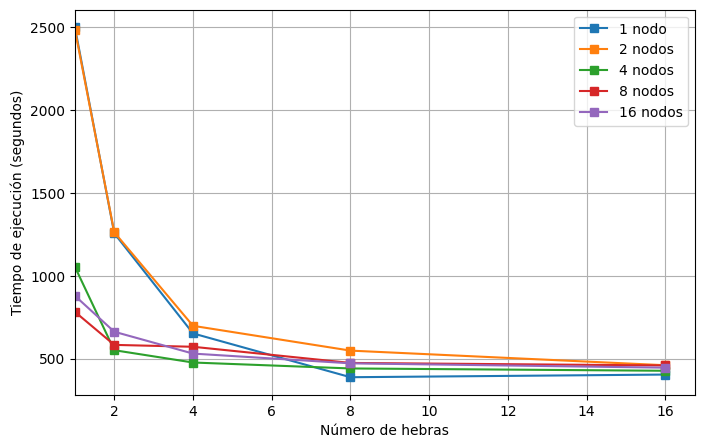
\includegraphics[width=0.8\textwidth]{imagenes/cap5/thread_sweep_ubuntu_docker_time.png}
    \caption{Tiempo de ejecución en función del número de hebras en contenedores de Ubuntu (CPU).}
    \label{fig:thread_sweep_ubuntu_docker_time}
\end{figure}

En la tabla \ref{tab:thread_sweep_ubuntu_docker_time} se presentan los tiempos de ejecución y la reducción porcentual respecto a una hebra.

\begin{table}[ht]
    \centering
    \begin{tabular}{|c|c|c|c|}
        \hline
        \textbf{Procesos} & \textbf{Hebras} & \textbf{Tiempo (s)} & \textbf{$\Delta$\% vs 1 hebra} \\
        \hline
        1.00              & 1.00            & 2499.09             & 0.00                           \\
        1.00              & 2.00            & 1255.95             & -49.74                         \\
        1.00              & 4.00            & 652.33              & -73.90                         \\
        1.00              & 8.00            & 388.04              & -84.47                         \\
        1.00              & 16.00           & 404.09              & -83.83                         \\
        2.00              & 1.00            & 2484.80             & 0.00                           \\
        2.00              & 2.00            & 1262.23             & -49.20                         \\
        2.00              & 4.00            & 698.05              & -71.91                         \\
        2.00              & 8.00            & 548.49              & -77.93                         \\
        2.00              & 16.00           & 460.29              & -81.48                         \\
        4.00              & 1.00            & 1054.20             & 0.00                           \\
        4.00              & 2.00            & 551.03              & -47.73                         \\
        4.00              & 4.00            & 476.76              & -54.78                         \\
        4.00              & 8.00            & 440.94              & -58.17                         \\
        4.00              & 16.00           & 426.96              & -59.50                         \\
        8.00              & 1.00            & 782.42              & 0.00                           \\
        8.00              & 2.00            & 583.08              & -25.48                         \\
        8.00              & 4.00            & 571.72              & -26.93                         \\
        8.00              & 8.00            & 474.19              & -39.39                         \\
        8.00              & 16.00           & 459.06              & -41.33                         \\
        16.00             & 1.00            & 879.20              & 0.00                           \\
        16.00             & 2.00            & 662.38              & -24.66                         \\
        16.00             & 4.00            & 530.59              & -39.65                         \\
        16.00             & 8.00            & 471.83              & -46.33                         \\
        16.00             & 16.00           & 445.63              & -49.31                         \\
        \hline
    \end{tabular}
    \caption{Tiempos de ejecución y reducción porcentual respecto a una hebra para distintas combinaciones de procesos y hebras en contenedores de Ubuntu (CPU).}
    \label{tab:thread_sweep_ubuntu_docker_time}
\end{table}

La tabla muestra los tiempos de ejecución y la reducción porcentual respecto a una hebra para distintas combinaciones de procesos y hebras en contenedores de Ubuntu utilizando CPU. Se observa que, en configuraciones monoproceso, el incremento del número de hebras produce una reducción muy significativa del tiempo de ejecución, alcanzando una disminución del 84.47\% con ocho hebras respecto a la ejecución secuencial. Sin embargo, al aumentar a dieciséis hebras, el tiempo de ejecución apenas mejora e incluso empeora ligeramente, lo que indica que el paralelismo óptimo se sitúa en torno a ocho hebras, probablemente coincidiendo con el número de núcleos físicos disponibles. Al incrementar el número de procesos, la reducción porcentual respecto a una hebra disminuye progresivamente y el beneficio de añadir más hebras es cada vez menor. Por ejemplo, con dieciséis procesos y dieciséis hebras, la reducción es del 49.31\%, notablemente inferior a la obtenida en el caso monoproceso. Además, en configuraciones con muchos procesos, el incremento de hebras aporta mejoras más limitadas, lo que sugiere que la sobrecarga de coordinación y la gestión de recursos entre contenedores penalizan la eficiencia del paralelismo. En conjunto, el entorno con contenedores de Ubuntu permite un aprovechamiento eficiente del paralelismo en configuraciones monoproceso, pero la eficiencia disminuye al aumentar el número de procesos, especialmente cuando se incrementa la complejidad de la comunicación y la gestión de procesos distribuidos.

En la figura \ref{fig:thread_sweep_ubuntu_podman_time} se muestra el tiempo de ejecución para la configuración de CPU en un entorno con contenedores de \textit{Podman}.

\begin{figure}[ht]
    \centering
    \includegraphics[width=0.8\textwidth]{imagenes/cap5/thread_sweep_ubuntu_podman_time.png}
    \caption{Tiempo de ejecución en función del número de hebras en contenedores de \textit{Podman} (CPU).}
    \label{fig:thread_sweep_ubuntu_podman_time}
\end{figure}

En la tabla \ref{tab:thread_sweep_ubuntu_podman_time} se presentan los tiempos de ejecución y la reducción porcentual respecto a una hebra.

\begin{table}[ht]
    \centering
    \begin{tabular}{|c|c|c|c|}
        \hline
        \textbf{Procesos} & \textbf{Hebras} & \textbf{Tiempo (s)} & \textbf{$\Delta$\% vs 1 hebra} \\
        \hline
        1.00              & 1.00            & 2499.16             & 0.00                           \\
        1.00              & 2.00            & 1266.51             & -49.32                         \\
        1.00              & 4.00            & 665.38              & -73.38                         \\
        1.00              & 8.00            & 400.51              & -83.97                         \\
        1.00              & 16.00           & 413.53              & -83.45                         \\
        2.00              & 1.00            & 2574.04             & 0.00                           \\
        2.00              & 2.00            & 1301.72             & -49.43                         \\
        2.00              & 4.00            & 724.50              & -71.85                         \\
        2.00              & 8.00            & 569.61              & -77.87                         \\
        2.00              & 16.00           & 467.63              & -81.83                         \\
        4.00              & 1.00            & 973.92              & 0.00                           \\
        4.00              & 2.00            & 567.28              & -41.75                         \\
        4.00              & 4.00            & 483.88              & -50.32                         \\
        4.00              & 8.00            & 448.66              & -53.93                         \\
        4.00              & 16.00           & 435.93              & -55.24                         \\
        8.00              & 1.00            & 796.84              & 0.00                           \\
        8.00              & 2.00            & 776.89              & -2.50                          \\
        8.00              & 4.00            & 581.62              & -27.01                         \\
        8.00              & 8.00            & 477.89              & -40.03                         \\
        8.00              & 16.00           & 464.91              & -41.66                         \\
        16.00             & 1.00            & 870.28              & 0.00                           \\
        16.00             & 2.00            & 661.10              & -24.04                         \\
        16.00             & 4.00            & 546.24              & -37.23                         \\
        16.00             & 8.00            & 480.46              & -44.79                         \\
        16.00             & 16.00           & 456.25              & -47.57                         \\
        \hline
    \end{tabular}
    \caption{Tiempos de ejecución y reducción porcentual respecto a una hebra para distintas combinaciones de procesos y hebras en contenedores de \textit{Podman} (CPU).}
    \label{tab:thread_sweep_ubuntu_podman_time}
\end{table}

La tabla recoge los tiempos de ejecución y la reducción porcentual respecto a una hebra para distintas combinaciones de procesos y hebras en contenedores de \textit{Podman} utilizando CPU. En configuraciones monoproceso, el incremento del número de hebras produce una reducción muy significativa del tiempo de ejecución, alcanzando una disminución del 83.97\% con ocho hebras respecto a la ejecución secuencial. Sin embargo, al aumentar a dieciséis hebras, el tiempo de ejecución apenas mejora e incluso empeora ligeramente, lo que indica que el paralelismo óptimo se sitúa en torno a ocho hebras, probablemente coincidiendo con el número de núcleos físicos disponibles. Al incrementar el número de procesos, la reducción porcentual respecto a una hebra disminuye progresivamente y el beneficio de añadir más hebras es cada vez menor. Por ejemplo, con dieciséis procesos y dieciséis hebras, la reducción es del 47.57\%, notablemente inferior a la obtenida en el caso monoproceso. Además, en configuraciones con muchos procesos, el incremento de hebras aporta mejoras más limitadas, lo que sugiere que la sobrecarga de coordinación y la gestión de recursos entre contenedores penalizan la eficiencia del paralelismo. En conjunto, el entorno con contenedores de \textit{Podman} permite un aprovechamiento eficiente del paralelismo en configuraciones monoproceso, pero la eficiencia disminuye al aumentar el número de procesos, especialmente cuando se incrementa la complejidad de la comunicación y la gestión de procesos distribuidos.

\subsubsection{CPU + GPU}

En la figura \ref{fig:thread_sweep_ubuntu_docker_gpu_time} se muestra el tiempo de ejecución para la configuración de CPU + GPU en un entorno con contenedores de Ubuntu.

\begin{figure}[ht]
    \centering
    \includegraphics[width=0.8\textwidth]{imagenes/cap5/thread_sweep_ubuntu_docker_gpu_time.png}
    \caption{Tiempo de ejecución en función del número de hebras en contenedores de Ubuntu (CPU + GPU).}
    \label{fig:thread_sweep_ubuntu_docker_gpu_time}
\end{figure}

En la tabla \ref{tab:thread_sweep_ubuntu_docker_gpu_time} se presentan los tiempos de ejecución y la reducción porcentual respecto a una hebra.

\begin{table}[ht]
    \centering
    \begin{tabular}{|c|c|c|c|}
        \hline
        \textbf{Procesos} & \textbf{Hebras} & \textbf{Tiempo (s)} & \textbf{$\Delta$\% vs 1 hebra} \\
        \hline
        1.00              & 1.00            & 312.18              & 0.00                           \\
        1.00              & 2.00            & 161.10              & -48.40                         \\
        1.00              & 4.00            & 85.78               & -72.52                         \\
        1.00              & 8.00            & 60.65               & -80.57                         \\
        1.00              & 16.00           & 57.45               & -81.60                         \\
        2.00              & 1.00            & 322.77              & 0.00                           \\
        2.00              & 2.00            & 166.99              & -48.26                         \\
        2.00              & 4.00            & 93.85               & -70.92                         \\
        2.00              & 8.00            & 74.22               & -77.01                         \\
        2.00              & 16.00           & 64.60               & -79.99                         \\
        4.00              & 1.00            & 329.54              & 0.00                           \\
        4.00              & 2.00            & 190.95              & -42.06                         \\
        4.00              & 4.00            & 174.85              & -46.94                         \\
        4.00              & 8.00            & 165.36              & -49.82                         \\
        4.00              & 16.00           & 159.15              & -51.71                         \\
        8.00              & 1.00            & 388.78              & 0.00                           \\
        8.00              & 2.00            & 390.25              & 0.38                           \\
        8.00              & 4.00            & 371.88              & -4.35                          \\
        8.00              & 8.00            & 365.06              & -6.10                          \\
        8.00              & 16.00           & 364.13              & -6.34                          \\
        16.00             & 1.00            & 847.37              & 0.00                           \\
        16.00             & 2.00            & 624.14              & -26.34                         \\
        16.00             & 4.00            & 486.42              & -42.60                         \\
        16.00             & 8.00            & 425.37              & -49.80                         \\
        16.00             & 16.00           & 393.49              & -53.56                         \\
        \hline
    \end{tabular}
    \caption{Tiempos de ejecución y reducción porcentual respecto a una hebra para distintas combinaciones de procesos y hebras en contenedores \textit{Docker} de Ubuntu (CPU + GPU).}
    \label{tab:thread_sweep_ubuntu_docker_gpu_time}
\end{table}

La tabla recoge los tiempos de ejecución y la reducción porcentual respecto a una hebra para distintas combinaciones de procesos y hebras en contenedores de Ubuntu utilizando CPU y GPU. En configuraciones monoproceso, el incremento del número de hebras produce una reducción muy significativa del tiempo de ejecución, alcanzando una disminución del 81.60\% con dieciséis hebras respecto a la ejecución secuencial. El mayor beneficio se observa al pasar de una a dos hebras y de dos a cuatro, mientras que a partir de ocho hebras la mejora adicional es más limitada, lo que indica que el paralelismo óptimo se alcanza en torno a ese valor y que el sistema comienza a saturarse. Al aumentar el número de procesos, la reducción porcentual respecto a una hebra disminuye progresivamente y el beneficio de añadir más hebras es cada vez menor. Por ejemplo, con dieciséis procesos y dieciséis hebras, la reducción es del 53.56\%, notablemente inferior a la obtenida en el caso monoproceso. Además, en configuraciones con ocho procesos o más, el incremento de hebras apenas aporta mejoras, lo que sugiere que la sobrecarga de coordinación y la gestión de la GPU entre procesos limita la eficiencia del paralelismo. En conjunto, la combinación de CPU y GPU en contenedores de Ubuntu permite un aprovechamiento eficiente del paralelismo en configuraciones monoproceso, pero la eficiencia disminuye al aumentar el número de procesos, especialmente cuando se incrementa la complejidad de la comunicación y la gestión de recursos compartidos.

En la figura \ref{fig:thread_sweep_ubuntu_podman_gpu_time} se muestra el tiempo de ejecución para la configuración de CPU + GPU en un entorno con contenedores de \textit{Podman}.

\begin{figure}[ht]
    \centering
    \includegraphics[width=0.8\textwidth]{imagenes/cap5/thread_sweep_ubuntu_podman_gpu_time.png}
    \caption{Tiempo de ejecución en función del número de hebras en contenedores de \textit{Podman} (CPU + GPU).}
    \label{fig:thread_sweep_ubuntu_podman_gpu_time}
\end{figure}

En la tabla \ref{tab:thread_sweep_ubuntu_podman_gpu_time} se presentan los tiempos de ejecución y la reducción porcentual respecto a una hebra.

\begin{table}[ht]
    \centering
    \begin{tabular}{|c|c|c|c|}
        \hline
        \textbf{Procesos} & \textbf{Hebras} & \textbf{Tiempo (s)} & \textbf{$\Delta$\% vs 1 hebra} \\
        \hline
        1.00              & 1.00            & 314.51              & 0.00                           \\
        1.00              & 2.00            & 158.84              & -49.50                         \\
        1.00              & 4.00            & 85.62               & -72.78                         \\
        1.00              & 8.00            & 59.47               & -81.09                         \\
        1.00              & 16.00           & 57.12               & -81.84                         \\
        2.00              & 1.00            & 316.80              & 0.00                           \\
        2.00              & 2.00            & 164.58              & -48.05                         \\
        2.00              & 4.00            & 93.56               & -70.47                         \\
        2.00              & 8.00            & 74.18               & -76.58                         \\
        2.00              & 16.00           & 61.51               & -80.58                         \\
        4.00              & 1.00            & 326.20              & 0.00                           \\
        4.00              & 2.00            & 193.69              & -40.62                         \\
        4.00              & 4.00            & 171.80              & -47.33                         \\
        4.00              & 8.00            & 164.47              & -49.58                         \\
        4.00              & 16.00           & 162.10              & -50.31                         \\
        8.00              & 1.00            & 391.86              & 0.00                           \\
        8.00              & 2.00            & 387.68              & -1.07                          \\
        8.00              & 4.00            & 377.01              & -3.79                          \\
        8.00              & 8.00            & 366.63              & -6.44                          \\
        8.00              & 16.00           & 365.54              & -6.72                          \\
        16.00             & 1.00            & 850.18              & 0.00                           \\
        16.00             & 2.00            & 629.92              & -25.91                         \\
        16.00             & 4.00            & 496.97              & -41.55                         \\
        16.00             & 8.00            & 429.80              & -49.45                         \\
        16.00             & 16.00           & 398.66              & -53.11                         \\
        \hline
    \end{tabular}
    \caption{Tiempos de ejecución y reducción porcentual respecto a una hebra para distintas combinaciones de procesos y hebras en contenedores de \textit{Podman} (CPU + GPU).}
    \label{tab:thread_sweep_ubuntu_podman_gpu_time}
\end{table}

La tabla presenta los tiempos de ejecución y la reducción porcentual respecto a una hebra para distintas combinaciones de procesos y hebras en contenedores de \textit{Podman} utilizando CPU y GPU. En configuraciones monoproceso, el incremento del número de hebras produce una reducción muy significativa del tiempo de ejecución, alcanzando una disminución del 81.84\% con dieciséis hebras respecto a la ejecución secuencial. El mayor beneficio se observa al pasar de una a dos hebras y de dos a cuatro, mientras que a partir de ocho hebras la mejora adicional es más limitada, lo que indica que el paralelismo óptimo se alcanza en torno a ese valor y que el sistema comienza a saturarse. Al aumentar el número de procesos, la reducción porcentual respecto a una hebra disminuye progresivamente y el beneficio de añadir más hebras es cada vez menor. Por ejemplo, con dieciséis procesos y dieciséis hebras, la reducción es del 53.11\%, notablemente inferior a la obtenida en el caso monoproceso. Además, en configuraciones con ocho procesos o más, el incremento de hebras apenas aporta mejoras, lo que sugiere que la sobrecarga de coordinación y la gestión de la GPU entre procesos limita la eficiencia del paralelismo. En conjunto, la combinación de CPU y GPU en contenedores de \textit{Podman} permite un aprovechamiento eficiente del paralelismo en configuraciones monoproceso, pero la eficiencia disminuye al aumentar el número de procesos, especialmente cuando se incrementa la complejidad de la comunicación y la gestión de recursos compartidos.

\subsection{Ejecución en contenedores de Windows}
\subsubsection{CPU}

En la figura \ref{fig:thread_sweep_windows_docker_time} se muestra el tiempo de ejecución para la configuración de CPU en un entorno con contenedores de Windows.

\begin{figure}[ht]
    \centering
    \includegraphics[width=0.8\textwidth]{imagenes/cap5/thread_sweep_windows_docker_time.png}
    \caption{Tiempo de ejecución en función del número de hebras en contenedores \textit{Docker} de Windows (CPU).}
    \label{fig:thread_sweep_windows_docker_time}
\end{figure}

En la tabla \ref{tab:thread_sweep_windows_docker_time} se presentan los tiempos de ejecución y la reducción porcentual respecto a una hebra.

\begin{table}[ht]
    \centering
    \begin{tabular}{|c|c|c|c|}
        \hline
        \textbf{Procesos} & \textbf{Hebras} & \textbf{Tiempo (s)} & \textbf{$\Delta$\% vs 1 hebra} \\
        \hline
        1.00              & 1.00            & 3308.08             & 0.00                           \\
        1.00              & 2.00            & 1341.41             & -59.45                         \\
        1.00              & 4.00            & 816.06              & -75.33                         \\
        1.00              & 8.00            & 602.60              & -81.78                         \\
        1.00              & 16.00           & 453.44              & -86.29                         \\
        2.00              & 1.00            & 2708.91             & 0.00                           \\
        2.00              & 2.00            & 1497.01             & -44.74                         \\
        2.00              & 4.00            & 921.23              & -65.99                         \\
        2.00              & 8.00            & 650.28              & -75.99                         \\
        2.00              & 16.00           & 526.23              & -80.57                         \\
        4.00              & 1.00            & 1185.46             & 0.00                           \\
        4.00              & 2.00            & 757.13              & -36.13                         \\
        4.00              & 4.00            & 537.45              & -54.66                         \\
        4.00              & 8.00            & 488.12              & -58.82                         \\
        4.00              & 16.00           & 476.64              & -59.79                         \\
        8.00              & 1.00            & 1090.62             & 0.00                           \\
        8.00              & 2.00            & 731.08              & -32.97                         \\
        8.00              & 4.00            & 586.55              & -46.22                         \\
        8.00              & 8.00            & 512.87              & -52.97                         \\
        8.00              & 16.00           & 501.93              & -53.98                         \\
        16.00             & 1.00            & 930.79              & 0.00                           \\
        16.00             & 2.00            & 717.75              & -22.89                         \\
        16.00             & 4.00            & 586.84              & -36.95                         \\
        16.00             & 8.00            & 526.20              & -43.47                         \\
        16.00             & 16.00           & 497.09              & -46.60                         \\
        \hline
    \end{tabular}
    \caption{Tiempos de ejecución y reducción porcentual respecto a una hebra para distintas combinaciones de procesos y hebras en contenedores \textit{Docker} de Windows (CPU).}
    \label{tab:thread_sweep_windows_docker_time}
\end{table}

La tabla muestra los tiempos de ejecución y la reducción porcentual respecto a una hebra para distintas combinaciones de procesos y hebras en contenedores \textit{Docker} de Windows utilizando CPU. Se observa que, en configuraciones monoproceso, el incremento del número de hebras produce una reducción muy significativa del tiempo de ejecución, alcanzando una disminución del 86.29\% con dieciséis hebras respecto a la ejecución secuencial. El mayor beneficio se obtiene al pasar de una a dos hebras (-59.45\%) y de dos a cuatro hebras (-15.88\% adicional), lo que indica una excelente escalabilidad inicial. A medida que se incrementa el número de procesos, la reducción porcentual respecto a una hebra disminuye progresivamente y el beneficio de añadir más hebras es cada vez menor. Por ejemplo, con dieciséis procesos y dieciséis hebras, la reducción es del 46.60\%, notablemente inferior a la obtenida en el caso monoproceso. Además, en configuraciones con muchos procesos, el incremento de hebras sigue aportando mejoras, pero estas son más limitadas, lo que sugiere que la sobrecarga de coordinación y la gestión de recursos entre contenedores penalizan la eficiencia del paralelismo. En conjunto, \textit{Docker} sobre Windows permite un aprovechamiento eficiente del paralelismo en configuraciones monoproceso, pero la eficiencia disminuye al aumentar el número de procesos, especialmente cuando se incrementa la complejidad de la comunicación y la gestión de procesos distribuidos.

En la figura \ref{fig:thread_sweep_windows_podman_time} se muestra el tiempo de ejecución para la configuración de CPU en un entorno con contenedores de \textit{Podman}.

\begin{figure}[ht]
    \centering
    \includegraphics[width=0.8\textwidth]{imagenes/cap5/thread_sweep_windows_podman_time.png}
    \caption{Tiempo de ejecución en función del número de hebras en contenedores de \textit{Podman} (CPU).}
    \label{fig:thread_sweep_windows_podman_time}
\end{figure}

En la tabla \ref{tab:thread_sweep_windows_podman_time} se presentan los tiempos de ejecución y la reducción porcentual respecto a una hebra.

\begin{table}[ht]
    \centering
    \begin{tabular}{|c|c|c|c|}
        \hline
        \textbf{Procesos} & \textbf{Hebras} & \textbf{Tiempo (s)} & \textbf{$\Delta$\% vs 1 hebra} \\
        \hline
        1.00              & 1.00            & 2520.21             & 0.00                           \\
        1.00              & 2.00            & 1359.69             & -46.05                         \\
        1.00              & 4.00            & 815.04              & -67.66                         \\
        1.00              & 8.00            & 595.54              & -76.37                         \\
        1.00              & 16.00           & 448.43              & -82.21                         \\
        2.00              & 1.00            & 2675.94             & 0.00                           \\
        2.00              & 2.00            & 1506.57             & -43.70                         \\
        2.00              & 4.00            & 921.20              & -65.57                         \\
        2.00              & 8.00            & 662.40              & -75.25                         \\
        2.00              & 16.00           & 531.13              & -80.15                         \\
        4.00              & 1.00            & 1228.59             & 0.00                           \\
        4.00              & 2.00            & 754.03              & -38.63                         \\
        4.00              & 4.00            & 542.63              & -55.83                         \\
        4.00              & 8.00            & 489.36              & -60.17                         \\
        4.00              & 16.00           & 474.74              & -61.36                         \\
        8.00              & 1.00            & 1089.75             & 0.00                           \\
        8.00              & 2.00            & 731.20              & -32.90                         \\
        8.00              & 4.00            & 591.11              & -45.76                         \\
        8.00              & 8.00            & 512.87              & -52.94                         \\
        8.00              & 16.00           & 503.82              & -53.77                         \\
        16.00             & 1.00            & 933.45              & 0.00                           \\
        16.00             & 2.00            & 718.20              & -23.06                         \\
        16.00             & 4.00            & 591.53              & -36.63                         \\
        16.00             & 8.00            & 527.98              & -43.44                         \\
        16.00             & 16.00           & 496.62              & -46.80                         \\
        \hline
    \end{tabular}
    \caption{Tiempos de ejecución y reducción porcentual respecto a una hebra para distintas combinaciones de procesos y hebras en contenedores de \textit{Podman} sobre Windows (CPU).}
    \label{tab:thread_sweep_windows_podman_time}
\end{table}

La tabla muestra los tiempos de ejecución y la reducción porcentual respecto a una hebra para distintas combinaciones de procesos y hebras en contenedores de \textit{Podman} sobre Windows (CPU). Se observa que, en configuraciones monoproceso, el incremento del número de hebras produce una reducción significativa del tiempo de ejecución, alcanzando una disminución del 82.21\% con 16 hebras respecto a la ejecución secuencial. El mayor beneficio se obtiene al pasar de 1 a 2 hebras (-46.05\%) y de 2 a 4 hebras (-21.61\% adicional), lo que indica una buena escalabilidad inicial. A medida que se incrementa el número de procesos, la reducción porcentual respecto a una hebra disminuye progresivamente y el beneficio de añadir más hebras es cada vez menor. Por ejemplo, con 16 procesos y 16 hebras, la reducción es del 46.80\%, notablemente inferior a la obtenida en el caso monoproceso. Además, en configuraciones con muchos procesos, el incremento de hebras sigue aportando mejoras, pero estas son más limitadas, lo que sugiere que la sobrecarga de coordinación y la gestión de recursos entre contenedores penalizan la eficiencia del paralelismo. En conjunto, \textit{Podman} sobre Windows permite un aprovechamiento eficiente del paralelismo en configuraciones monoproceso, pero la eficiencia disminuye al aumentar el número de procesos, especialmente cuando se incrementa la complejidad de la comunicación y la gestión de procesos distribuidos.

\subsubsection{CPU + GPU}

\subsection{Ejecución en contenedores de MacOS}
\subsubsection{CPU}

En la figura \ref{fig:thread_sweep_mac_docker_time} se muestra el tiempo de ejecución para la configuración de CPU en un entorno con contenedores de MacOS.

\begin{figure}[ht]
    \centering
    \includegraphics[width=0.8\textwidth]{imagenes/cap5/thread_sweep_mac_docker_time.png}
    \caption{Tiempo de ejecución en función del número de hebras en contenedores \textit{Docker} de MacOS (CPU).}
    \label{fig:thread_sweep_mac_docker_time}
\end{figure}

En la tabla \ref{tab:thread_sweep_mac_docker_time} se presentan los tiempos de ejecución y la reducción porcentual respecto a una hebra.

\begin{table}[ht]
    \centering
    \begin{tabular}{|c|c|c|c|}
        \hline
        \textbf{Procesos} & \textbf{Hebras} & \textbf{Tiempo (s)} & \textbf{$\Delta$\% vs 1 hebra} \\
        \hline
        1.00              & 1.00            & 1794.98             & 0.00                           \\
        1.00              & 2.00            & 951.56              & -46.99                         \\
        1.00              & 4.00            & 551.41              & -69.28                         \\
        1.00              & 8.00            & 304.35              & -83.04                         \\
        1.00              & 16.00           & 270.25              & -84.94                         \\
        2.00              & 1.00            & 1942.42             & 0.00                           \\
        2.00              & 2.00            & 994.15              & -48.82                         \\
        2.00              & 4.00            & 534.05              & -72.51                         \\
        2.00              & 8.00            & 318.04              & -83.63                         \\
        2.00              & 16.00           & 288.41              & -85.15                         \\
        4.00              & 1.00            & 745.84              & 0.00                           \\
        4.00              & 2.00            & 429.82              & -42.37                         \\
        4.00              & 4.00            & 296.17              & -60.29                         \\
        4.00              & 8.00            & 275.30              & -63.09                         \\
        4.00              & 16.00           & 263.92              & -64.61                         \\
        8.00              & 1.00            & 593.47              & 0.00                           \\
        8.00              & 2.00            & 388.01              & -34.62                         \\
        8.00              & 4.00            & 326.75              & -44.94                         \\
        8.00              & 8.00            & 303.35              & -48.89                         \\
        8.00              & 16.00           & 280.15              & -52.79                         \\
        16.00             & 1.00            & 536.60              & 0.00                           \\
        16.00             & 2.00            & 413.59              & -22.92                         \\
        16.00             & 4.00            & 319.30              & -40.50                         \\
        16.00             & 8.00            & 289.00              & -46.14                         \\
        16.00             & 16.00           & 271.75              & -49.36                         \\
        \hline
    \end{tabular}
    \caption{Tiempos de ejecución y reducción porcentual respecto a una hebra para distintas combinaciones de procesos y hebras en contenedores \textit{Docker} de MacOS (CPU).}
    \label{tab:thread_sweep_mac_docker_time}
\end{table}

La tabla muestra los tiempos de ejecución y la reducción porcentual respecto a una hebra para distintas combinaciones de procesos y hebras en contenedores \textit{Docker} de MacOS (CPU). Se observa que, en configuraciones monoproceso, el incremento del número de hebras produce una reducción muy significativa del tiempo de ejecución, alcanzando una disminución del 84.94\% con 16 hebras respecto a la ejecución secuencial. El mayor beneficio se obtiene al pasar de 1 a 2 hebras (-46.99\%) y de 2 a 4 hebras (-22.29\% adicional), lo que indica una buena escalabilidad inicial. A partir de 8 hebras, la mejora se estabiliza y el beneficio adicional es menor, lo que sugiere que el paralelismo óptimo se sitúa en torno a 8 hebras.

Al aumentar el número de procesos, la reducción porcentual respecto a una hebra sigue una tendencia similar: con 2 y 4 procesos se mantienen reducciones superiores al 60\%, pero a partir de 8 y 16 procesos las mejoras adicionales son más limitadas. Además, en algunos casos, como al pasar de 1 a 2 procesos, se observa un ligero aumento en el tiempo de ejecución, probablemente debido a la sobrecarga de coordinación entre procesos en el entorno de \textit{Docker} sobre MacOS.

En resumen, \textit{Docker} sobre MacOS permite un aprovechamiento eficiente del paralelismo hasta cierto punto, siendo recomendable utilizar hasta 8 hebras por proceso para maximizar el rendimiento. Aumentar el número de procesos y hebras más allá de ese valor aporta mejoras cada vez menores, debido a la sobrecarga de coordinación y a las limitaciones propias del entorno.

En la figura \ref{fig:thread_sweep_mac_podman_time} se muestra el tiempo de ejecución para la configuración de CPU en un entorno con contenedores de \textit{Podman}.

\begin{figure}[ht]
    \centering
    \includegraphics[width=0.8\textwidth]{imagenes/cap5/thread_sweep_mac_podman_time.png}
    \caption{Tiempo de ejecución en función del número de hebras en contenedores de \textit{Podman} (CPU).}
    \label{fig:thread_sweep_mac_podman_time}
\end{figure}

En la tabla \ref{tab:thread_sweep_mac_podman_time} se presentan los tiempos de ejecución y la reducción porcentual respecto a una hebra.

\begin{table}[ht]
    \centering
    \begin{tabular}{|c|c|c|c|}
        \hline
        \textbf{Procesos} & \textbf{Hebras} & \textbf{Tiempo (s)} & \textbf{$\Delta$\% vs 1 hebra} \\
        \hline
        1.00              & 1.00            & 8247.00             & 0.00                           \\
        1.00              & 2.00            & 4328.00             & -47.52                         \\
        1.00              & 4.00            & 2250.20             & -72.71                         \\
        1.00              & 8.00            & 1638.79             & -80.13                         \\
        1.00              & 16.00           & 1625.19             & -80.29                         \\
        2.00              & 1.00            & 8668.00             & 0.00                           \\
        2.00              & 2.00            & 4389.00             & -49.37                         \\
        2.00              & 4.00            & 2556.33             & -70.51                         \\
        2.00              & 8.00            & 1883.55             & -78.27                         \\
        2.00              & 16.00           & 1745.53             & -79.86                         \\
        4.00              & 1.00            & 3343.15             & 0.00                           \\
        4.00              & 2.00            & 2211.26             & -33.86                         \\
        4.00              & 4.00            & 1844.13             & -44.84                         \\
        4.00              & 8.00            & 1722.73             & -48.47                         \\
        4.00              & 16.00           & 1655.26             & -50.49                         \\
        8.00              & 1.00            & 3201.07             & 0.00                           \\
        8.00              & 2.00            & 2423.60             & -24.29                         \\
        8.00              & 4.00            & 2123.61             & -33.66                         \\
        8.00              & 8.00            & 1839.23             & -42.54                         \\
        8.00              & 16.00           & 1727.69             & -46.03                         \\
        16.00             & 1.00            & 3223.98             & 0.00                           \\
        16.00             & 2.00            & 2427.40             & -24.71                         \\
        16.00             & 4.00            & 2024.70             & -37.20                         \\
        16.00             & 8.00            & 1850.36             & -42.61                         \\
        16.00             & 16.00           & 1674.10             & -48.07                         \\
        \hline
    \end{tabular}
    \caption{Tiempos de ejecución y reducción porcentual respecto a una hebra para distintas combinaciones de procesos y hebras en contenedores de \textit{Podman} sobre MacOS (CPU).}
    \label{tab:thread_sweep_mac_podman_time}
\end{table}

La tabla muestra los tiempos de ejecución y la reducción porcentual respecto a una hebra para distintas combinaciones de procesos y hebras en contenedores de \textit{Podman} sobre MacOS (CPU). Se observa que, en configuraciones monoproceso, el incremento del número de hebras produce una reducción significativa del tiempo de ejecución, alcanzando una disminución del 80.29\% con 16 hebras respecto a la ejecución secuencial. El mayor beneficio se obtiene al pasar de 1 a 2 hebras (-47.52\%) y de 2 a 4 hebras (-25.19\% adicional), lo que indica una buena escalabilidad inicial. Sin embargo, a partir de 8 hebras, la mejora se estabiliza y el beneficio adicional es mínimo, sugiriendo que el paralelismo óptimo se sitúa en torno a 8 hebras.

Al aumentar el número de procesos, la reducción porcentual respecto a una hebra disminuye progresivamente. Por ejemplo, con 16 procesos y 16 hebras, la reducción es del 48.07\%, notablemente inferior a la obtenida en el caso monoproceso. Además, en configuraciones con muchos procesos, el incremento de hebras aporta mejoras cada vez más limitadas, lo que sugiere que la sobrecarga de coordinación y la gestión de recursos entre contenedores penalizan la eficiencia del paralelismo.

En resumen, \textit{Podman} sobre MacOS permite un aprovechamiento eficiente del paralelismo en configuraciones monoproceso, pero la eficiencia disminuye al aumentar el número de procesos, especialmente cuando se incrementa la complejidad de la comunicación y la gestión de procesos distribuidos. El punto óptimo de eficiencia se alcanza alrededor de 8 hebras por proceso.
%
\chapter{Conclusiones y trabajo futuro}\label{cap:conclusiones}

% [En este capítulo se presentan las conclusiones obtenidas al llevar a cabo el presente trabajo]

\section{Conclusiones}

% [En esta sección se presentan las principales conclusiones del trabajo realizado.]

El presente trabajo ha llevado a cabo un exhaustivo estudio experimental sobre el rendimiento y la escalabilidad de una aplicación de computación paralela y distribuida en distintos entornos y configuraciones, abarcando tanto la ejecución nativa como en contenedores (Docker y Podman), y considerando diferentes sistemas operativos (Ubuntu, Windows, MacOS), arquitecturas (CPU y CPU+GPU), y modos de operación (monoproceso, multiproceso y barrido de hebras). A continuación se resumen las principales conclusiones extraídas del análisis de todos los resultados obtenidos.

Se ha logrado embeber la aplicación \textit{HPMoon} en contenedores Docker y Podman, creando imágenes optimizadas que incluyen todas las dependencias necesarias para su ejecución. Esto ha permitido garantizar la portabilidad y reproducibilidad de los experimentos, facilitando la ejecución en diferentes plataformas sin necesidad de configurar manualmente el entorno. La comparación entre Docker y Podman ha mostrado que ambos sistemas ofrecen un rendimiento similar, con diferencias mínimas en los tiempos de ejecución, lo que confirma que Podman es una alternativa viable a Docker para este tipo de aplicaciones.

Los resultados obtenidos en los experimentos permiten extraer varias conclusiones clave sobre el comportamiento de HPMoon en diferentes entornos y configuraciones. En primer lugar, se observa que el incremento del número de hebras reduce de forma notable el tiempo de ejecución, alcanzando en configuraciones monoproceso eficiencias superiores al 97\% hasta el límite de núcleos físicos disponibles. El punto óptimo de paralelismo suele situarse en torno a las 8 hebras, que coincide con la arquitectura hardware analizada; a partir de ahí, los beneficios adicionales son escasos e incluso pueden aparecer ligeras penalizaciones por sobrecarga.

En cuanto a la ejecución multiproceso, la escalabilidad es efectiva hasta un cierto umbral, generalmente 4 u 8 procesos. Más allá de ese punto, la coordinación y la comunicación entre procesos introducen una sobrecarga que limita los beneficios del paralelismo. De hecho, en algunos escenarios, añadir más procesos puede llegar a empeorar el rendimiento, algo especialmente evidente en configuraciones con GPU o en entornos contenerizados, donde la gestión de recursos compartidos añade complejidad adicional.

Al comparar la ejecución nativa con la realizada en contenedores (Docker y Podman), se aprecia que el uso de contenedores no introduce penalizaciones relevantes: las diferencias suelen ser inferiores al 5\% y, en algunos casos, incluso se obtienen mejoras. Esto confirma la viabilidad de los contenedores como alternativa eficiente para ejecutar aplicaciones paralelas y distribuidas, manteniendo prácticamente el mismo nivel de rendimiento que en ejecución nativa.

En cuanto a los sistemas operativos, el dispositivo en el que se han realizado los experimentos de Ubuntu y Windows es el mismo, lo que permite una comparación directa. En este caso, Ubuntu ofrece de forma consistente los mejores resultados, con diferencias que pueden llegar a ser significativas en configuraciones multiproceso. Ubuntu es conocido por su eficiencia en la gestión de recursos y su optimización para cargas de trabajo intensivas, lo que se refleja en los tiempos de ejecución observados. Windows, aunque también es capaz de aprovechar el paralelismo, muestra un rendimiento inferior en comparación, lo cual puede atribuirse a diferencias en la gestión de hilos y procesos, así como a la sobrecarga inherente del sistema operativo. En el caso de MacOS la comparación no es directa, ya que el hardware es diferente. En este caso se buscaba evaluar la portabilidad y el rendimiento en un entorno distinto, cosa que se ha logrado parcialmente, ya que la falta de soporte para GPU limita las capacidades de paralelismo y aceleración.

La incorporación de GPU se traduce en una aceleración muy notable en escenarios monoproceso o con un bajo número de procesos, con reducciones de tiempo de entre el 80\% y el 88\%. No obstante, su escalabilidad es limitada en entornos distribuidos: al aumentar los procesos, la coordinación y la gestión compartida de la GPU penalizan el rendimiento, llegando incluso a hacer contraproducente su uso en configuraciones de gran tamaño.

De forma general, el análisis de los experimentos permite recomendar como configuración óptima el uso de 8 subpoblaciones y 8 hebras por proceso, lo que asegura un buen equilibrio entre eficiencia y aprovechamiento de recursos sin incurrir en sobrecarga. En configuraciones multiproceso, el número de procesos debe aumentarse con precaución, ya que el beneficio adicional disminuye rápidamente y puede revertirse si se añaden demasiados.

Finalmente, la utilización de contenedores se confirma como una herramienta clave para garantizar la portabilidad y la reproducibilidad de los experimentos. Gracias a ellos, es posible obtener resultados consistentes en diferentes plataformas y simplificar la gestión y el despliegue de entornos complejos de computación paralela y distribuida. Los resultados obtenidos demuestran que la aplicación analizada es capaz de aprovechar eficazmente el paralelismo y la aceleración por GPU en entornos monoproceso, y que la ejecución en contenedores es una alternativa plenamente válida a la ejecución nativa. Sin embargo, la escalabilidad en entornos multiproceso está limitada por la sobrecarga de coordinación y la gestión de recursos, especialmente al utilizar GPU. Estas conclusiones proporcionan una base sólida para la toma de decisiones en el diseño y despliegue de aplicaciones científicas y de ingeniería en entornos heterogéneos

\section{Retos y trabajo futuro}

A partir de los resultados obtenidos y del análisis detallado de los experimentos, se han identificado varios retos abiertos y posibles líneas de trabajo que pueden contribuir a mejorar tanto el rendimiento como la escalabilidad y la aplicabilidad de la solución propuesta.

Uno de los principales desafíos es la limitada escalabilidad observada al aumentar el número de procesos, especialmente en configuraciones con GPU. En este sentido, futuros estudios podrían centrarse en optimizar los mecanismos de comunicación y coordinación entre procesos, explorar alternativas de middleware más eficientes o incluso aplicar técnicas de balanceo dinámico de carga que reduzcan la sobrecarga y permitan aprovechar mejor los recursos distribuidos.

Otro aspecto clave es la gestión avanzada de recursos heterogéneos. La integración eficiente de CPU, GPU y otras posibles aceleradoras sigue siendo un reto, por lo que resulta interesante investigar estrategias inteligentes de asignación de tareas que se adapten dinámicamente a la disponibilidad y características de cada proceso, maximizando así el rendimiento global del sistema.

En lo referente a la automatización y portabilidad de los experimentos, aunque los contenedores ya han demostrado ser eficaces para garantizar reproducibilidad, aún queda margen de mejora. Incorporar herramientas de orquestación como Kubernetes o sistemas de gestión de flujos de trabajo científicos permitiría automatizar de manera más completa el ciclo experimental: desde el despliegue hasta la monitorización y la recolección de resultados.

Asimismo, el rápido avance de las arquitecturas hardware —con nuevas generaciones de GPU, aceleradores especializados y entornos de computación en la nube o en el edge— abre la puerta a extender este trabajo hacia escenarios emergentes, adaptando la infraestructura para sacar partido de sus capacidades. A ello se suma un aspecto cada vez más relevante: la eficiencia energética. Optimizar el consumo de recursos no solo permitiría reducir costes, sino también avanzar en sostenibilidad, identificando configuraciones que equilibren rendimiento y consumo energético.

Otra línea prometedora consiste en trasladar la metodología y las herramientas desarrolladas a otros problemas científicos o de ingeniería que también requieran computación paralela y distribuida. De esta forma, se ampliaría el alcance y el impacto del trabajo realizado. En paralelo, resulta fundamental validar la solución en clústeres reales de computación de alto rendimiento, lo que permitiría comprobar su robustez en entornos productivos y detectar cuellos de botella que no aparecen en escenarios locales.

Finalmente, se plantea como reto específico la posibilidad de explotar de forma combinada CPU y GPU en sistemas MacOS, especialmente en las nuevas arquitecturas Apple Silicon. Este avance permitiría superar las limitaciones actuales en dicho entorno, mejorando la portabilidad y aprovechando de forma más completa todos los recursos disponibles.

En resumen, aunque los resultados obtenidos confirman la viabilidad de la solución y aportan una base sólida, el camino hacia su mejora y ampliación es amplio. Los retos y líneas futuras aquí descritos ofrecen oportunidades tanto técnicas como aplicadas, que permitirán seguir avanzando en el desarrollo de soluciones más eficientes, portables y sostenibles en el ámbito de la computación paralela y distribuida.

%
\chapter{Bibliografía}\label{cap:conclusiones}



%
%
%%\nocite{*}
%\bibliography{bibliografia/bibliografia}\addcontentsline{toc}{chapter}{Bibliografía}
%\bibliographystyle{miunsrturl}
%
%\appendix
%\chapter{Anexo A}\label{cap:anexoA}

[En los anexos se expone aquella información que es complementaria a la propia memoria pero que, por su contenido o longitud, no encajan como un capítulo al uso. Piezas de código fuente, explicación en detalle de algoritmos, tablas adicionales, etc., son algunos ejemplos de información que podría ir en un anexo.]

%%\input{apendices/paper/paper}
%\input{glosario/entradas_glosario}
% \addcontentsline{toc}{chapter}{Glosario}
% \printglossary

\thispagestyle{empty}

\end{document}
